\documentclass[12pt,a4paper,oneside]{report}

% ============================================================
% config.tex
% Packages, layout, colors, custom commands, glossary, acronyms
% ============================================================

% ---------- Page geometry (ESPRIT guide: 2.5 cm margins) ----------
\usepackage[a4paper,margin=2.5cm]{geometry}

% ---------- Language ----------
\usepackage[french,english]{babel}
\selectlanguage{english}

% ---------- Fonts / encoding ----------
\usepackage[utf8]{inputenc}
\usepackage[T1]{fontenc}
\usepackage{lmodern}
\usepackage{times}          % Times New Roman-like body font (guide requirement)
\usepackage{microtype}
\setlength{\emergencystretch}{3em} % reduces overfull lines from long inline \texttt{} paths

% ---------- Line spacing / paragraphs (guide: 1.15, first-line indent 0.5 cm) ----------
\usepackage{setspace}
\setstretch{1.15}
\setlength{\parindent}{0.5cm}
% every paragraph starts with an indent, also the first one after a heading
\usepackage{indentfirst}

% ---------- Color ----------
\usepackage[table]{xcolor}
\definecolor{espritred}{RGB}{200,30,45}
\definecolor{espritdarkred}{RGB}{130,20,35}
\definecolor{espritgraydark}{RGB}{90,90,90}
\definecolor{espritgraylight}{RGB}{180,180,180}
\definecolor{codebg}{RGB}{245,245,245}
\definecolor{codekw}{RGB}{0,90,150}
\definecolor{codecomment}{RGB}{110,110,110}
\definecolor{codestring}{RGB}{150,30,30}

% ---------- Graphics / figures ----------
\usepackage{graphicx}
\graphicspath{{images/}{images/graphs/}{images/screenshots/}{images/logos/}{diagrams/}}
\usepackage{float}
\usepackage{subcaption}

% ---------- Page breaks ----------
% Figures and tables float ([htbp]) so that the text keeps filling a page instead of
% leaving an empty band when a figure does not fit; these limits let large figures
% share a page with text.
\renewcommand{\topfraction}{0.9}
\renewcommand{\bottomfraction}{0.8}
\renewcommand{\textfraction}{0.07}
\renewcommand{\floatpagefraction}{0.8}
\setcounter{topnumber}{3}
\setcounter{bottomnumber}{2}
\setcounter{totalnumber}{4}
% Pages that hold only figures or tables start at the top instead of being centred.
\makeatletter
\setlength{\@fptop}{0pt}
\setlength{\@fpsep}{\floatsep}
\setlength{\@fpbot}{0pt plus 1fil}
\makeatother
% A heading is never left at the bottom of a page with only a line or two under it:
% \Needspace{h} starts a new page when less than h of the page is left (same logic as
% the needspace package, defined here because that package is not installed).
\usepackage{etoolbox}
\makeatletter
\newcommand{\Needspace}[1]{\par\penalty-100\begingroup
  \setlength{\dimen@}{#1}%
  % On a page that has no text yet, the room left is \vsize, which LaTeX has already
  % reduced by the figures and tables placed at the top of that page.
  \ifdim\pagegoal=\maxdimen \dimen@ii\vsize \else \dimen@ii\pagegoal \fi
  \advance\dimen@ii-\pagetotal
  \ifdim\dimen@>\dimen@ii
    \ifdim\pagegoal=\maxdimen \ifdim\vsize<\textheight \null\fi\fi
    \ifdim\dimen@ii>\z@ \vfil\fi
    \break
  \fi\endgroup}
\makeatother
\pretocmd{\section}{\Needspace{13\baselineskip}}{}{\PackageWarning{config}{PATCHFAIL section}}
\pretocmd{\subsection}{\Needspace{7\baselineskip}}{}{\PackageWarning{config}{PATCHFAIL subsection}}
\pretocmd{\subsubsection}{\Needspace{6\baselineskip}}{}{\PackageWarning{config}{PATCHFAIL subsubsection}}
% Loaded after the heading check so that pending figures are placed first. A figure
% stays near its section: it may share a page with the start of the next one.
\usepackage[section,above,below]{placeins}
% When a section starts while figures of the previous one are still waiting, placeins
% ejects the page and, if they do not all fit at the top of the next one, uses \clearpage,
% which leaves a page with one figure and the new section alone on the page after. Here
% the waiting figures are placed page by page instead, and the text goes on under the
% last of them.
\makeatletter
\def\FloatBarrier{\par\begingroup\let\@elt\relax\@tempcnta\z@
  \loop
    \edef\@tempa{\@deferlist\@dbldeferlist}%
    \ifx\@tempa\@empty \@tempswafalse \else \@tempswatrue \fi
    \if@tempswa
      \ifdim\pagegoal=\maxdimen \ifx\@toplist\@empty \@tempcnta9 \fi\fi
      \ifnum\@tempcnta>6 \clearpage \@tempswafalse \fi
    \fi
  \if@tempswa
    \advance\@tempcnta\@ne
    \ifdim\pagegoal=\maxdimen \null\fi
    \newpage
  \repeat
  \endgroup\@fb@topbarrier}
\makeatother
\clubpenalty=10000
\widowpenalty=10000

% ---------- Tables ----------
\usepackage{amsmath}
\usepackage{booktabs}
\usepackage{longtable}
\usepackage{multirow}
\usepackage{array}
\usepackage{tabularx}
% prose columns of tables: ragged right, no stretched spaces
\newcolumntype{P}[1]{>{\raggedright\arraybackslash}p{#1}}
\newcolumntype{Y}{>{\raggedright\arraybackslash}X}
% long tables are not floats: they start right under the text that introduces them and
% continue on the next page with their header repeated
\usepackage{xltabular}
\setlength{\LTcapwidth}{\textwidth}
\setlength{\LTpre}{\medskipamount}
\setlength{\LTpost}{\medskipamount}

% ---------- Diagrams ----------
\usepackage{ifthen}
\usepackage{tikz}
\usetikzlibrary{arrows.meta,positioning,shapes.geometric,shapes.multipart,fit,backgrounds,calc,shadows}
\usepackage{pgfgantt}
\usepackage{pgfplots}
\pgfplotsset{compat=1.18}

% ---------- Code listings ----------
\usepackage{listings}
\lstdefinestyle{codestyle}{
    backgroundcolor=\color{codebg},
    commentstyle=\color{codecomment}\itshape,
    keywordstyle=\color{codekw}\bfseries,
    stringstyle=\color{codestring},
    basicstyle=\ttfamily\footnotesize,
    breakatwhitespace=false,
    breaklines=true,
    captionpos=b,
    keepspaces=true,
    numbers=left,
    numbersep=6pt,
    numberstyle=\tiny\color{gray},
    showspaces=false,
    showstringspaces=false,
    showtabs=false,
    tabsize=2,
    frame=single,
    framerule=0.3pt,
    rulecolor=\color{gray!40}
}
\lstset{style=codestyle}

% ---------- Hyperlinks / PDF bookmarks ----------
\usepackage{hyperref}
\hypersetup{
    colorlinks=true,
    linkcolor=blue,
    citecolor=blue,
    urlcolor=blue,
    filecolor=blue,
    bookmarksnumbered=true,
    bookmarksopen=true,
    plainpages=false,
    pdfpagelabels=true,
    pdftitle={CANvisionNative - PFE Report},
    pdfauthor={Mohamed Mootaz Ben Kraiem},
    pdfsubject={Final Year Engineering Project Report},
}
\usepackage[nameinlink,noabbrev]{cleveref} % must load after hyperref

% ---------- Acronyms / Glossary ----------
\usepackage[acronym,nomain,nonumberlist]{glossaries}
\makeglossaries
% ============================================================
% acronyms.tex — List of abbreviations used in the report
% ============================================================

\newacronym{can}{CAN}{Controller Area Network}
\newacronym{canfd}{CAN FD}{CAN with Flexible Data-rate}
\newacronym{uds}{UDS}{Unified Diagnostic Services}
\newacronym{isotp}{ISO-TP}{ISO Transport Protocol (ISO 15765-2)}
\newacronym{obd}{OBD-II}{On-Board Diagnostics, second generation}
\newacronym{bms}{BMS}{Battery Management System}
\newacronym{ids}{IDS}{Intrusion Detection System}
\newacronym{ml}{ML}{Machine Learning}
\newacronym{ai}{AI}{Artificial Intelligence}
\newacronym{llm}{LLM}{Large Language Model}
\newacronym{nvd}{NVD}{National Vulnerability Database}
\newacronym{rag}{RAG}{Retrieval-Augmented Generation}
\newacronym{iforest}{IF}{Isolation Forest}
\newacronym{kmeans}{K-Means}{K-Means Clustering}
\newacronym{svm}{SVM}{Support Vector Machine}
\newacronym{lof}{LOF}{Local Outlier Factor}
\newacronym{dbc}{DBC}{CAN Database}
\newacronym{ev}{EV}{Electric Vehicle}
\newacronym{mf4}{MF4}{ASAM Measurement Data Format version 4}
\newacronym{api}{API}{Application Programming Interface}
\newacronym{rest}{REST}{Representational State Transfer}
\newacronym{gui}{GUI}{Graphical User Interface}
\newacronym{wpf}{WPF}{Windows Presentation Foundation}
\newacronym{mvvm}{MVVM}{Model-View-ViewModel}
\newacronym{json}{JSON}{JavaScript Object Notation}
\newacronym{http}{HTTP}{Hypertext Transfer Protocol}
\newacronym{csv}{CSV}{Comma-Separated Values}
\newacronym{ecu}{ECU}{Electronic Control Unit}
\newacronym{dos}{DoS}{Denial of Service}
\newacronym{fp}{FP}{False Positive}
\newacronym{fn}{FN}{False Negative}
\newacronym{fps}{FPS}{Frames Per Second}
\newacronym{pfe}{PFE}{Projet de Fin d'Études (Final Year Engineering Project)}
\newacronym{sdk}{SDK}{Software Development Kit}
\newacronym{qa}{QA}{Quality Assurance}
\newacronym{rc}{RC}{Release Candidate}
\newacronym{up}{UP}{Unified Process}
\newacronym{ttup}{2TUP}{Two Track Unified Process}
\newacronym{uml}{UML}{Unified Modeling Language}
\newacronym{furps}{FURPS+}{Functionality, Usability, Reliability, Performance, Supportability, plus constraints}


% ---------- Bibliography (IEEE style) ----------
\usepackage[backend=biber,style=ieee,sorting=none]{biblatex}
\addbibresource{references.bib}
\setlength{\bibitemsep}{3pt}

% ---------- Headers / footers ----------
\usepackage{fancyhdr}
\setlength{\headheight}{14pt}
\pagestyle{fancy}
\fancyhf{}
\fancyhead[L]{\small\leftmark}
\fancyhead[R]{\small\thepage}
\renewcommand{\headrulewidth}{0.4pt}
% ESPRIT band of triangles along the bottom edge of the page. The cover, the dedication and
% the back cover use the empty style, so they are the only pages without it.
\newcommand{\espritband}{\begin{tikzpicture}[remember picture,overlay]
  \node[anchor=south west,inner sep=0pt] at (current page.south west)
    {
\includegraphics[width=\paperwidth,height=40pt]{esprit_band.pdf}};
\end{tikzpicture}}
\fancyfoot[C]{\espritband}
\fancypagestyle{plain}{\fancyhf{}\fancyfoot[C]{\espritband\raisebox{14pt}[0pt][0pt]{\thepage}}\renewcommand{\headrulewidth}{0pt}}

% ---------- Section title numbering depth ----------
\setcounter{secnumdepth}{3}
% Sections are numbered within their chapter without the chapter number (1, 1.1, 1.1.1),
% so that no heading has more than three levels of numbering. Figures and tables keep the
% chapter number (Figure 2.1).
\renewcommand{\thesection}{\arabic{section}}
% A reference to a section remembers its chapter: \Sref{label} prints "Section 3" inside the
% same chapter and "Section 3 of Chapter 4" from another chapter.
\makeatletter
\DeclareRobustCommand{\chmark}[1]{\gdef\lastrefch{#1}}
\gdef\lastrefch{}
\renewcommand*{\p@section}{\chmark{\thechapter}}
\renewcommand*{\p@subsection}{\chmark{\thechapter}}
\renewcommand*{\p@subsubsection}{\chmark{\thechapter}}
\newcommand*{\thischapterid}{\thechapter}
\newcommand*{\Sref}[1]{%
  \gdef\lastrefch{}\sbox\z@{\ref*{#1}}%
  Section~\ref{#1}%
  \begingroup\edef\@tempa{\lastrefch}\edef\@tempb{\thischapterid}%
  \ifx\@tempa\@empty\else\ifx\@tempa\@tempb\else\ of Chapter~\lastrefch\fi\fi\endgroup}
\makeatother
\setcounter{tocdepth}{3}

% ---------- Custom commands ----------
\newcommand{\todofill}[1]{\textbf{[TO FILL: #1]}}
\newcommand{\code}[1]{\texttt{#1}}
% a logo with its name under it; the optional argument sets the height of the logo
\newcommand{\techlogo}[3][1.1cm]{\begin{tabular}[b]{@{}c@{}}\rule[-0.55cm]{0pt}{1.1cm}\raisebox{-0.5\height}{\includegraphics[height=#1]{#2}}\\[2pt]\footnotesize #3\end{tabular}}


\begin{document}

% ============================================================
% FRONT MATTER
% ============================================================
\pagenumbering{gobble}

% ============================================================
% Cover page (front) — official ESPRIT PFE cover artwork
% (thesis/images/cover_front_bg.jpg, extracted from the filled
% official template), with the variable text (year, specialty,
% title, author, supervisors) overlaid at the positions used in
% that template, in the template's sans serif typeface, and the
% Capgemini Engineering logo (vector) centred in its placeholder box.
% ============================================================
\begin{titlepage}
\newgeometry{margin=0cm}
\thispagestyle{empty}

\begin{tikzpicture}[remember picture, overlay]
\begin{scope}[shift={(current page.north west)}, x=1cm, y=-1cm]

% ---- official background artwork (logo, banner, decoration, accreditation row) ----
\node[anchor=north west, inner sep=0pt] at (0,0) {
\includegraphics[width=21cm,height=29.7cm]{cover_front_bg.jpg}};

% ---- academic year ----
\node[anchor=north west, font=\fontfamily{phv}\fontsize{26}{28}\selectfont\bfseries, text=espritred] at (6.96,4.55) {2025 - 2026};

% ---- specialty value (label "SPECIALTY :" is already in the background) ----
\node[anchor=north west, font=\fontfamily{phv}\fontsize{15}{17}\selectfont\bfseries, text=black] at (10.46,11.5) {INFORMATION TECHNOLOGY};

% ---- project title ----
% centred on the axis of the template headings (GRADUATION PROJECT, banner, specialty): x = 12.4 cm
\node[anchor=north, font=\fontfamily{phv}\fontsize{18}{20}\selectfont\bfseries, text=black] at (12.4,12.95) {CANvisionNative};
\node[anchor=north, align=center, font=\fontfamily{phv}\fontsize{11}{13.5}\selectfont, text=black] at (12.4,13.9) {A diagnostic and validation platform for the CAN traffic\\of Battery Management Systems};

% ---- author / supervisors ----
\node[anchor=north west, font=\fontfamily{phv}\fontsize{12}{14}\selectfont, text=black] at (6.60,16.2) {\textbf{Prepared by:} Mohamed Mootaz Ben Kraiem};
\node[anchor=north west, font=\fontfamily{phv}\fontsize{12}{14}\selectfont, text=black] at (6.60,18.1) {\textbf{Academic Supervisor:} Mrs Nadia Boulifa};
\node[anchor=north west, font=\fontfamily{phv}\fontsize{12}{14}\selectfont, text=black] at (6.60,20.1) {\textbf{Corporate Supervisor:} Mr Hamda Guizani};

% ---- company logo, centred in the dotted placeholder box (x 9.83 to 17.01 cm, y 23.47 to 26.13 cm) ----
\node[anchor=center, inner sep=0pt] at (13.42,24.80) {
\includegraphics[width=6.0cm]{cover_capgemini_engineering.pdf}};

\end{scope}
\end{tikzpicture}

\end{titlepage}
\restoregeometry
\clearpage

% Validation form of ESPRIT (from "Page Garde Rapport Stage (Ang)"): it is inserted right after
% the cover page, then completed, signed and scanned.
\clearpage
\thispagestyle{empty}
\begingroup
\fontfamily{phv}\selectfont\small
\setstretch{1.6}
\vspace*{1cm}
\noindent Je valide le dépôt du rapport PFE relatif à l'étudiant nommé ci-dessous / I validate the submission of the student's report:

\begin{itemize}
    \item Nom \& Prénom / Name \& Surname : Mohamed Mootaz Ben Kraiem
\end{itemize}

\vspace{0.6cm}
\noindent\fbox{\begin{minipage}[t][6.2cm]{\dimexpr\textwidth-2\fboxsep-2\fboxrule\relax}
\vspace{0.3cm}
\centering{\normalsize Encadrant Entreprise / Business site Supervisor}\par
\vspace{0.5cm}
\raggedright
\begin{itemize}
    \item Nom \& Prénom / Name \& Surname : Hamda Guizani
\end{itemize}
\centering\footnotesize Cachet \& Signature / Stamp \& Signature
\end{minipage}}

\vspace{0.8cm}
\noindent\fbox{\begin{minipage}[t][6.2cm]{\dimexpr\textwidth-2\fboxsep-2\fboxrule\relax}
\vspace{0.3cm}
\centering{\normalsize Encadrant Académique / Academic Supervisor}\par
\vspace{0.5cm}
\raggedright
\begin{itemize}
    \item Nom \& Prénom / Name \& Surname : Nadia Boulifa
\end{itemize}
\centering Signature / Signature
\end{minipage}}

\vfill
\noindent{\footnotesize Ce formulaire doit être rempli, signé et \underline{scanné} / This form must be completed, signed and \underline{scanned}.\par
\noindent Ce formulaire doit être introduit après la page de garde / This form must be inserted after the cover page.\par}
\endgroup
\clearpage

% The dedication is a full page letter, made by dedication/make_letter.py
% (edit the words there and run it again).
\clearpage
\thispagestyle{empty}
\phantomsection
\addcontentsline{toc}{chapter}{Dedication}
\markboth{\MakeUppercase{Dedication}}{\MakeUppercase{Dedication}}
\begin{tikzpicture}[remember picture, overlay]
\node[anchor=north west, inner sep=0pt] at (current page.north west)
  {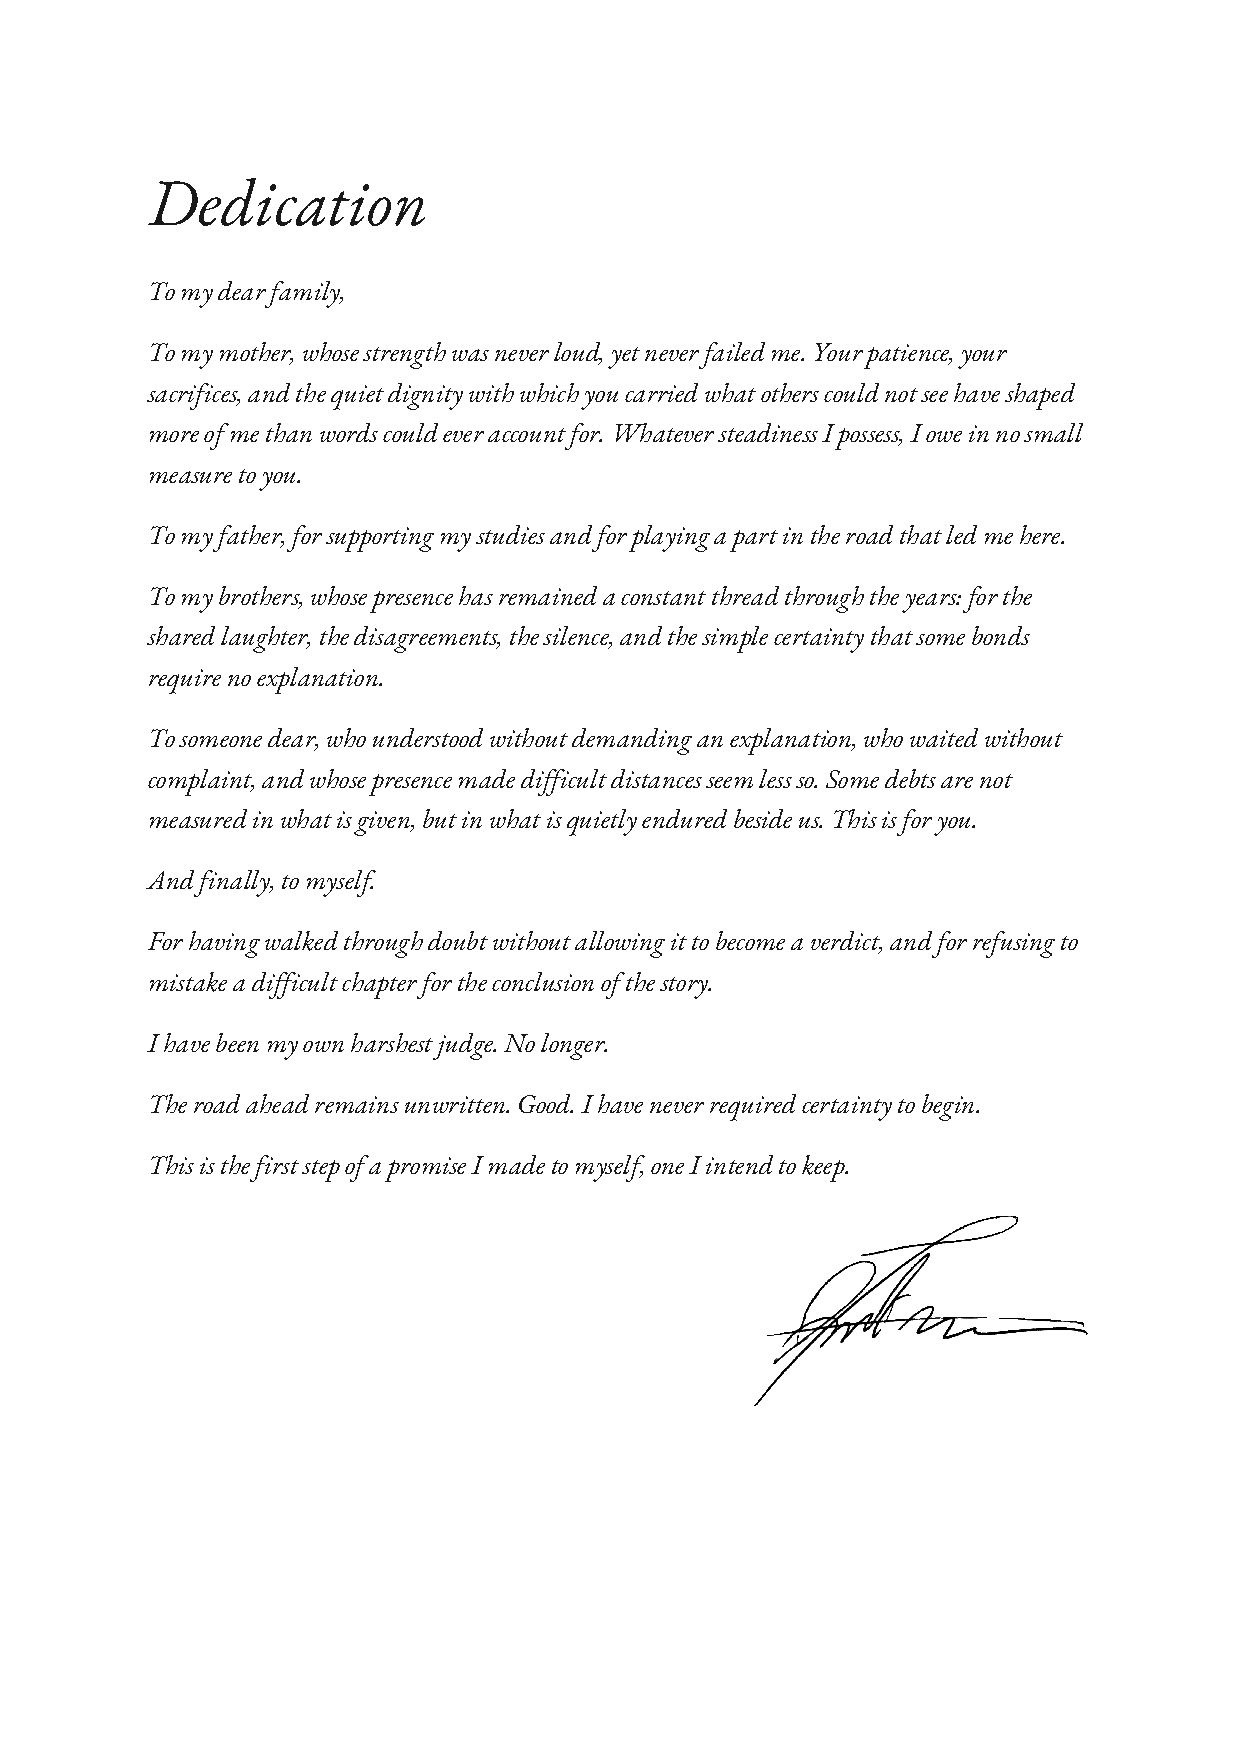
\includegraphics[width=\paperwidth,height=\paperheight]{dedication_letter.pdf}};
\end{tikzpicture}
\null
\clearpage

\chapter*{Acknowledgements}
\markboth{\MakeUppercase{Acknowledgements}}{\MakeUppercase{Acknowledgements}}
\addcontentsline{toc}{chapter}{Acknowledgements}

I would like to thank my academic supervisor at ESPRIT, Mrs Nadia Boulifa, for following this work from the beginning, for the time given to my questions, and for the advice that shaped this report.

I also thank my supervisor at Capgemini Engineering, Mr Hamda Guizani, for welcoming me into the Battery Management Systems team, for the trust placed in me during this work and study program, and for the guidance that helped me keep the project close to the real needs of the team. My thanks also go to the members of the Automotive division of Capgemini Tunisia for their availability and their help.

I thank my mother, for her love and for every sacrifice she made so that I could reach this point; my father, for supporting my studies; my brothers and my family, for their encouragement; and someone dear, for standing by my side every step of the way. To everyone who supported me, directly or indirectly, thank you.

Finally, I thank the members of the jury for agreeing to evaluate this work.

\cleardoublepage


\pagenumbering{roman}

% the lists are set with single line spacing so that the contents fit on three pages
\begingroup
\setstretch{1}
\tableofcontents
\clearpage
\listoffigures
\clearpage
\listoftables
\clearpage
\endgroup
\printglossary[type=\acronymtype,title={List of Abbreviations}]
% written out in the text, listed here as well
\glsadd{bms}\glsadd{svm}\glsadd{lof}
\clearpage

\chapter*{General Introduction}
\markboth{\MakeUppercase{General Introduction}}{\MakeUppercase{General Introduction}}
\addcontentsline{toc}{chapter}{General Introduction}

A modern vehicle is a small network of computers on wheels. An electric car contains many \glspl{ecu} that control braking, battery management, motor torque and driver assistance, and they exchange data mostly over the \gls{can} bus.

The \gls{can} protocol~\cite{iso11898} was designed in the 1980s for reliability. Every node can send and receive frames, and when two nodes talk at the same time, the message with the highest priority wins. This works very well on a closed network where every node can be trusted. It was never meant to resist someone who gains access to the bus: a frame carries no field for authentication and no encryption, so the bus cannot tell a genuine frame from a forged one.

Over the last fifteen years, security researchers have shown many times that this is not a theoretical problem. Experimental analyses of production vehicles~\cite{koscher2010experimental,checkoway2011comprehensive}, a remote attack on an unmodified car~\cite{miller2015remote} and public intrusion detection datasets~\cite{seo2018gids,verma2020road} have all shown that access to the \gls{can} bus can change the physical behaviour of a vehicle. At the same time, electric vehicles have added more safety critical messages to the bus, such as battery management and motor control, and more remote entry points, such as telematics, over the air updates and mobile applications.

Detecting anomalies on a \gls{can} bus is not the same problem as on a computer network: the frames carry at most 8 bytes, most are periodic, and their meaning changes from one vehicle to another. This calls for a system that looks at timing, payload and a learned model of normal behaviour, and that adapts to the vehicle it watches.

This report presents the design, the implementation and the validation of \textbf{CANvisionNative}, a diagnostic and validation platform for the \gls{can} traffic of Battery Management Systems. It gives a BMS engineer one view of the traffic, through replay, monitoring and anomaly detection, explains the anomalies in plain language and exports the results. A large part of the project went into validation: six defects were found and corrected on a real vehicle recording, and the rebuilt models were evaluated on recordings they had never seen.

This report follows the phases of the Unified Process. Chapter~\ref{chap:framework} presents the general framework of the project: the host company, the context, the existing solutions, the problem statement, the proposed solution, its objectives and the development methodology. Chapter~\ref{chap:inception} presents the inception phase: the actors, the functional and non functional requirements, the use case model, the initial risks and the plan. Chapter~\ref{chap:elaboration} presents the elaboration phase: the technical choices, the architecture, the analysis model, the dynamic view, the detection architecture, the framing of the machine learning problem and the architecture baseline. Chapter~\ref{chap:construction} presents the four iterations of the construction phase: the first detection pipeline and client, its validation and correction on a Kia EV6 recording, the hardware layer and its bench rig, and the rebuild of the models with their evaluation on recordings kept out of training. Chapter~\ref{chap:transition} presents the transition phase: the final release, its tests, the traceability of the requirements, the deployment and documentation, and the scope within which the software can be considered stable. The report ends with a general conclusion.

\cleardoublepage


% ============================================================
% MAIN MATTER
% ============================================================
\pagenumbering{arabic}
\setcounter{page}{1}

\chapter{General Framework}
\label{chap:framework}

\section*{Introduction}
\addcontentsline{toc}{section}{Introduction}

This chapter sets the frame of the project: the host company and team, the context of the work, the existing solutions, the problems the project addresses, the solution we propose, its objectives, and the development process we followed, the Unified Process.

\section{Host organization}

\subsection{Presentation}

This graduation project was carried out within a work and study program (alternance) at \textbf{Capgemini Engineering} (Figure~\ref{fig:capgemini-logo}), the engineering and research and development branch of the Capgemini group. The group, headquartered in France, provides consulting, digital transformation and engineering services to many industries. The automotive sector is one of them, where Capgemini works both on software systems and on embedded engineering.

\begin{figure}[H]
\centering

\includegraphics[width=0.45\textwidth]{cover_capgemini_engineering.pdf}
\caption{Logo of Capgemini Engineering.}
\label{fig:capgemini-logo}
\end{figure}

\subsection{Department and work context}

The program takes place in the Automotive division of Capgemini Tunisia, within the Battery Management Systems (BMS) team, which develops and validates the embedded software of battery management functions for electric and hybrid vehicles. Since September 2024, it has combined a full time position in this team, five days a week from 9 am to 6 pm, as a quality assurance (QA) tester of battery management software for BMW Group, with classes at ESPRIT on Saturdays. A large part of this work consists in checking the messages that the \glspl{ecu} exchange on the \gls{can} bus: whether a cell voltage, a temperature or a state of charge is sent at the expected rate and with a plausible value.

CANvisionNative is not one of the team's deliverables: it was built alongside this position, from February 2026. The idea came from the difficulties met in this daily validation work. Working inside a team that knows \gls{ecu} communication and automotive embedded software helped keep the project close to real needs.

\section{Project context}

An electric vehicle relies on its \gls{can} bus to let its \glspl{ecu} exchange data, and the Battery Management System is one of the busiest of them: it sends cell voltages, temperatures, currents and the state of charge many times per second. Validating a BMS therefore means reading a large amount of \gls{can} traffic and deciding, frame after frame, whether it behaves as expected.

The \gls{can} protocol was designed for reliability on a closed network. It gives no sender identity and no authentication, and the security literature has shown that it can be abused through message injection, flooding or replay~\cite{koscher2010experimental,lokman2019intrusion}. A validation toolchain that does not watch the bus cannot notice a malicious frame any more than a faulty one.

In this context, an engineer needs to work on recorded logs as well as on a live bus, to replay a session after a change, to see quickly which frames depart from the usual behaviour of the vehicle, and to understand why.

\section{Study of existing solutions}
\label{sec:existing}

The existing solutions fall into three categories. Figure~\ref{fig:existing-logos} shows the commercial and open source tools and the diagnostic standards discussed below.

\begin{figure}[H]
\centering
\begin{tabular}{ccccc}
\techlogo[0.62cm]{vector.pdf}{CANoe, CANalyzer} & \techlogo{savvycan.png}{SavvyCAN} & \techlogo{linux.pdf}{candump (can-utils)} & \techlogo[1cm]{sae.pdf}{SAE J1979 (\acrshort{obd})} & \techlogo[1cm]{iso.pdf}{ISO 14229 (\acrshort{uds})} \\
\end{tabular}
\caption[Existing tools and diagnostic standards.]{Existing tools and diagnostic standards: Vector CANoe and CANalyzer, SavvyCAN, candump from the Linux can-utils, and the SAE J1979 and ISO 14229 standards used by diagnostic scanners.}
\label{fig:existing-logos}
\end{figure}

\subsection{CAN analysers}

Commercial tools such as Vector CANoe~\cite{vector_canoe} and CANalyzer are the professional standard for observing \gls{can} traffic: they capture raw frames, decode them with a \gls{dbc} file and replay a recorded log. They show what is on the bus, but not whether a frame is normal for this vehicle, unless custom scripts are written on top of the product.

\subsection{Intrusion detection research}

Research on \gls{can} intrusion detection~\cite{lokman2019intrusion} follows three families. \textbf{Signature based detection} compares the traffic with known attack patterns and cannot recognise a new one. \textbf{Specification based detection} writes the expected behaviour by hand for every vehicle. \textbf{Anomaly based detection} learns normal traffic, for example from the timing of the messages~\cite{song2016intrusion,cho2016fingerprinting} or from its entropy~\cite{muter2011entropy}, and flags what deviates from it. These detectors usually rely on one signal, aim at attacks rather than at explaining the bus, and are evaluated on public benchmarks~\cite{seo2018gids,verma2020road}.

\subsection{Viewers and diagnostic scanners}

Open source utilities such as candump~\cite{canutils} and SavvyCAN~\cite{savvycan} display raw frames, with little control over replay and no notion of what is abnormal. Diagnostic scanners based on \gls{obd}, defined in SAE~J1979~\cite{sae_j1979}, or on \gls{uds}, defined in ISO~14229~\cite{iso14229}, ask specific \glspl{ecu} for known parameters, so they only see what they ask for.

\subsection{Synthesis}

Table~\ref{tab:existing-comparison} summarises these categories.

\begin{table}[H]
\centering
\small
\caption{Existing solutions and their limits for BMS validation work.}
\label{tab:existing-comparison}
\begin{tabularx}{\textwidth}{|P{2.9cm}|P{2.9cm}|Y|Y|}
\hline
\textbf{Solution or category} & \textbf{Main purpose} & \textbf{Strengths} & \textbf{Limitations relevant to this project} \\
\hline
\gls{can} analysers (Vector CANoe, CANalyzer) & Observe, decode and replay \gls{can} traffic & Professional standard; capture, \gls{dbc} decoding and replay through a rich, configurable interface & No judgement on whether a frame is normal for the vehicle without custom scripts \\
\hline
Intrusion detection research & Detect attacks on the \gls{can} bus & Signature based: precise on known attacks; specification based: needs no attack data; anomaly based: learns normal traffic, widely applicable & Usually one signal or one set of rules; aims at attacks rather than at explaining the bus; a model trained on one vehicle rarely transfers; no explanation of an alert \\
\hline
Open source viewers (candump, SavvyCAN) & Display and log raw frames & Lightweight and open source & Little control over replay; no notion of what is abnormal \\
\hline
Diagnostic scanners (\gls{obd}, \gls{uds}) & Request known parameters, such as fault codes, from specific \glspl{ecu} & Standard request and response protocols & Only see what they ask for; do not monitor the bus as a whole \\
\hline
\end{tabularx}
\end{table}

Three limits come back. A detector built on a single signal misses a problem that does not disturb that signal. A model trained on one vehicle rarely transfers to another, because message layouts, sending rates and value ranges differ, and choosing the right model is often treated as a detail. And no tool turns an anomaly score into an explanation an engineer can act on within one workflow.

\section{Problem statement}

Four problems of day to day BMS validation work motivated the project:

\begin{enumerate}
    \item \textbf{No live view of the traffic:} Reading raw frames says what happened, not whether it should have happened. By the time something odd is noticed in a spreadsheet or a log viewer, the context that would explain it is often lost.
    \item \textbf{Weak replay:} Replaying a session is central to validation, but the usual tools either replay frames without judging them or accept only a few log formats, so engineers convert files by hand or change tools in the middle of an investigation.
    \item \textbf{Scattered tools:} No single tool available to the team combines decoding, replay, live capture and anomaly detection. An engineer combines a \gls{can} analyser, a diagnostic scanner, and a spreadsheet for comparisons across sessions.
    \item \textbf{Alerts without explanation:} When a tool flags something, it is usually a bare number that does not say which pattern caused it or what to check next.
\end{enumerate}

The lack of security of the \gls{can} protocol (ISO~11898~\cite{iso11898}) makes these problems worse. Security is therefore a real but secondary motivation: the first goal is one clear and explainable view of the bus. The question this project answers is therefore: how can we give a BMS engineer one view of the \gls{can} traffic, adapted to each vehicle, that explains its own alerts, and show that it works on real recordings?

\section{Proposed solution}
\label{sec:proposed-solution}

We propose \textbf{CANvisionNative}, a diagnostic and validation platform for the \gls{can} traffic of Battery Management Systems. Diagnostics is its main purpose; live monitoring, log replay and anomaly detection are the means to serve it. It is made of four parts:

\begin{itemize}
    \item A Windows desktop client (\gls{wpf}, \gls{mvvm}) where the analyst imports a log, replays it and reviews the results.
    \item A Python backend (FastAPI) that reads recordings in several formats, decodes the frames when a \gls{dbc} file exists, scores each frame and explains the flagged ones in plain language.
    \item Machine learning models trained separately for each vehicle.
    \item Three traffic sources: recorded logs, a live simulator, and live capture from a \gls{can} adapter.
\end{itemize}

CANvisionNative does not compete with detection research; it gathers in one diagnostic workflow what the tools of \Sref{sec:existing} offer separately: replay of several log formats, monitoring, anomaly detection per vehicle, and explanations in plain language. The model used for a vehicle is chosen explicitly and its status is shown before use. The platform can be used after the fact, on a recorded log, or as a live monitor when an adapter is connected.

\section{Objectives}

\subsection{General objective}

The general objective is to design, build and validate a diagnostic platform for Battery Management Systems that gives an engineer a unified view of the \gls{can} traffic, adapts to the vehicle being analysed, and explains its own alerts.

\subsection{Specific objectives}

The specific objectives are:

\begin{enumerate}
    \item Build a detection pipeline that combines a machine learning model with timing, payload and persistence checks.
    \item Accept the common recording formats (\gls{csv}, \gls{mf4}, candump, Vector and PCAN logs), a live simulator and live capture through python-can.
    \item Train a separate model for each vehicle, and put into production only the models evaluated on a recording kept out of their training.
    \item Build a desktop client to import a log, replay it, review the anomalies and export a report.
    \item Add an explanation layer, separate from detection, using rules and a \gls{llm}.
    \item Validate the pipeline on real recordings with reproducible evidence, and correct every defect found.
\end{enumerate}

\section{Development methodology}
\label{sec:methodology}

\subsection{Comparison: Waterfall, Scrum and the Unified Process}

Before organising the work, we compared three processes usually considered for a project of this size: the Waterfall model~\cite{royce1970managing}, Scrum~\cite{schwaber2020scrum}, and the \gls{up}~\cite{jacobson1999unified}, with its variant \gls{ttup}~\cite{roques2007uml}, which separates a functional branch and a technical branch before joining them in the design.

We chose the \gls{up}. Two main uncertainties of the project could not be estimated at the start: how well a model trained for one vehicle would perform, and how many defects a careful validation would uncover. A Waterfall plan would have frozen the detection design and the validation scope before either was known. Scrum assumes a team with separate roles and regular ceremonies, which one developer cannot reproduce. The \gls{up} keeps what fits a project of one person: iterations that each deliver a working increment, use cases that drive the work, an architecture tested early, and a list of risks that decides the order of the work.

Table~\ref{tab:methodology-comparison} compares the three processes on the criteria that mattered for this project.

\begin{table}[H]
\centering
\small
\caption{Comparison of Waterfall, Scrum and the Unified Process.}
\label{tab:methodology-comparison}
\begin{tabularx}{\textwidth}{|P{2.7cm}|Y|Y|Y|}
\hline
\textbf{Criterion} & \textbf{Waterfall} & \textbf{Scrum} & \textbf{Unified Process (2TUP)} \\
\hline
Organisation & Sequential phases, each finished before the next & Short sprints with a prioritised backlog & Four phases, each made of iterations \\
\hline
Requirements & Frozen at the start & Change freely from sprint to sprint & Captured as use cases, refined at each iteration \\
\hline
Architecture & Designed once, early & Emerges from the increments & Central: an executable architecture is built and tested early \\
\hline
Risks & Found late, at integration or test & Handled implicitly, sprint by sprint & Listed at the start; the riskiest parts are done first \\
\hline
Documentation and models & Heavy, produced at each phase & Light & UML models as the main artefacts \\
\hline
Team needed & Any & A team with separate roles and regular ceremonies & Scales from one developer to a team \\
\hline
Fit for this project & Poor: the model quality and the number of defects were unknown & Partial: one developer cannot run the ceremonies & Good: iterative, driven by use cases and risks, centred on the architecture \\
\hline
\end{tabularx}
\end{table}

\subsection{Principles and phases of the Unified Process}

The \gls{up}~\cite{jacobson1999unified,kruchten2003rup} rests on four principles:

\begin{itemize}
    \item \textbf{Driven by the use cases:} The use cases capture what the users need, and every iteration implements and tests some of them.
    \item \textbf{Centred on the architecture:} An executable architecture is built early and the rest of the system grows on it.
    \item \textbf{Iterative and incremental:} The work is cut into iterations, each one delivering a tested increment.
    \item \textbf{Driven by the risks:} The main risks are listed at the start, and the iterations are ordered so that the riskiest parts are tackled first.
\end{itemize}

The life of a project is divided into four phases, each closed by a milestone. \textbf{Inception} defines the vision, the scope, the main use cases and the risks. \textbf{Elaboration} analyses the requirements and builds the architecture baseline. \textbf{Construction} builds the system in iterations. \textbf{Transition} delivers the system to its users: final tests, deployment and documentation. In every phase, the work spans the same disciplines, in varying proportions: requirements, analysis and design, implementation, test and deployment.

\subsection{The Unified Process applied to CANvisionNative}

Table~\ref{tab:up-phases} and Figure~\ref{fig:project-timeline} show how the project followed these phases. The roadmap of the project listed eight milestones, M1 to M8: the live foundation, the hardware layer, the training of the vehicle models, the explanation engine, the real time charts, session recording, integration, and the decoding pipeline. The live foundation, M1, built the executable architecture of the elaboration phase. The construction phase was made of four iterations: the first delivered milestones M3 to M8; the second validated this first pipeline on a real recording and corrected its defects; the third delivered milestone M2, the hardware layer; and the fourth rebuilt the models and evaluated them on recordings they had never seen.

\begin{table}[H]
\centering
\small
\caption{Phases of the Unified Process in the project.}
\label{tab:up-phases}
\begin{tabularx}{\textwidth}{|P{2.6cm}|P{2.1cm}|Y|P{2.2cm}|}
\hline
\textbf{Phase} & \textbf{Period (2026)} & \textbf{Content and deliverables} & \textbf{Presented in} \\
\hline
Inception & February & Problem, existing tools, vision, use cases, initial risks and plan & Chapters~\ref{chap:framework} and~\ref{chap:inception} \\
\hline
Elaboration & February to March & Analysis and design models; executable architecture: client and backend, one runtime engine for replay, simulation and live capture (M1) & Chapter~\ref{chap:elaboration} \\
\hline
Construction, iteration 1 & March to June & First detection pipeline and client: M3 to M8 & \Sref{sec:it1} \\
\hline
Construction, iteration 2 & June to July & Validation and correction of six defects on a Kia EV6 recording & \Sref{sec:it2} \\
\hline
Construction, iteration 3 & August to September & Hardware layer and bench rig (M2) & \Sref{sec:it3} \\
\hline
Construction, iteration 4 & September & Model rebuild and evaluation on recordings kept out of training & \Sref{sec:it4} \\
\hline
Transition & September to October & Final release, tests, deployment guide and report & Chapter~\ref{chap:transition} \\
\hline
\end{tabularx}
\end{table}

\begin{figure}[H]
\centering
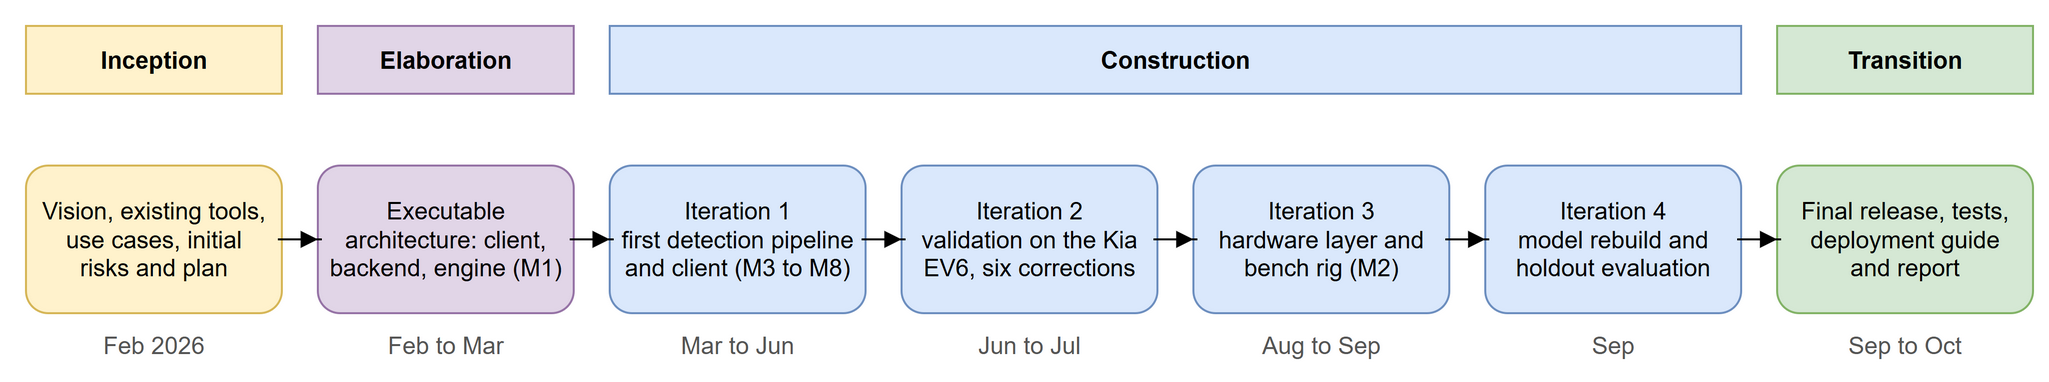
\includegraphics[width=\textwidth]{project_timeline.png}
\caption{Phases and iterations of the Unified Process in the project.}
\label{fig:project-timeline}
\end{figure}

Two rules applied to every iteration. A claim about the system was accepted only once shown on real data, and a defect was considered fixed only once the same test, run again, gave the expected result. As the only developer, we did not reproduce the roles of a team; each iteration ended with a review of its increment against its use cases before the next one started.

\subsection{Modelling language and tools}

The models of this report follow the \gls{uml}~\cite{omg2017uml}. The following diagrams are used:

\begin{itemize}
    \item \textbf{Use case diagram:} It shows the actors of the system and the services the system offers them.
    \item \textbf{Activity diagram:} It shows the flow of actions of a use case, with its decisions, divided between the actors and the system.
    \item \textbf{Class diagram:} It shows the classes of the software, with their attributes, their operations and the relations between them. The domain model, a class diagram of the concepts of the problem without software details, and the data model, which describes the tables of the database, are drawn in the same notation.
    \item \textbf{Component diagram:} It shows the parts of the system and the interfaces through which they depend on each other.
    \item \textbf{Deployment diagram:} It shows the machines and the processes on which the components run, and how they communicate.
    \item \textbf{Sequence diagram:} It shows, for one scenario, the numbered messages exchanged over time between an actor and the boundary, control and entity objects of the system.
    \item \textbf{State diagram:} It shows the states an object goes through and the events that move it from one state to another.
\end{itemize}

The diagrams were drawn with draw.io from a script that keeps every diagram in a file that can be edited. The source code was versioned with Git and GitHub, and the report was typeset with \LaTeX.

\section*{Conclusion}
\addcontentsline{toc}{section}{Conclusion}

This chapter presented the host company, the context of the project, the existing solutions and their limits, the problem and the solution we propose, its objectives, and the Unified Process that organised the work. The next chapter presents the inception phase: the capture of the requirements.

\chapter{Inception: Requirements Capture}
\label{chap:inception}

\section{Introduction}

The inception phase turns the objectives of Chapter~\ref{chap:framework} into requirements. This chapter identifies the actors, states the functional and non functional requirements, builds the use case model that drives the iterations, lists the initial risks, and plans the work by phase and iteration.

\section{Actors}
\label{sec:actors}

An actor is a role played outside the system that interacts with it. CANvisionNative has three:

\begin{itemize}
    \item \textbf{Analyst (main actor).} A BMS engineer or tester who imports logs, starts replays and live sessions, reviews the alerts, asks for explanations, exports reports and configures the platform.
    \item \textbf{Vehicle or \gls{can} bus (secondary actor).} An external system that sends frames on the bus; it is the source of the traffic in a live session, through a \gls{can} adapter.
    \item \textbf{\gls{llm} provider (secondary actor).} An external service that writes the natural language text of an explanation: Google Gemini in the cloud, or a local Ollama model.
\end{itemize}

The backend of CANvisionNative is not an actor: it is part of the system under design, together with the desktop client.

\section{Functional requirements}
\label{sec:fr}

Table~\ref{tab:fr} groups the functional requirements by theme and gives each one a priority: \emph{must} for the requirements without which the platform has no purpose, \emph{should} for those expected in the final release, and \emph{could} for those that are useful but not essential.

\begin{table}[H]
\centering
\footnotesize
\caption{Functional requirements, by theme and priority.}
\label{tab:fr}
\begin{tabularx}{\textwidth}{|P{1.0cm}|Y|P{1.4cm}|}
\hline
\textbf{ID} & \textbf{Requirement} & \textbf{Priority} \\
\hline
\multicolumn{3}{|l|}{\textbf{Input and vehicle}} \\
\hline
FR1 & Import a recorded log in \gls{csv}, \gls{mf4}, Vector (.asc), candump (.log) or PCAN text (.txt) format, and convert it into one common frame stream made of a timestamp, an identifier and a payload. & Must \\
\hline
FR2 & Let the analyst choose the vehicle that produced the log, so that the matching trained model scores the frames and the matching \gls{dbc} file, when one exists, decodes them. & Must \\
\hline
FR12 & For a loaded log, show which signals it carries (the decoded signals when a \gls{dbc} file exists, otherwise the most active raw payload bytes, marked as not decoded) and describe the dataset: its size, its duration, and whether the selected model was trained or tested on it. & Should \\
\hline
FR13 & Show, for every vehicle model, whether it has been evaluated on a recording kept out of its training, and refuse an analysis with a model whose files cannot be shown to belong to one training run. & Must \\
\hline
\multicolumn{3}{|l|}{\textbf{Analysis}} \\
\hline
FR3 & Replay the imported frames in order, at a speed chosen by the analyst (0.5, 1, 2, 4 or 8 times real time, or 32 times as the maximum), and show the progress of the replay. & Must \\
\hline
FR4 & Score every frame for which a model exists and flag the frames whose score passes the calibrated threshold of that model; report the frames that cannot be scored as unresolved, with the reason, instead of counting them as normal; complement the model score with timing, payload and persistence checks. & Must \\
\hline
FR5 & Give each alert a severity level derived from its score. & Must \\
\hline
\multicolumn{3}{|l|}{\textbf{Explanation and reporting}} \\
\hline
FR6 & Explain any alert on request, in natural language, with the dominant signal, the likely cause and a recommended action. & Must \\
\hline
FR7 & Export the alert list as a \gls{csv} file and as a formatted PDF report. & Must \\
\hline
\multicolumn{3}{|l|}{\textbf{Live operation}} \\
\hline
FR8 & Generate a simulated live \gls{can} stream, including a simulated anomaly burst, to test the detection pipeline without a vehicle. & Could \\
\hline
FR9 & Connect to a physical \gls{can} adapter supported by python-can (for example a serial adapter using the slcan protocol, a PEAK PCAN adapter or SocketCAN) and send the received frames into the same runtime engine as replay; offer the live session only when a USB device is detected. & Should \\
\hline
FR10 & Record a live or simulated session to a log file, optionally with an injected and labelled anomaly, for later replay or training. & Could \\
\hline
\multicolumn{3}{|l|}{\textbf{Configuration}} \\
\hline
FR11 & Let the analyst set the key of the \gls{llm} provider, the hardware settings and an alert threshold, and keep these settings between sessions. & Should \\
\hline
\end{tabularx}
\end{table}

\section{Non functional requirements}
\label{sec:nfr}

Table~\ref{tab:nfr} classifies the non functional requirements with the \gls{furps} model.

\begin{table}[H]
\centering
\small
\caption{Non functional requirements, classified with FURPS+.}
\label{tab:nfr}
\begin{tabularx}{\textwidth}{|P{2.4cm}|P{1.1cm}|Y|}
\hline
\textbf{Category} & \textbf{ID} & \textbf{Requirement} \\
\hline
Usability & NFR3 & An analyst without a background in machine learning shall be able to import a log, read the alert list and understand the explanation of an alert without external documentation. \\
\hline
\multirow{2}{2.4cm}{Reliability} & NFR2 & A detection defect shall be shown and corrected with concrete evidence, never by tuning a threshold until the numbers look better. \\
\cline{2-3}
 & NFR6 & If the \gls{llm} provider cannot be reached, the system shall still produce a rule based explanation instead of failing. \\
\hline
Performance & NFR1 & An offline analysis of a recording of several hundred thousand frames shall finish in a few minutes on a standard desktop computer; live scoring shall keep up with the bus in real time. \\
\hline
\multirow{2}{2.4cm}{Supportability} & NFR4 & Every supported log format shall enter the detection pipeline through the same frame representation, so that the results do not depend on the format used to record the data. \\
\cline{2-3}
 & NFR5 & Adding a vehicle shall only require a \gls{dbc} file and a trained model folder that passes the promotion checks, without any change to the detection engine. \\
\hline
Constraints (+) & NFR7 & The desktop client shall run on Windows 10 or 11 with .NET Framework 4.8 and \gls{wpf}; the backend shall run as a local Python process (3.11 or later) that exposes a \gls{rest} \gls{api} on the same machine; only live capture needs extra hardware, a \gls{can} adapter supported by python-can. \\
\hline
\end{tabularx}
\end{table}

\Needspace{580pt}% keep the heading with its float
\section{Use case model}
\label{sec:usecases}

\subsection{Global use case diagram}

Figure~\ref{fig:usecase} shows the use case diagram. Replaying a log, running a live simulation and connecting the hardware include \emph{Detect anomaly}, because the three input modes feed the same runtime engine. Selecting a vehicle includes \emph{Check model status}, since a model is only used once its status allows it. \emph{Request explanation} is an optional extension of \emph{Review alerts}, and the only use case that involves the \gls{llm} provider.

\begin{figure}[H]
\centering
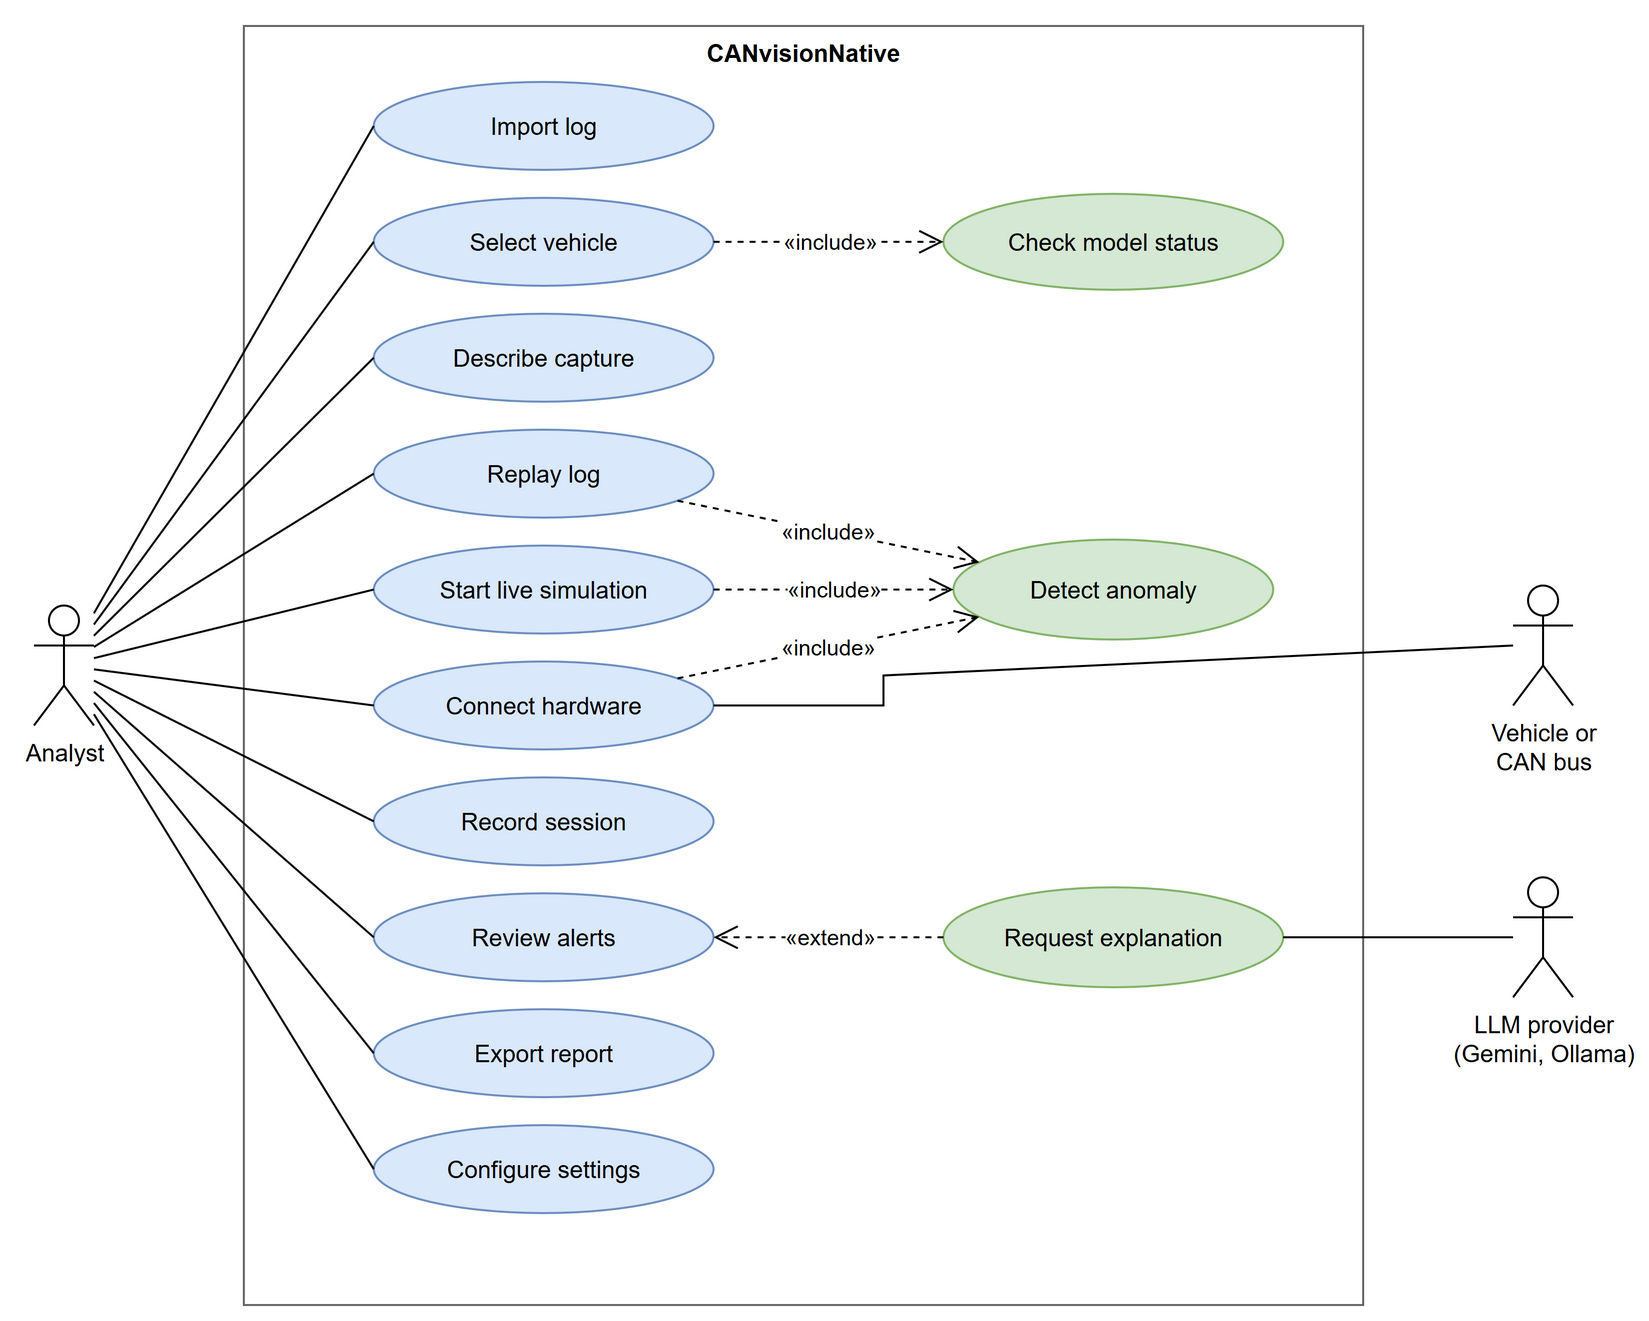
\includegraphics[width=\textwidth]{usecase.png}
\caption{Use case diagram of CANvisionNative.}
\label{fig:usecase}
\end{figure}

\Needspace{446pt}% keep the text with its float
Table~\ref{tab:usecase-table} summarises the use cases and the requirements they cover.

\begin{table}[H]
\centering
\small
\caption{Summary of the use cases.}
\label{tab:usecase-table}
\begin{tabularx}{\textwidth}{|P{3.3cm}|Y|P{1.7cm}|}
\hline
\textbf{Use case} & \textbf{Description} & \textbf{Req.} \\
\hline
Import log & The analyst selects a log file; the system recognises its format and converts it into the common frame stream. & FR1 \\
\hline
Select vehicle & The analyst chooses the vehicle model used to score the log and the \gls{dbc} file used to decode it. & FR2 \\
\hline
Check model status & The system tells whether the chosen model may be used offline or live, and refuses it otherwise. & FR13 \\
\hline
Describe capture & The system shows the signals of the capture and a plain description of the dataset. & FR12 \\
\hline
Replay log & The system replays the frame stream at the chosen speed and runs \emph{Detect anomaly} on it. & FR3 \\
\hline
Start live simulation & The system generates a simulated stream, with an optional anomaly burst, and runs \emph{Detect anomaly} on it. & FR8 \\
\hline
Connect hardware & The system reads live frames from a \gls{can} adapter and runs \emph{Detect anomaly} on them. & FR9 \\
\hline
Detect anomaly & The system scores each frame, reports the frames it cannot score, and raises alerts with a severity. & FR4, FR5 \\
\hline
Record session & The system records a live or simulated session to a log file. & FR10 \\
\hline
Review alerts & The analyst browses the alert list and the signals behind a selected alert. & FR4, FR5 \\
\hline
Request explanation & The system explains a selected alert in plain language. & FR6 \\
\hline
Export report & The analyst exports the alert list as a \gls{csv} file or a PDF report. & FR7 \\
\hline
Configure settings & The analyst sets the \gls{llm} key, the hardware parameters and the alert threshold. & FR11 \\
\hline
\end{tabularx}
\end{table}

\Needspace{395pt}% keep the heading with its float
\subsection{Textual descriptions}

Tables~\ref{tab:uc-analyse} to~\ref{tab:uc-hardware} describe the five main use cases in detail: their preconditions, nominal scenario, alternative scenarios and postconditions.

\newcommand{\ucrow}[2]{\textbf{#1} & #2 \\ \hline}

\Needspace{613pt}% keep the text with its float
Table~\ref{tab:uc-analyse} describes the offline analysis of a log: the use case \emph{Import log}, with the use cases \emph{Select vehicle}, \emph{Check model status} and \emph{Detect anomaly} that it includes.

\begin{table}[H]
\centering
\small
\caption{Use case \emph{Import log}, with \emph{Select vehicle}, \emph{Check model status} and \emph{Detect anomaly} (offline analysis).}
\label{tab:uc-analyse}
\begin{tabularx}{\textwidth}{|P{2.6cm}|Y|}
\hline
\ucrow{Actor}{Analyst.}
\ucrow{Preconditions}{The backend is running; a log file in a supported format is available.}
\ucrow{Nominal scenario}{1. The analyst chooses to import a log on the Home screen and selects a file. 2. The system recognises the format and reads the frames into the common frame stream. 3. The system lists the vehicle models with their status. 4. The analyst selects a model and starts the analysis. 5. The system checks that the model may be used offline. 6. The system scores every frame with the model of its identifier, counts the unresolved frames with their reasons, and merges bursts of alerts. 7. The system shows the results on the Dashboard.}
\ucrow{Alternative scenarios}{2a. The file cannot be read: the system shows the reason and the analysis does not start. 5a. The model may not be used offline (held back, not validated or from the first design): the system refuses the analysis with the reason, and the analyst can choose another model.}
\ucrow{Postconditions}{The alerts and the counts of the analysis are available to every screen of the client.}
\ucrow{Requirements}{FR1, FR2, FR4, FR5, FR13.}
\end{tabularx}
\end{table}

Table~\ref{tab:uc-replay} describes the use case \emph{Replay log}, which plays an imported log again through the runtime engine.

\begin{table}[H]
\centering
\small
\caption{Use case \emph{Replay log}.}
\label{tab:uc-replay}
\begin{tabularx}{\textwidth}{|P{2.6cm}|Y|}
\hline
\ucrow{Actor}{Analyst.}
\ucrow{Preconditions}{A log has been imported and a vehicle model selected.}
\ucrow{Nominal scenario}{1. The analyst opens Log Playback, chooses a speed and starts the replay. 2. The system starts a replay process that reads the file with the common parser. 3. The system sends every frame to the runtime engine (\emph{Detect anomaly}). 4. The client follows the progress and shows the flagged spans and the alerts on the timeline. 5. At the end of the file, the system publishes the alerts of the replay so that they can be explained.}
\ucrow{Alternative scenarios}{1a. The analyst pauses, resumes or stops the replay. 3a. A frame that no model can score is counted as unresolved, with its reason.}
\ucrow{Postconditions}{The replay is completed and its alerts are in the alert list.}
\ucrow{Requirements}{FR3, FR4, FR5.}
\end{tabularx}
\end{table}

\Needspace{535pt}% keep the text with its float
Table~\ref{tab:uc-explain} describes the use case \emph{Request explanation}, the only one that involves the \gls{llm} provider.

\begin{table}[H]
\centering
\small
\caption{Use case \emph{Request explanation}.}
\label{tab:uc-explain}
\begin{tabularx}{\textwidth}{|P{2.6cm}|Y|}
\hline
\ucrow{Actors}{Analyst; \gls{llm} provider.}
\ucrow{Preconditions}{An analysis or a replay has produced alerts, which the analyst reviews in Anomaly Intel.}
\ucrow{Nominal scenario}{1. The analyst selects an alert. 2. The system finds the alert in the current session and builds its context. 3. The system sends the context to Gemini. 4. Gemini returns a text. 5. The system shows the summary, the likely cause and the recommendation, with the name of the engine that wrote them.}
\ucrow{Alternative scenarios}{2a. The alert does not belong to the current session: the system returns no explanation. 3a. Gemini cannot be reached: the system asks the local Ollama model. 3b. No language model answers: the system writes a rule based text from the measured values.}
\ucrow{Postconditions}{The explanation is shown; the score, the flag and the severity of the alert are unchanged.}
\ucrow{Requirements}{FR6, NFR6.}
\end{tabularx}
\end{table}

Table~\ref{tab:uc-export} describes the use case \emph{Export report}, which saves the alert list of a session.

\begin{table}[H]
\centering
\small
\caption{Use case \emph{Export report}.}
\label{tab:uc-export}
\begin{tabularx}{\textwidth}{|P{2.6cm}|Y|}
\hline
\ucrow{Actor}{Analyst.}
\ucrow{Preconditions}{An alert list is shown in Anomaly Intel.}
\ucrow{Nominal scenario}{1. The analyst chooses to export the list as a PDF report or a \gls{csv} file. 2. The system asks for a file name. 3. The system writes the PDF report (session, summary by severity, identifiers with the most alerts, alerts in time order and explanations) or the \gls{csv} file (one row per alert).}
\ucrow{Alternative scenarios}{2a. The analyst cancels: nothing is written.}
\ucrow{Postconditions}{The report or the file is saved where the analyst chose.}
\ucrow{Requirements}{FR7.}
\end{tabularx}
\end{table}

\Needspace{304pt}% keep the text with its float
Table~\ref{tab:uc-hardware} describes the use case \emph{Connect hardware}, which starts a live capture from a \gls{can} adapter.

\begin{table}[H]
\centering
\small
\caption{Use case \emph{Connect hardware} (live capture).}
\label{tab:uc-hardware}
\begin{tabularx}{\textwidth}{|P{2.6cm}|Y|}
\hline
\ucrow{Actors}{Analyst; vehicle or \gls{can} bus.}
\ucrow{Preconditions}{The backend is running and a USB \gls{can} adapter is plugged in.}
\ucrow{Nominal scenario}{1. The analyst starts a live session on the Home screen. 2. The system opens the hardware setup. 3. The analyst chooses the interface, the port, the bitrate and the vehicle model, and connects. 4. The system builds a live engine for the chosen model and opens the adapter. 5. The system decodes each received frame with the \gls{dbc} file of the vehicle, when there is one, and scores it (\emph{Detect anomaly}). 6. The live screens show the signals and the alerts. 7. The analyst disconnects and the scoring stops.}
\ucrow{Alternative scenarios}{1a. No USB device is detected: the live session stays locked. 4a. The model is held back or unknown: the connection is refused with the reason. 5a. No frame arrives for a few seconds: the link is reported as lost.}
\ucrow{Postconditions}{The adapter is released; the alerts of the session remain available.}
\ucrow{Requirements}{FR2, FR9.}
\end{tabularx}
\end{table}

\Needspace{445pt}% keep the text with its float
\Needspace{431pt}% keep the heading with its float
\subsection{Activity diagram}

Figure~\ref{fig:activity-replay} shows the flow of the main use case, from the import of a log to the display of its results and their replay.

\begin{figure}[H]
\centering
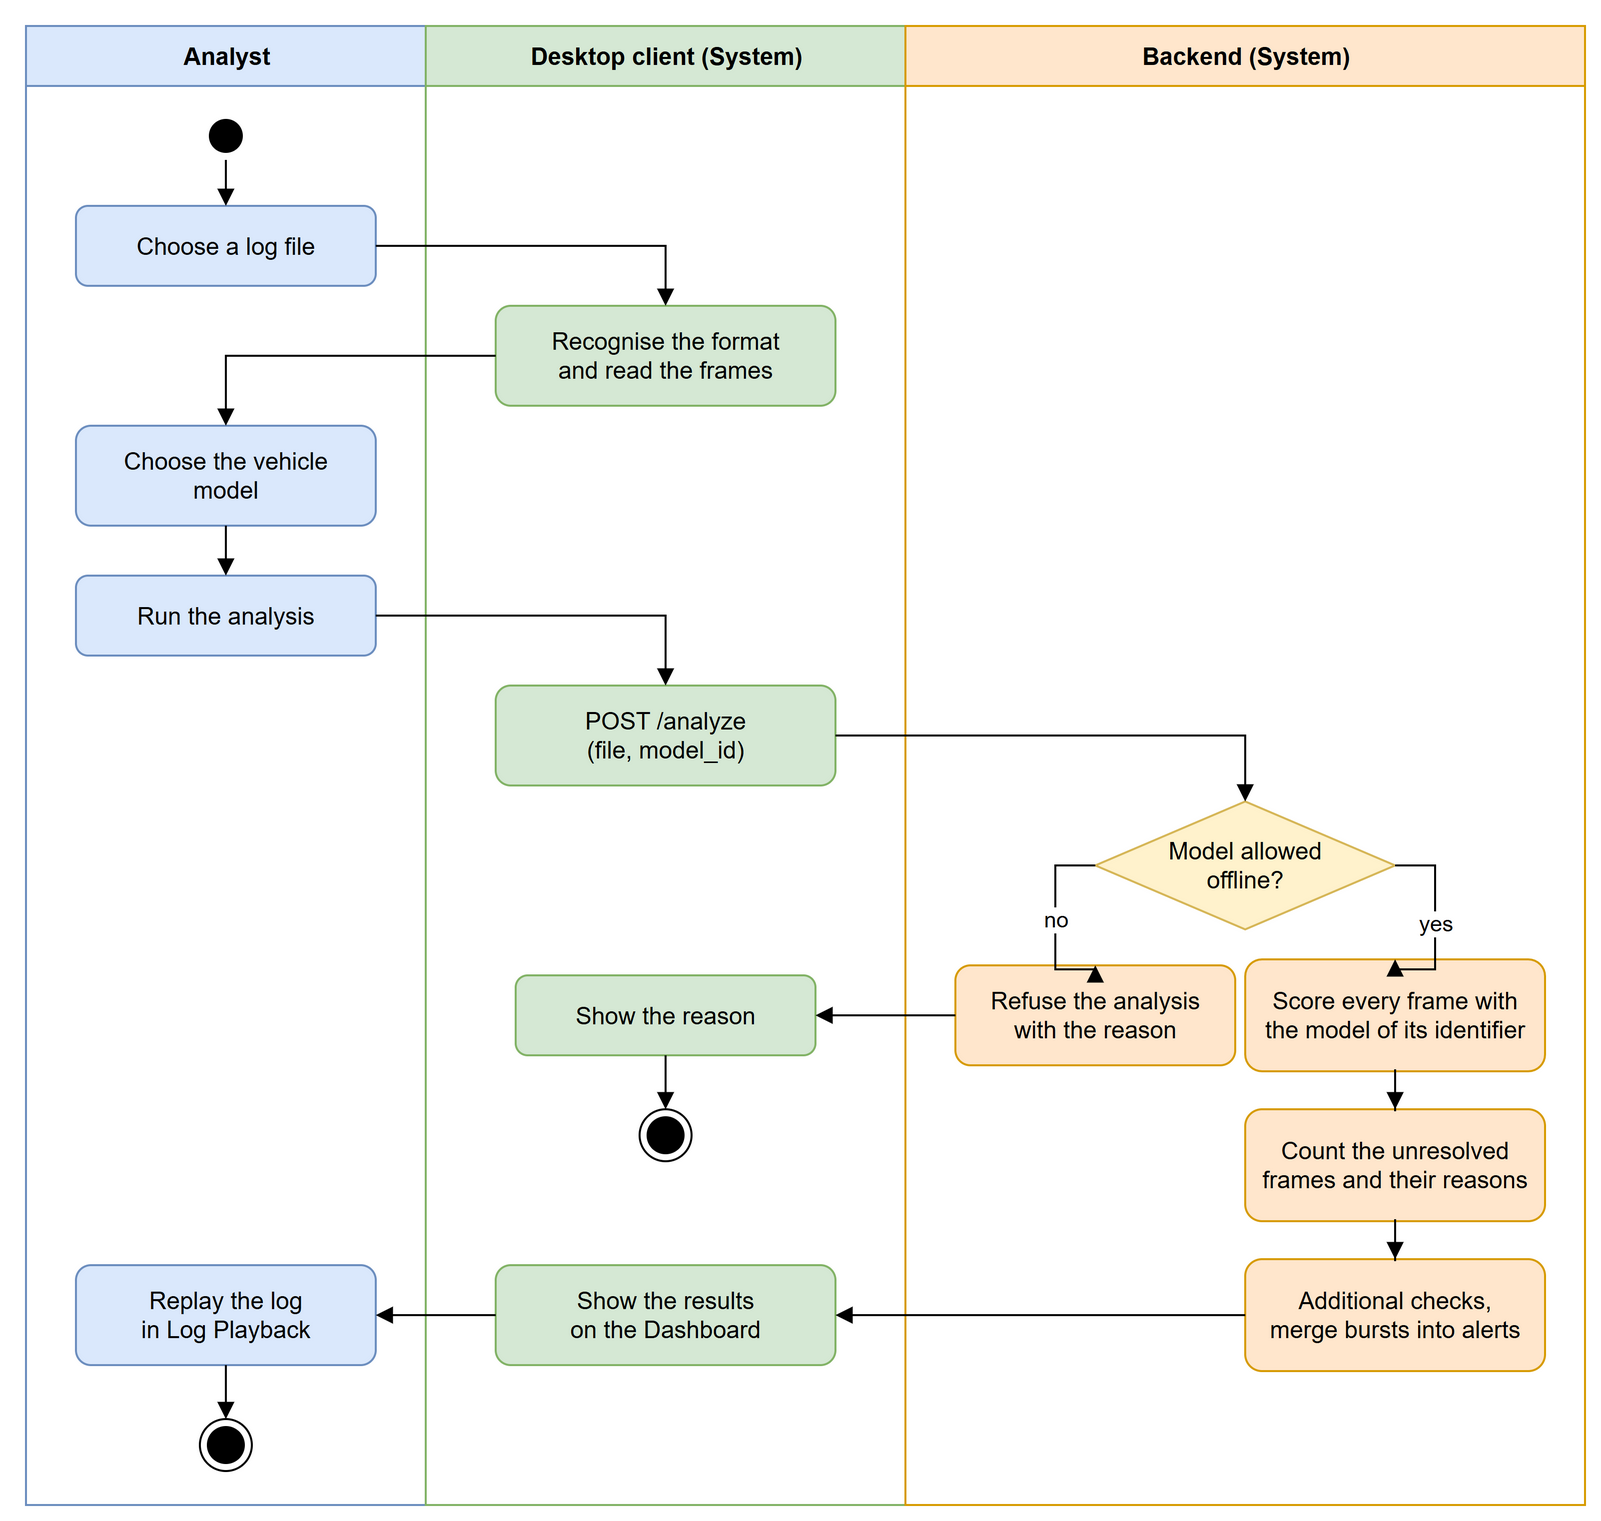
\includegraphics[width=0.74\textwidth]{activity_replay.png}
\caption{Activity diagram: importing, analysing and replaying a log.}
\label{fig:activity-replay}
\end{figure}

\Needspace{632pt}% keep the text with its float
\Needspace{622pt}% keep the heading with its float
\section{Initial risk list}
\label{sec:risks}

Table~\ref{tab:risks} lists the risks identified during inception, with their probability, their impact, the planned mitigation and the iteration that addresses each one. Following the \gls{up}, the iterations were ordered so that the riskiest parts were tackled early; what actually happened to each risk is discussed in the general conclusion.

\begin{table}[H]
\centering
\small
\caption{Initial risk list.}
\label{tab:risks}
\begin{tabularx}{\textwidth}{|P{3.0cm}|P{1.85cm}|P{1.3cm}|Y|P{2.05cm}|}
\hline
\textbf{Risk} & \textbf{Probability} & \textbf{Impact} & \textbf{Planned mitigation} & \textbf{Iteration} \\
\hline
R1. No vehicle available to test live capture & High & Medium & One runtime engine shared by replay, simulation and live capture, so that live capture differs only by its transport; a bench rig to test that transport. & Elaboration, iteration 3 \\
\hline
R2. \gls{llm} provider unavailable or not authenticated & Medium & Low & A chain of providers: Gemini, then a local Ollama model, then a rule based text. & Iteration 1 \\
\hline
R3. Wrong model applied to a vehicle & Medium & High & An explicit choice of the model, checked end to end on a real recording. & Iterations 2 and 4 \\
\hline
R4. A model that does not generalise to new recordings & Medium & High & Evaluate every model on a recording kept out of its training before it enters production. & Iteration 4 \\
\hline
R5. Live scoring too slow for buses with a high frame rate & Medium & Medium & An offline analysis path for whole recordings; measure the throughput of the live path. & Iteration 4 \\
\hline
R6. Too many alerts, so the analyst stops trusting them & Medium & High & Thresholds calibrated on the training data, persistence checks, and unscored frames reported apart instead of counted. & Iterations 2 and 4 \\
\hline
R7. Log formats read differently by different paths & Medium & Medium & One common parser and one frame representation for every path. & Iterations 1 and 2 \\
\hline
R8. Explanation shown for the wrong alert & Low & High & Tie each explanation to the alert of the current session, and test explanations across datasets of different vehicles. & Iteration 2 \\
\hline
\end{tabularx}
\end{table}

\section{Project plan by phase and iteration}
\label{sec:plan}

Figure~\ref{fig:gantt} shows the plan of the project from February to October 2026, organised by phase of the \gls{up}. The whole project was carried out alongside a full time QA position in the BMS team. Inception took the first week of February, while the work on the executable architecture of M1 was starting; the boundaries of the other periods also overlap slightly, because a milestone was being finished while the next one was starting.

\begin{figure}[H]
\centering
\resizebox{\textwidth}{!}{%
\begin{ganttchart}[
    time slot format=isodate,
    hgrid,
    vgrid=false,
    bar/.append style={fill=cyan!60},
    group/.append style={fill=black!70},
    bar height=0.6,
    group height=0.35,
    bar label font=\small,
    group label font=\small\bfseries,
    title label font=\small,
    y unit chart=0.62cm,
    y unit title=0.6cm,
    x unit=0.055cm
]{2026-02-01}{2026-10-31}
\gantttitlecalendar{month=shortname} \\
\ganttgroup{Inception}{2026-02-01}{2026-02-07} \\
\ganttbar{Vision, use cases, risks, plan}{2026-02-01}{2026-02-07} \\
\ganttgroup{Elaboration}{2026-02-02}{2026-03-13} \\
\ganttbar{M1: live foundation (architecture)}{2026-02-02}{2026-03-13} \\
\ganttgroup{Construction, iteration 1}{2026-03-02}{2026-06-22} \\
\ganttbar{M3: training for several driving states}{2026-03-02}{2026-04-24} \\
\ganttbar{M4: explanation engine}{2026-04-06}{2026-06-19} \\
\ganttbar{M5: real time charts}{2026-05-04}{2026-06-18} \\
\ganttbar{M6: session recording}{2026-05-25}{2026-06-21} \\
\ganttbar{M8: offline and live decoding}{2026-05-18}{2026-06-22} \\
\ganttbar{M7: integration}{2026-06-08}{2026-06-22} \\
\ganttgroup{Construction, iteration 2}{2026-06-22}{2026-07-31} \\
\ganttbar{Validation on real data}{2026-06-22}{2026-07-17} \\
\ganttbar{Correction and new validation}{2026-07-06}{2026-07-31} \\
\ganttgroup{Construction, iteration 3}{2026-08-10}{2026-09-12} \\
\ganttbar{M2: hardware layer and bench rig}{2026-08-10}{2026-09-12} \\
\ganttgroup{Construction, iteration 4}{2026-09-14}{2026-09-26} \\
\ganttbar{Model rebuild and holdout evaluation}{2026-09-14}{2026-09-26} \\
\ganttgroup{Transition}{2026-09-21}{2026-10-16} \\
\ganttbar{Final tests, deployment guide, report}{2026-09-21}{2026-10-16}
\end{ganttchart}%
}
\caption[Project plan by phase and iteration, February to October 2026.]{Project plan by phase and iteration of the Unified Process, February to October 2026 (Gantt chart).}
\label{fig:gantt}
\end{figure}

\section{Conclusion}

The inception phase identified three actors, thirteen functional and seven non functional requirements, the use cases that drive the iterations, and the main risks of the project. The next chapter presents the elaboration phase: the analysis and the architecture.

\chapter{Elaboration: Analysis and Architecture}
\label{chap:elaboration}

\section{Introduction}

The elaboration phase analyses the requirements of Chapter~\ref{chap:inception} and builds the architecture on which the construction iterations grow. This chapter says what the system is made of and why: the technical choices, the overall architecture, the analysis model, the dynamic view of the key use cases, the detection architecture, and the framing of the machine learning problem. It ends with the architecture baseline that the phase delivered, and the risks it reduced. How each part was implemented is described in the iterations of Chapter~\ref{chap:construction}.

\section{Technical choices}
\label{sec:tech-used}

Figure~\ref{fig:tech-logos} shows the technologies used in the project.

\begin{figure}[H]
\centering
\begin{tabular}{ccccc}
\techlogo{dotnet.pdf}{C\# / .NET / WPF} & \techlogo{python.pdf}{Python} & \techlogo{fastapi.pdf}{FastAPI} & \techlogo{sqlite.pdf}{SQLite} & \techlogo{scikitlearn.pdf}{scikit-learn} \\[0.45cm]
\techlogo{pandas.pdf}{pandas} & \techlogo{numpy.pdf}{NumPy} & \techlogo{pytest.pdf}{pytest} & \techlogo{googlegemini.pdf}{Google Gemini} & \techlogo{ollama.pdf}{Ollama} \\[0.45cm]
\techlogo{arduino.pdf}{Arduino} & \techlogo{git.pdf}{Git} & \techlogo{github.pdf}{GitHub} & \techlogo{drawio.pdf}{draw.io} & \techlogo{latex.pdf}{\LaTeX} \\
\end{tabular}
\caption[Technologies used in the project.]{Technologies used in the client, the backend, the machine learning, the tests, the bench rig and the documentation.}
\label{fig:tech-logos}
\end{figure}

The role of each technology is the following:

\begin{itemize}
    \item \textbf{C\# and WPF (.NET Framework 4.8):} \gls{wpf} is the Microsoft framework for native Windows desktop applications, used here with the \gls{mvvm} pattern and the CommunityToolkit.Mvvm library. Its data binding suits a client with many screens and charts, and .NET Framework 4.8 was the target platform of the project.
    \item \textbf{Python, FastAPI, pandas and NumPy:} FastAPI~\cite{fastapi} builds typed \gls{rest} APIs that document themselves, and it works directly with the Python data libraries used for the machine learning. The backend is served by uvicorn.
    \item \textbf{scikit-learn:} The scikit-learn library~\cite{pedregosa2011scikit} provides the Isolation Forests~\cite{liu2008isolation} of the models and the K-Means~\cite{macqueen1967methods} of the first design. Classical methods covered both needs, so no deep learning framework was required.
    \item \textbf{asammdf, cantools and python-can:} The asammdf library reads ASAM \gls{mf4}~\cite{asam_mdf} logs, cantools decodes frames with a \gls{dbc} file, and python-can~\cite{pythoncan} gives one interface to many physical \gls{can} adapters, including the Arduino bridge of our bench rig.
    \item \textbf{SQLite:} An embedded database without a server, enough for a system that runs on one workstation.
    \item \textbf{Google Gemini and Ollama:} They are used only by the explanation module: Gemini in the cloud, Ollama as a local model that works without an internet connection. When neither is available, a rule based template writes the explanation.
    \item \textbf{Development environment:} Visual Studio for the client, a Python virtual environment for the backend, PDFsharp to build the PDF report in C\#, pytest and xUnit for the automated tests, Git and GitHub to version the project, with the large model files in Git LFS, draw.io for the diagrams and MiKTeX for this report. A Windows workstation served for development, training and validation, and a bench rig of two Arduino boards for live capture.
\end{itemize}

\Needspace{657pt}% keep the heading with its float
\section{Overall architecture}
\label{sec:architecture}

\subsection{Logical view in layers}

CANvisionNative runs as two programs on the same machine, a Windows desktop client and a local Python backend, which talk over \gls{http}, as shown in Figure~\ref{fig:overall-arch} below.

The client only talks to the \gls{api} layer, which sends each request to the detection engine or to the data layer, and calls the explanation engine only when the analyst asks for an explanation. We chose this separation so that the detection could be tested through the \gls{api} without the client.

\begin{figure}[H]
\centering
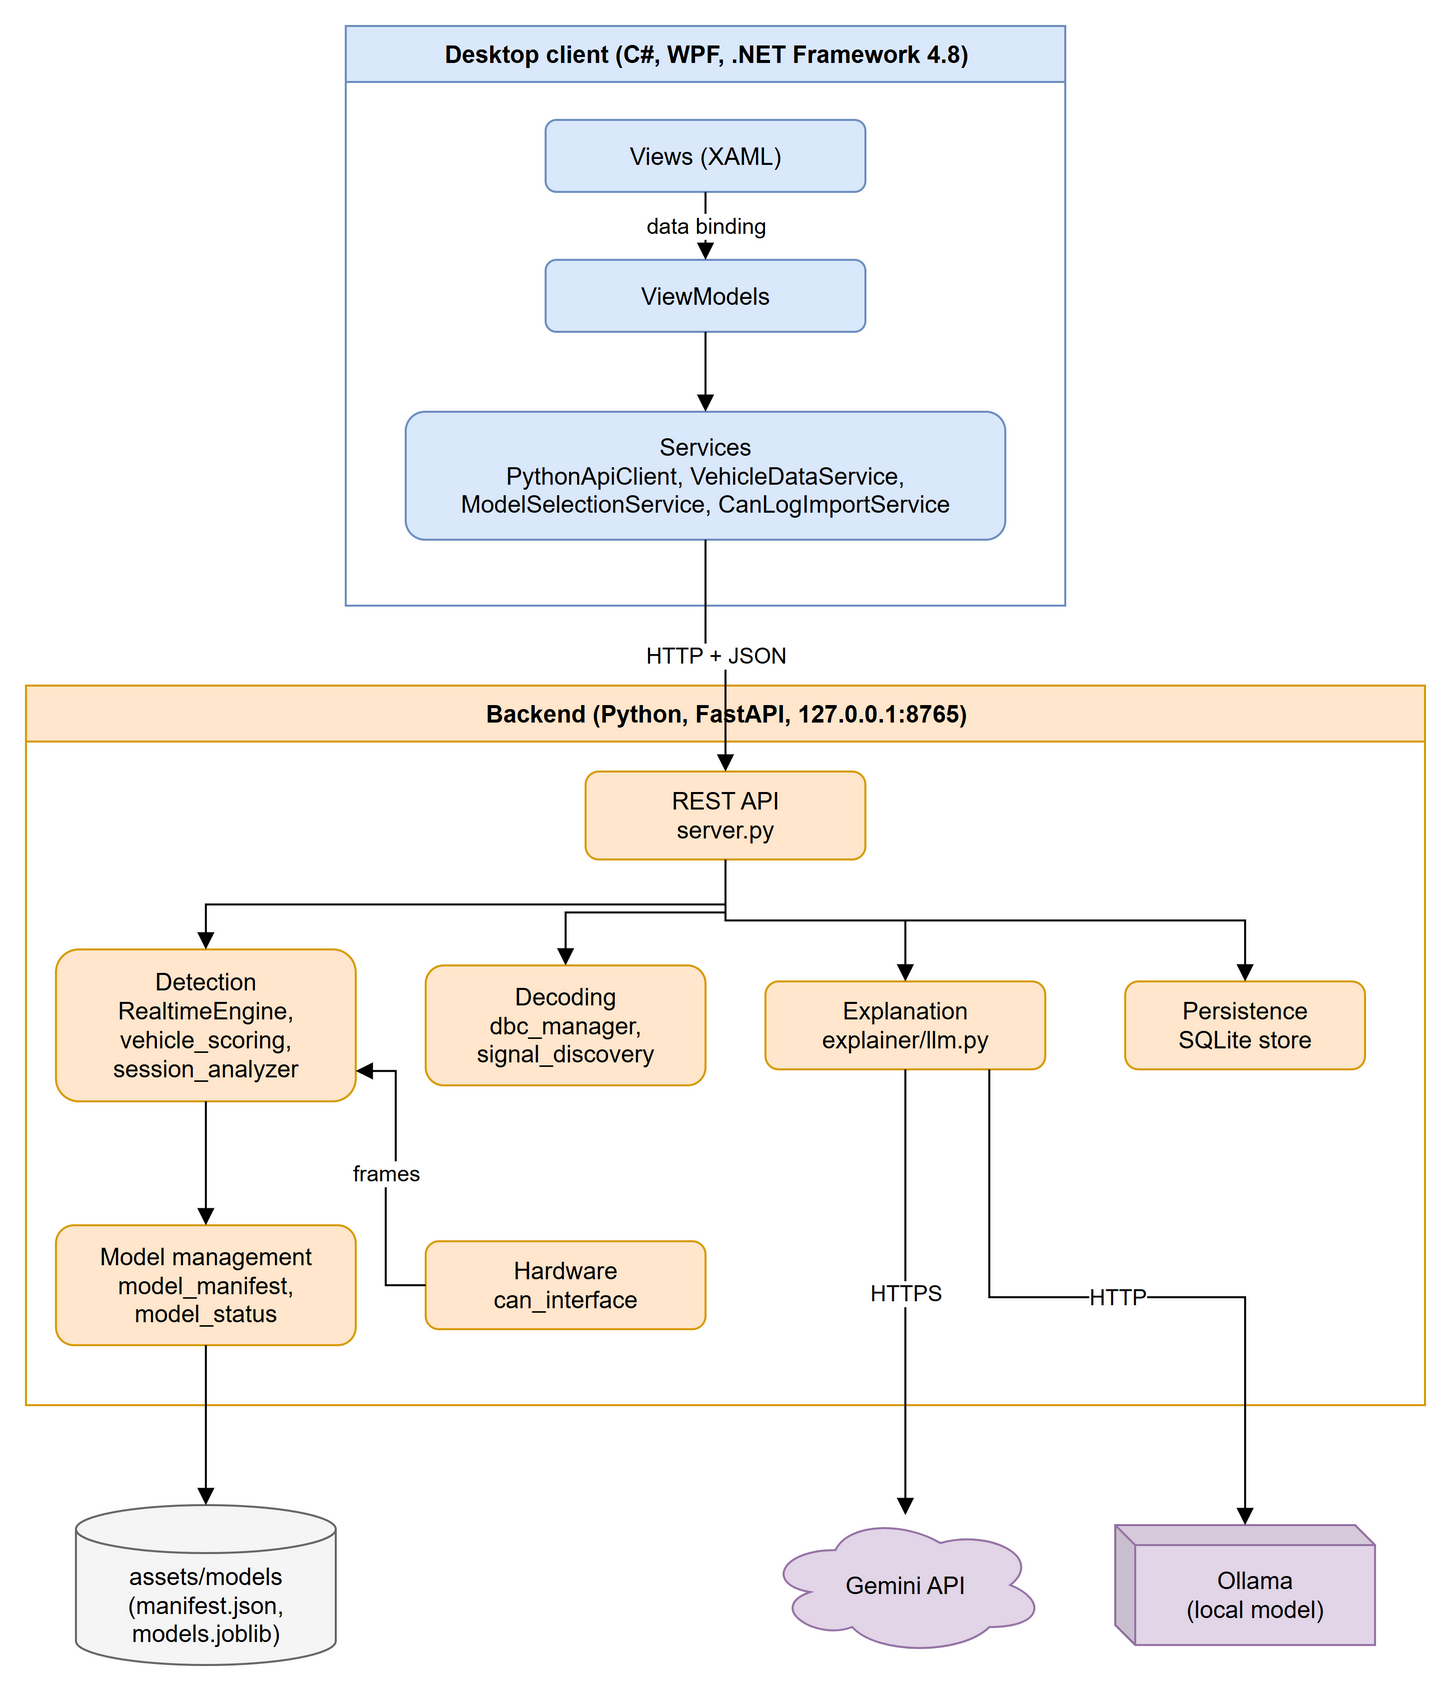
\includegraphics[width=0.8\textwidth]{architecture_overall.png}
\caption{Overall layered architecture of CANvisionNative.}
\label{fig:overall-arch}
\end{figure}

\subsection{Components}
\label{sec:design-backend}

Figure~\ref{fig:components} shows the components and their dependencies. In the client, the views are bound to their ViewModels, which go through a layer of client services to reach the backend. In the backend, the \gls{rest} \gls{api} is the only entry point. It starts the offline analyzer for whole recordings, the replay runner and the hardware interface for frame by frame traffic, and calls the explanation engine and the persistence layer. The replay runner and the hardware interface share the runtime engine, and every component that scores frames obtains its models through the model management component, which reads the model files and their manifests. Long tasks, such as a replay or an offline analysis, run in the background while the client follows their status.

\begin{figure}[H]
\centering
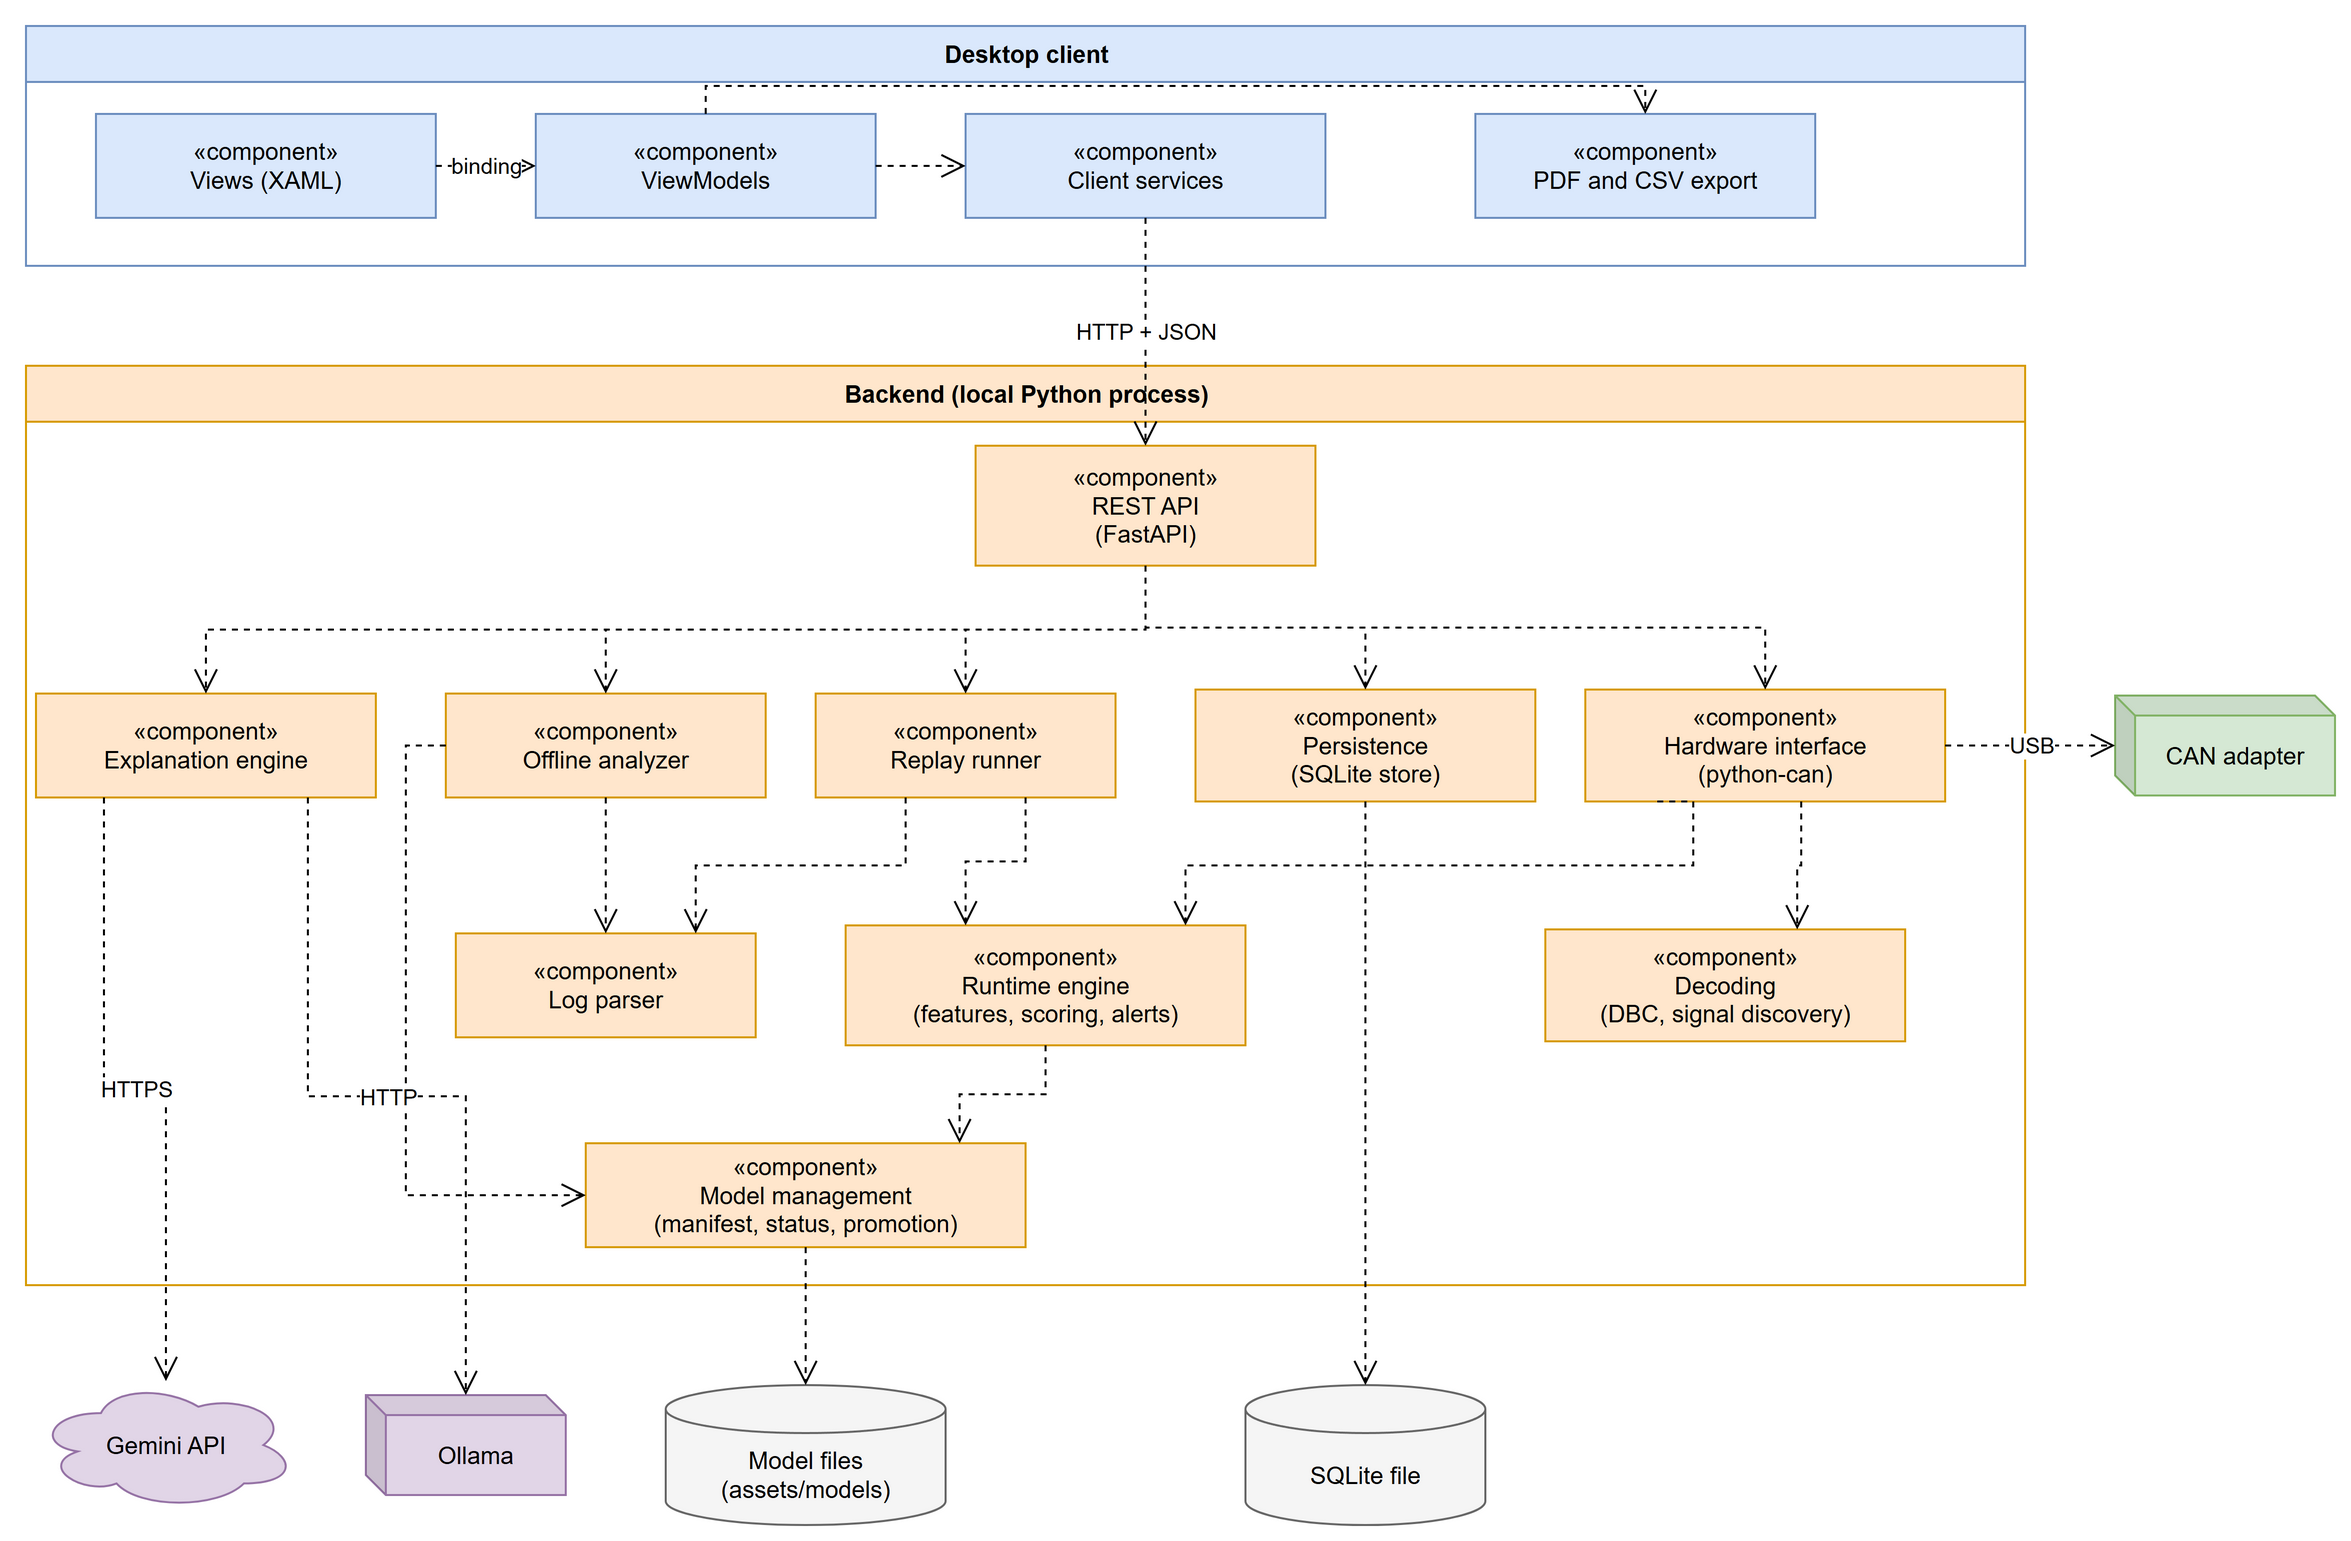
\includegraphics[width=\textwidth]{component_diagram.png}
\caption{Component diagram of the client and the backend.}
\label{fig:components}
\end{figure}

\Needspace{538pt}% keep the heading with its float
\subsection{Client architecture (MVVM)}
\label{sec:design-frontend}

Each screen of the client (Home, Dashboard, Telemetry, Diagnostics, Log Playback, Anomaly Intel and Settings) has a XAML view and its ViewModel; a Hardware Setup screen opens from Home when a live session starts. Two services sit between the ViewModels and the backend (Figure~\ref{fig:frontend-arch}): an \gls{api} client with one method per endpoint, and a data service that keeps the shared state, polls the backend and notifies the screens.

\begin{figure}[H]
\centering
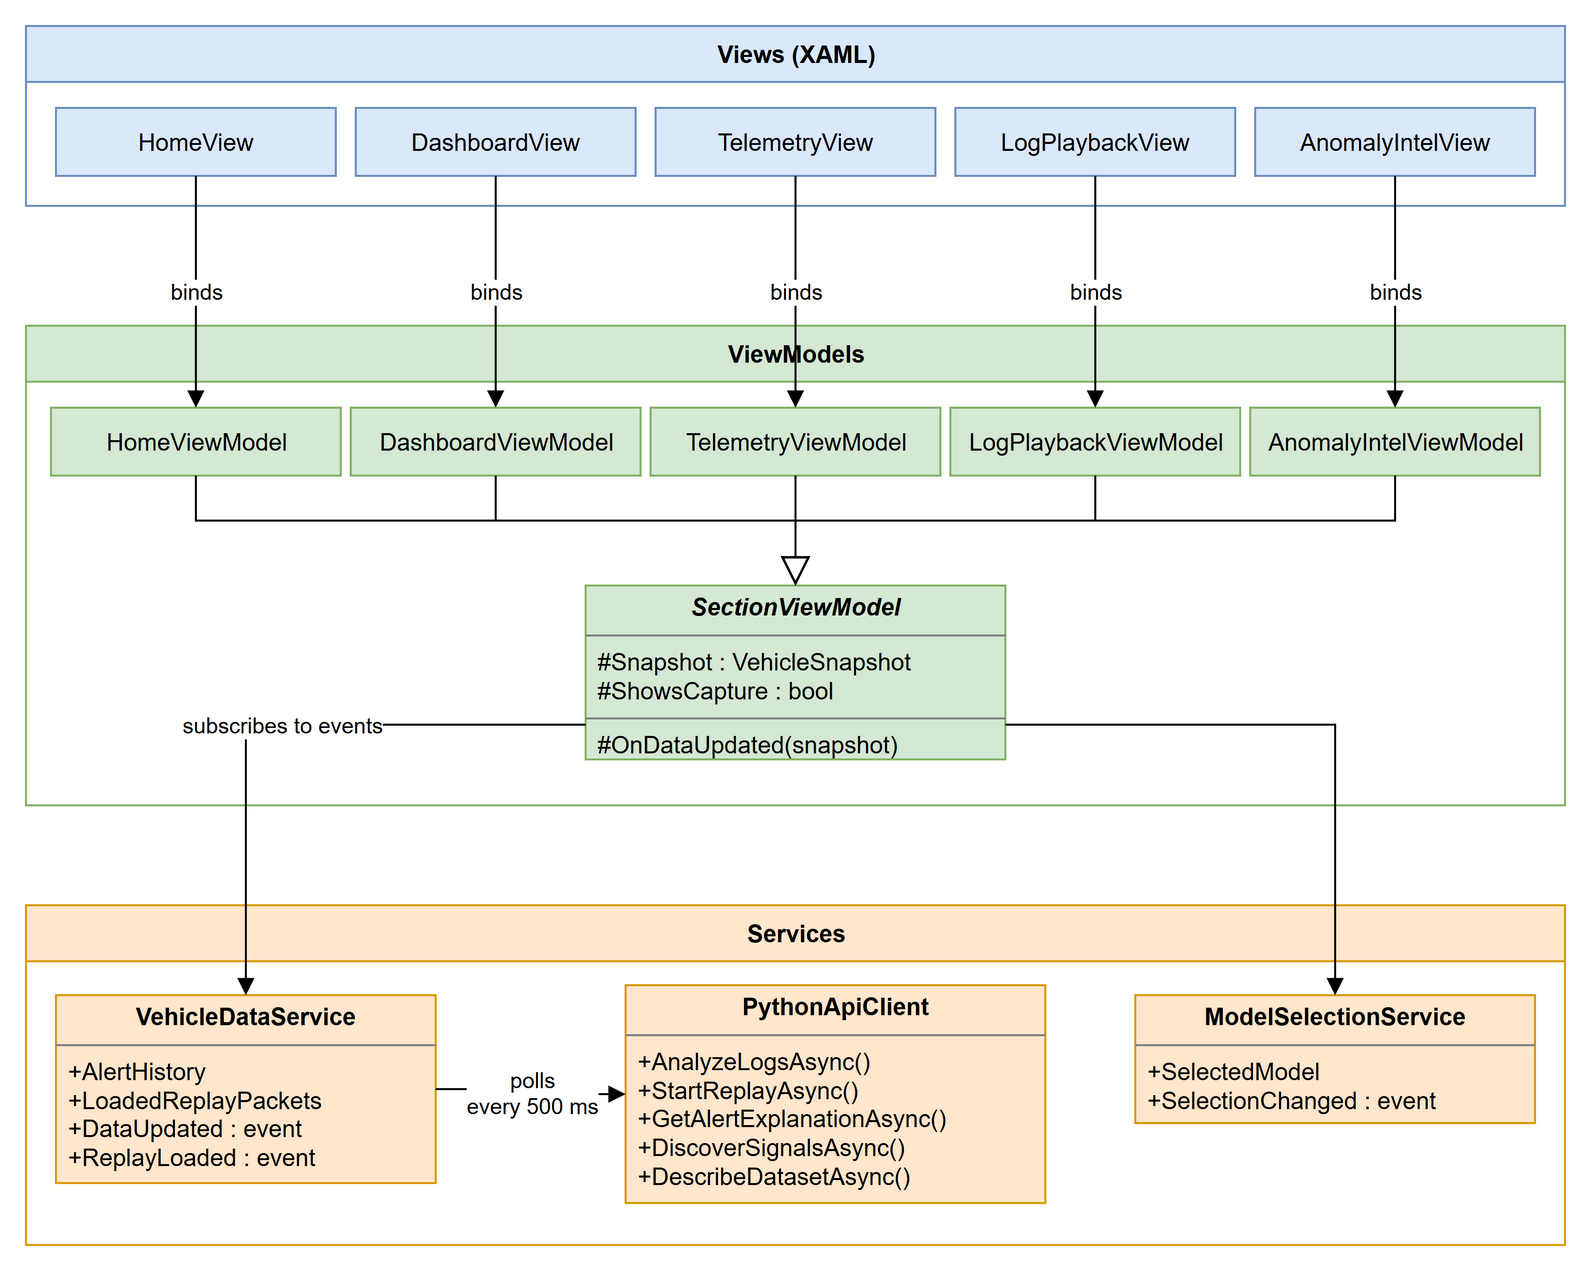
\includegraphics[width=\textwidth]{architecture_frontend.png}
\caption[Frontend architecture of the client.]{Frontend architecture: MVVM views bound to their ViewModels, with two shared services.}
\label{fig:frontend-arch}
\end{figure}

\Needspace{447pt}% keep the text with its float
\Needspace{447pt}% keep the heading with its float
\subsection{Deployment}

Figure~\ref{fig:deployment} shows the deployment. The client and the backend run on the analyst's workstation, next to the SQLite file, the model folder and an optional local Ollama model; Gemini is reached over HTTPS, and the \gls{can} adapter over USB.

\begin{figure}[H]
\centering
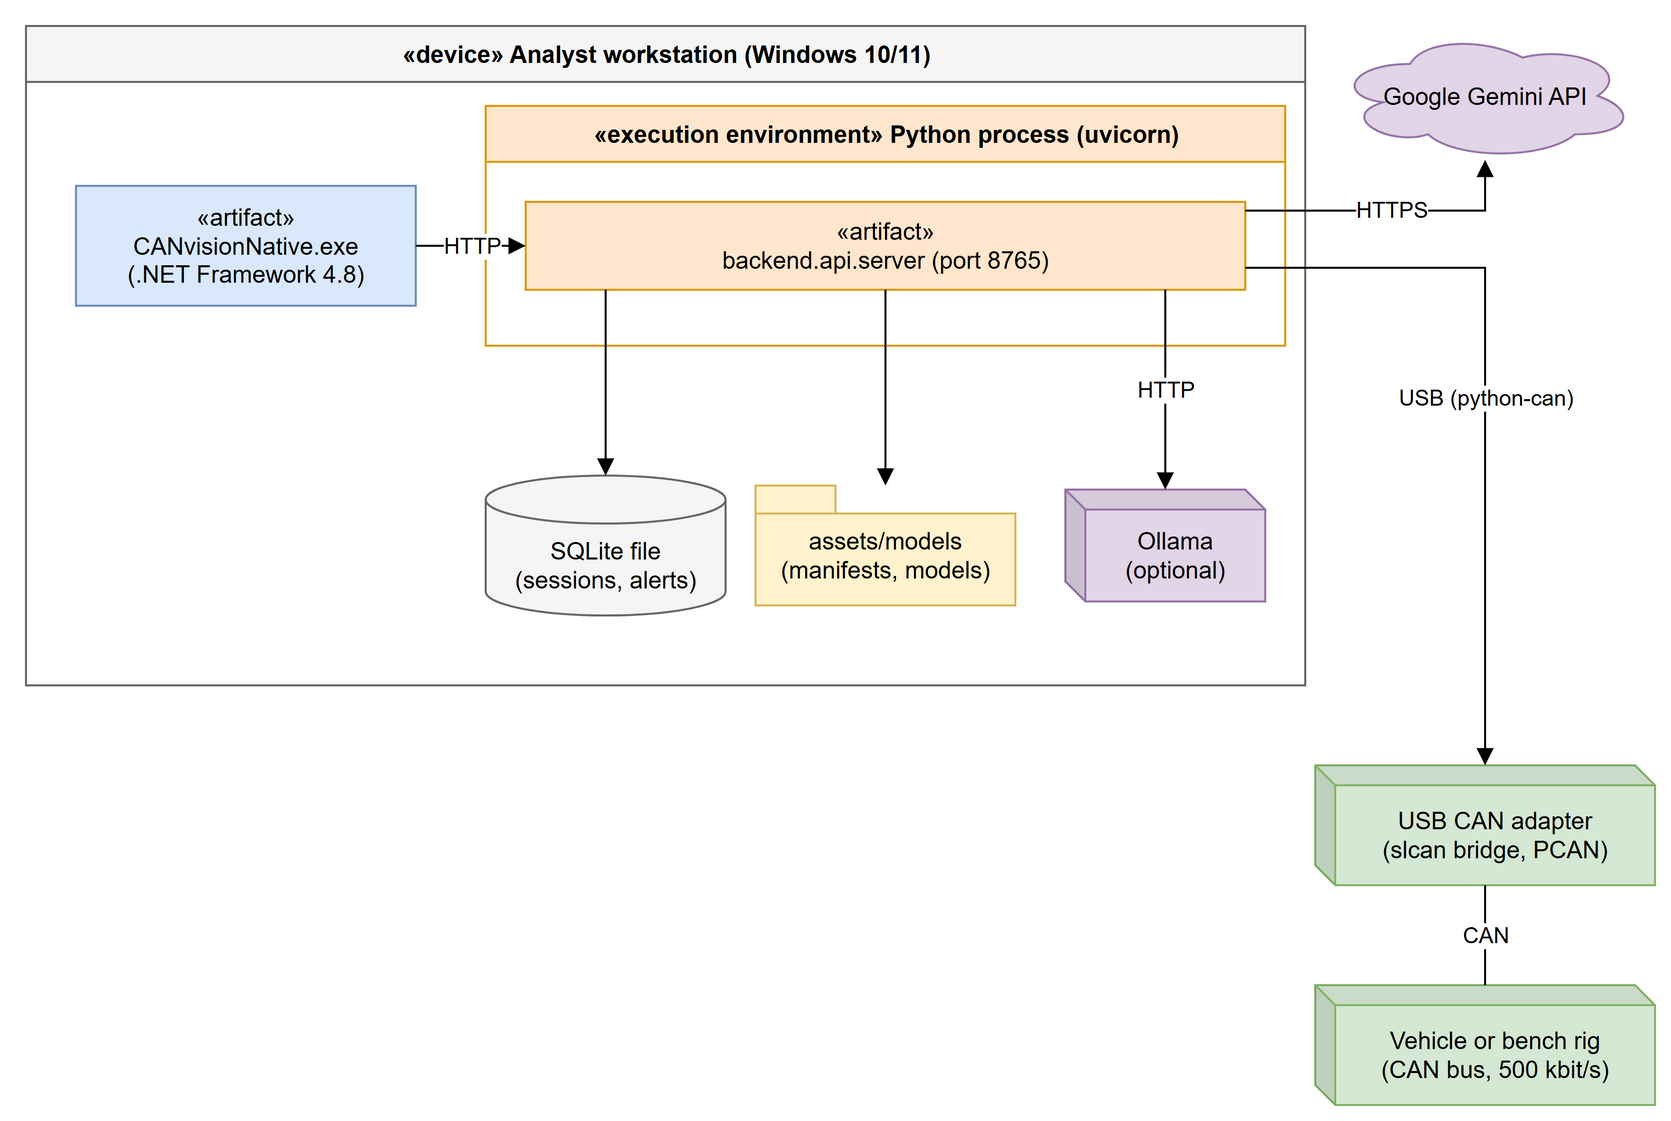
\includegraphics[width=\textwidth]{deployment.png}
\caption[Deployment diagram.]{Deployment diagram: one workstation, with the external \acrshort{llm} and the hardware links.}
\label{fig:deployment}
\end{figure}

\Needspace{631pt}% keep the heading with its float
\section{Analysis model}

\subsection{Domain model}

Figure~\ref{fig:domain-model} shows the concepts of the domain. A \emph{vehicle} may have a \emph{profile}, whose \gls{dbc} files define the \emph{signals} that its frames carry, and a \emph{vehicle model}, made of one \emph{identifier model} per \gls{can} identifier. A \emph{recording} of a vehicle is a sequence of \emph{frames}. A \emph{session}, offline, replay or live, analyses at most one recording with one vehicle model; it counts the frames scored, flagged and unresolved, and produces \emph{alerts}, each of which may receive an \emph{explanation}. A \emph{report} exports one session.

\begin{figure}[H]
\centering
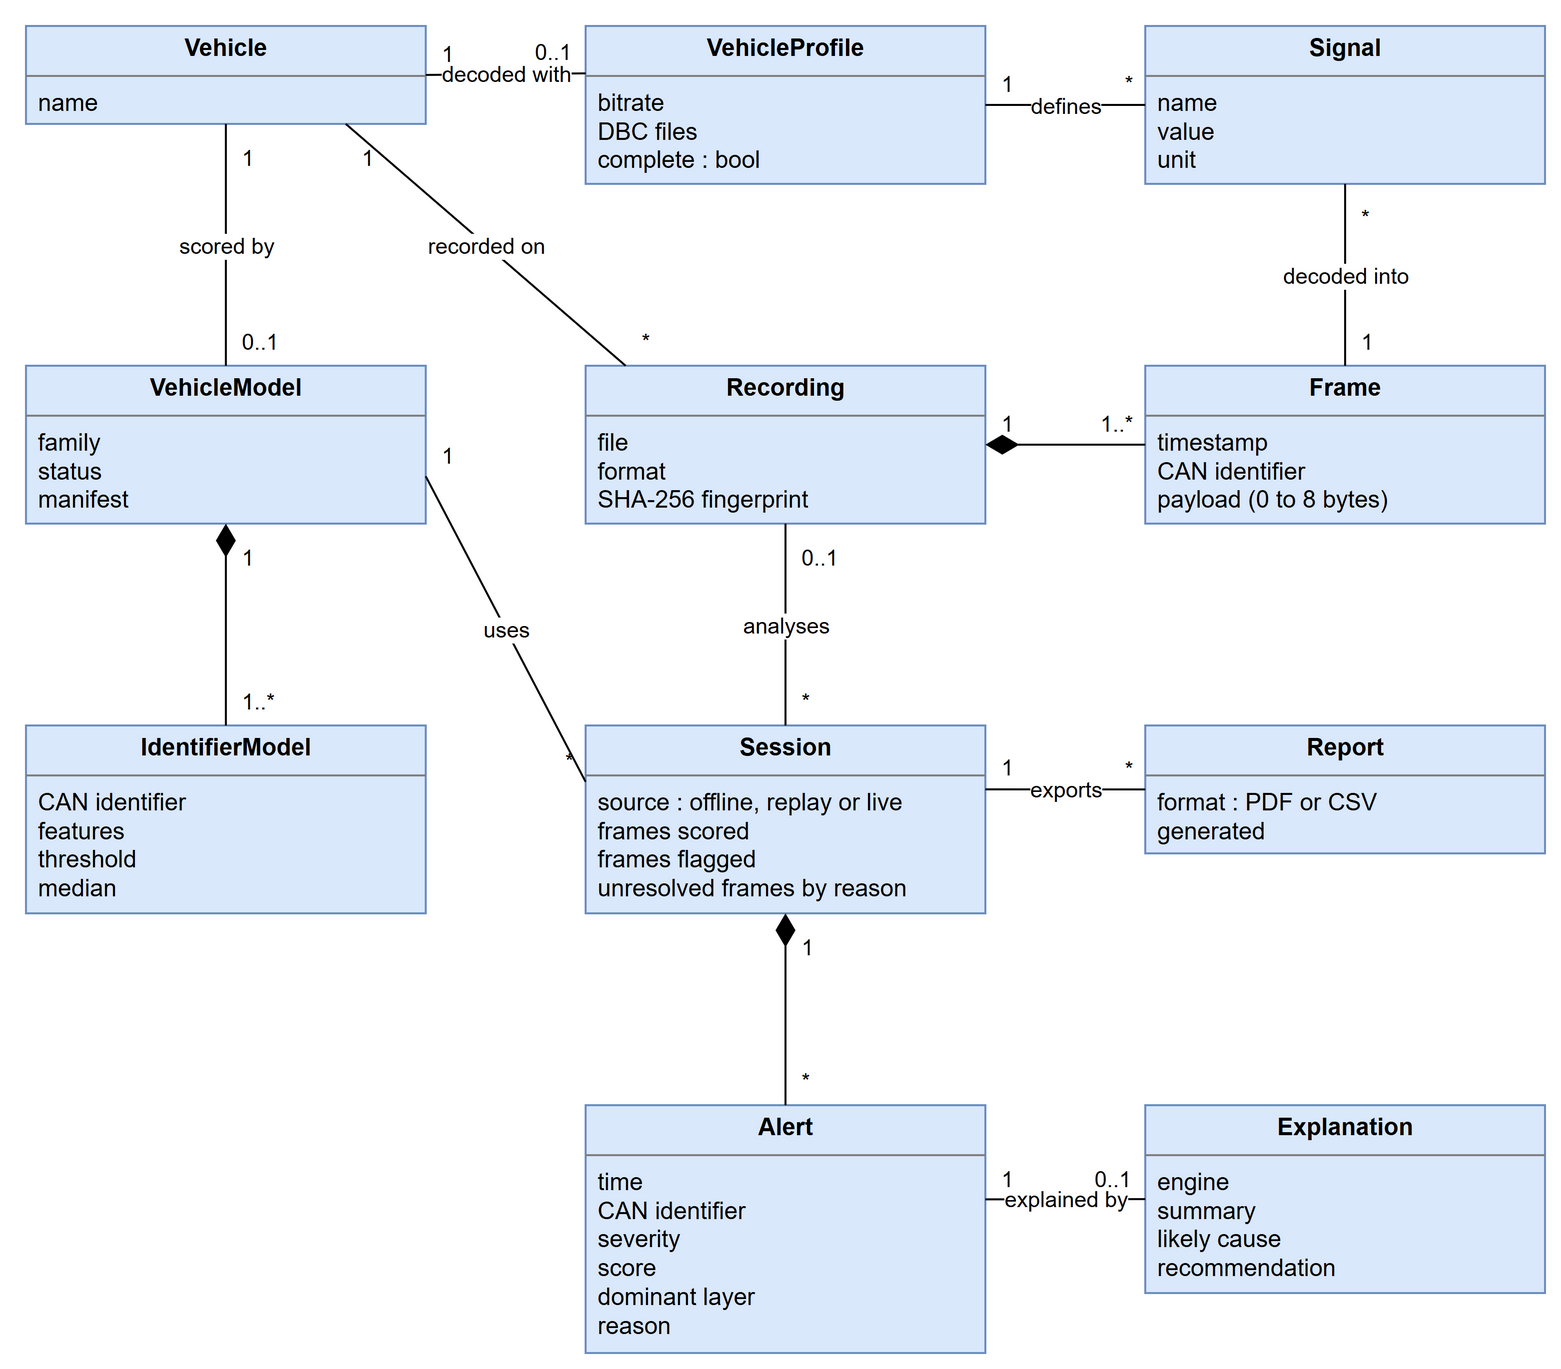
\includegraphics[width=\textwidth]{domain_model.png}
\caption{Domain model of CANvisionNative.}
\label{fig:domain-model}
\end{figure}

\Needspace{555pt}% keep the heading with its float
\subsection{Class diagrams}
\label{sec:class-diagrams}

The class diagrams refine the domain model into the classes of the software, on the backend and on the client side.

Figure~\ref{fig:class-diagram} shows the classes of the detection core of the backend. RealtimeEngine is the single entry point of replay, simulation and live capture; it asks ScoringEngine to combine the layers and, for a vehicle with a final model, its IdModelFamily, loaded from the manifest, for the score of each identifier. The model status resolver decides which model a vehicle may use on each path, and IDSStatistics counts the frames and alerts of a run.

\begin{figure}[H]
\centering
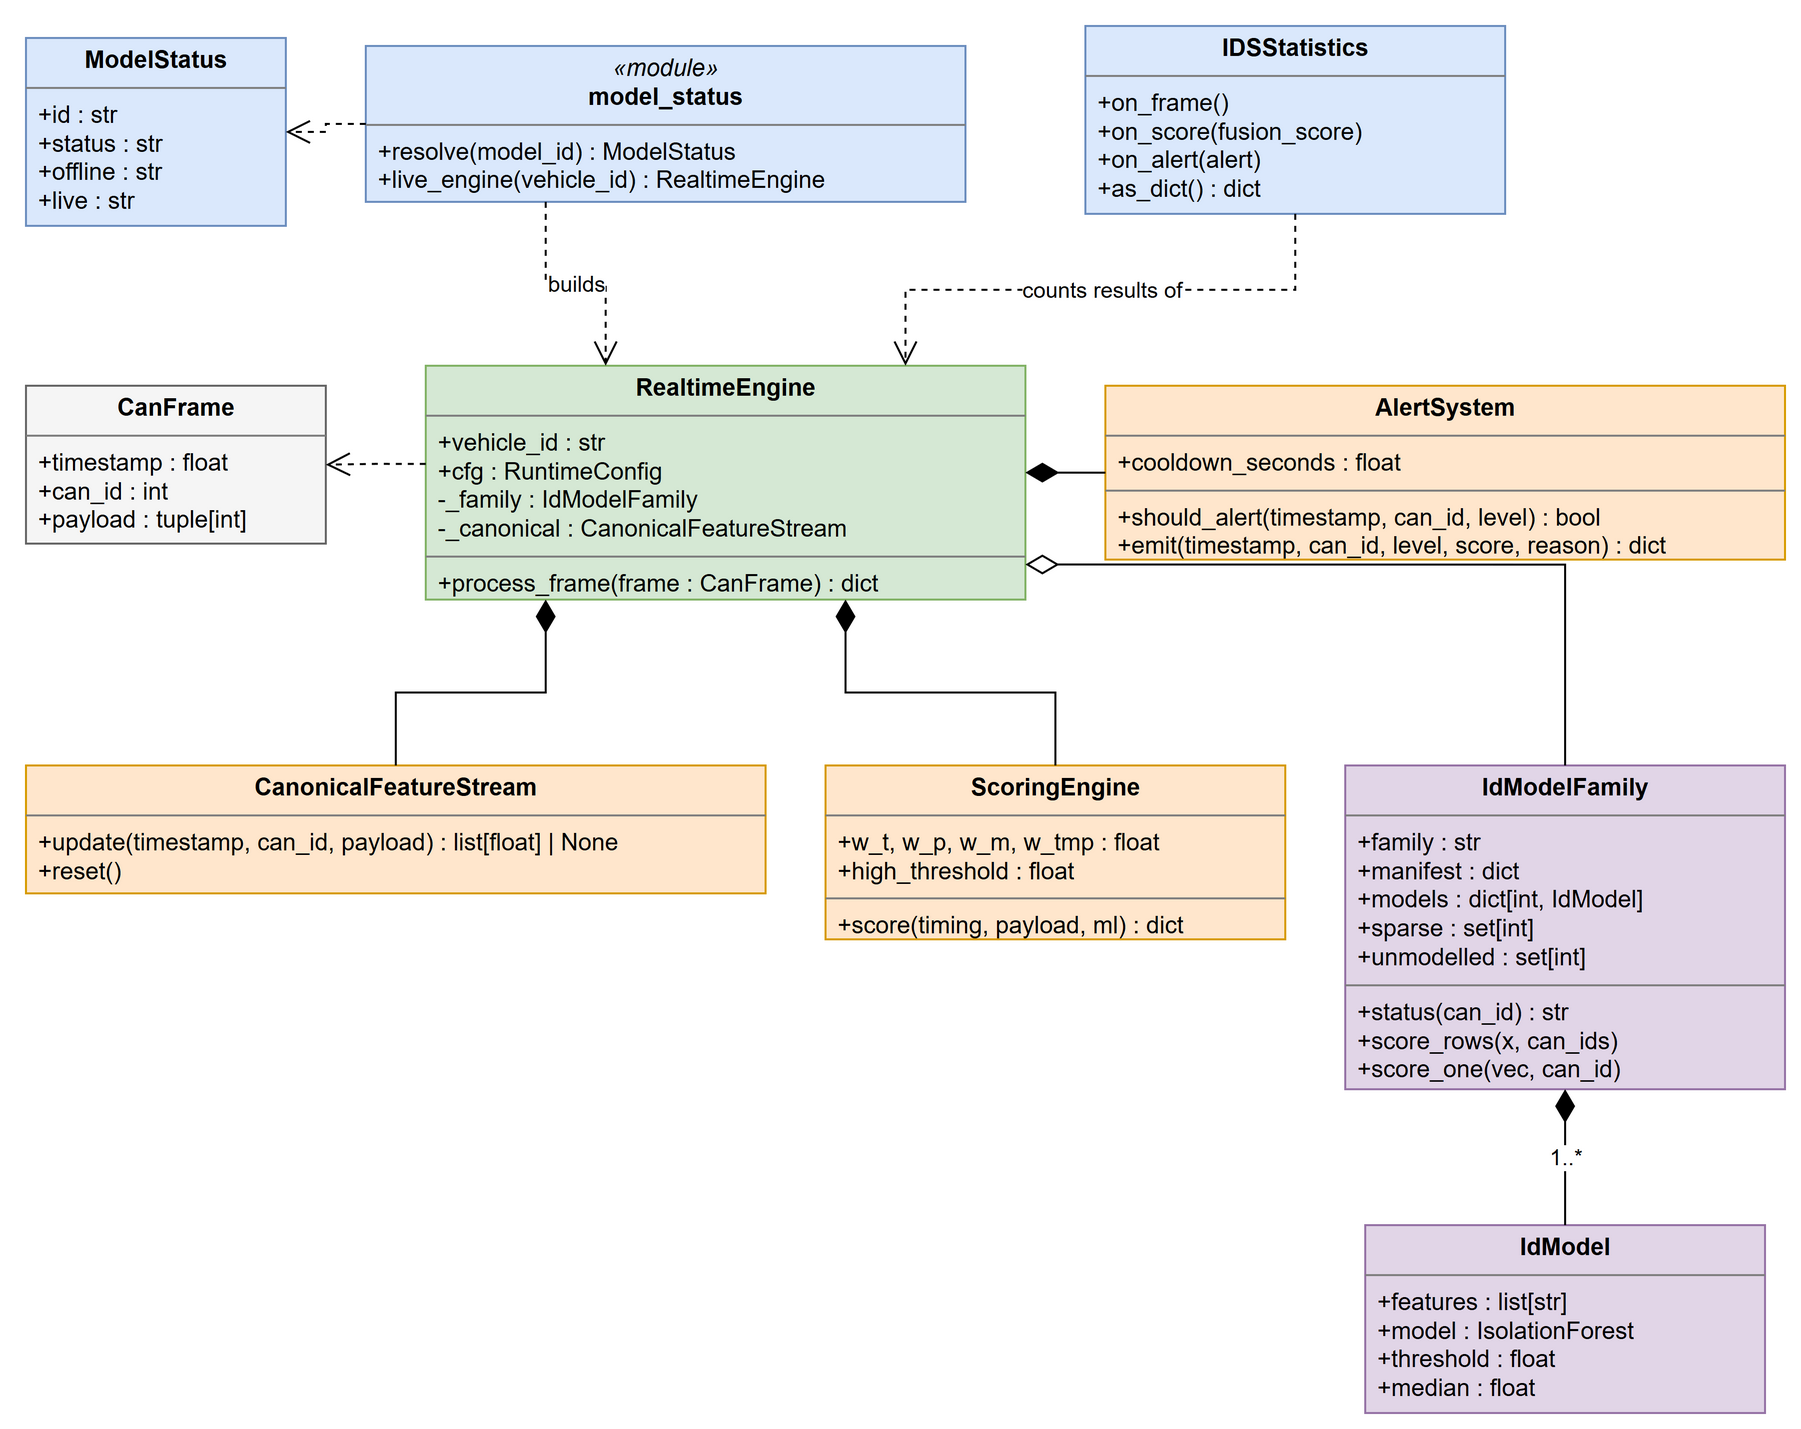
\includegraphics[width=\textwidth]{class_detection_core.png}
\caption{Simplified class diagram of the detection core of the backend.}
\label{fig:class-diagram}
\end{figure}

Figure~\ref{fig:class-client} details the classes of the client. Every screen ViewModel derives from SectionViewModel, which gives it the shared snapshot of the vehicle and access to VehicleDataService. This service owns the state of the session, the alert history and the global state of the application (AppState), and raises events that the screens follow. It calls the backend through PythonApiClient, and CanLogImportService parses a log before an analysis. ModelSelectionService holds the vehicle model chosen by the analyst, and PdfReportBuilder writes the PDF report from the alert list.

\begin{figure}[H]
\centering
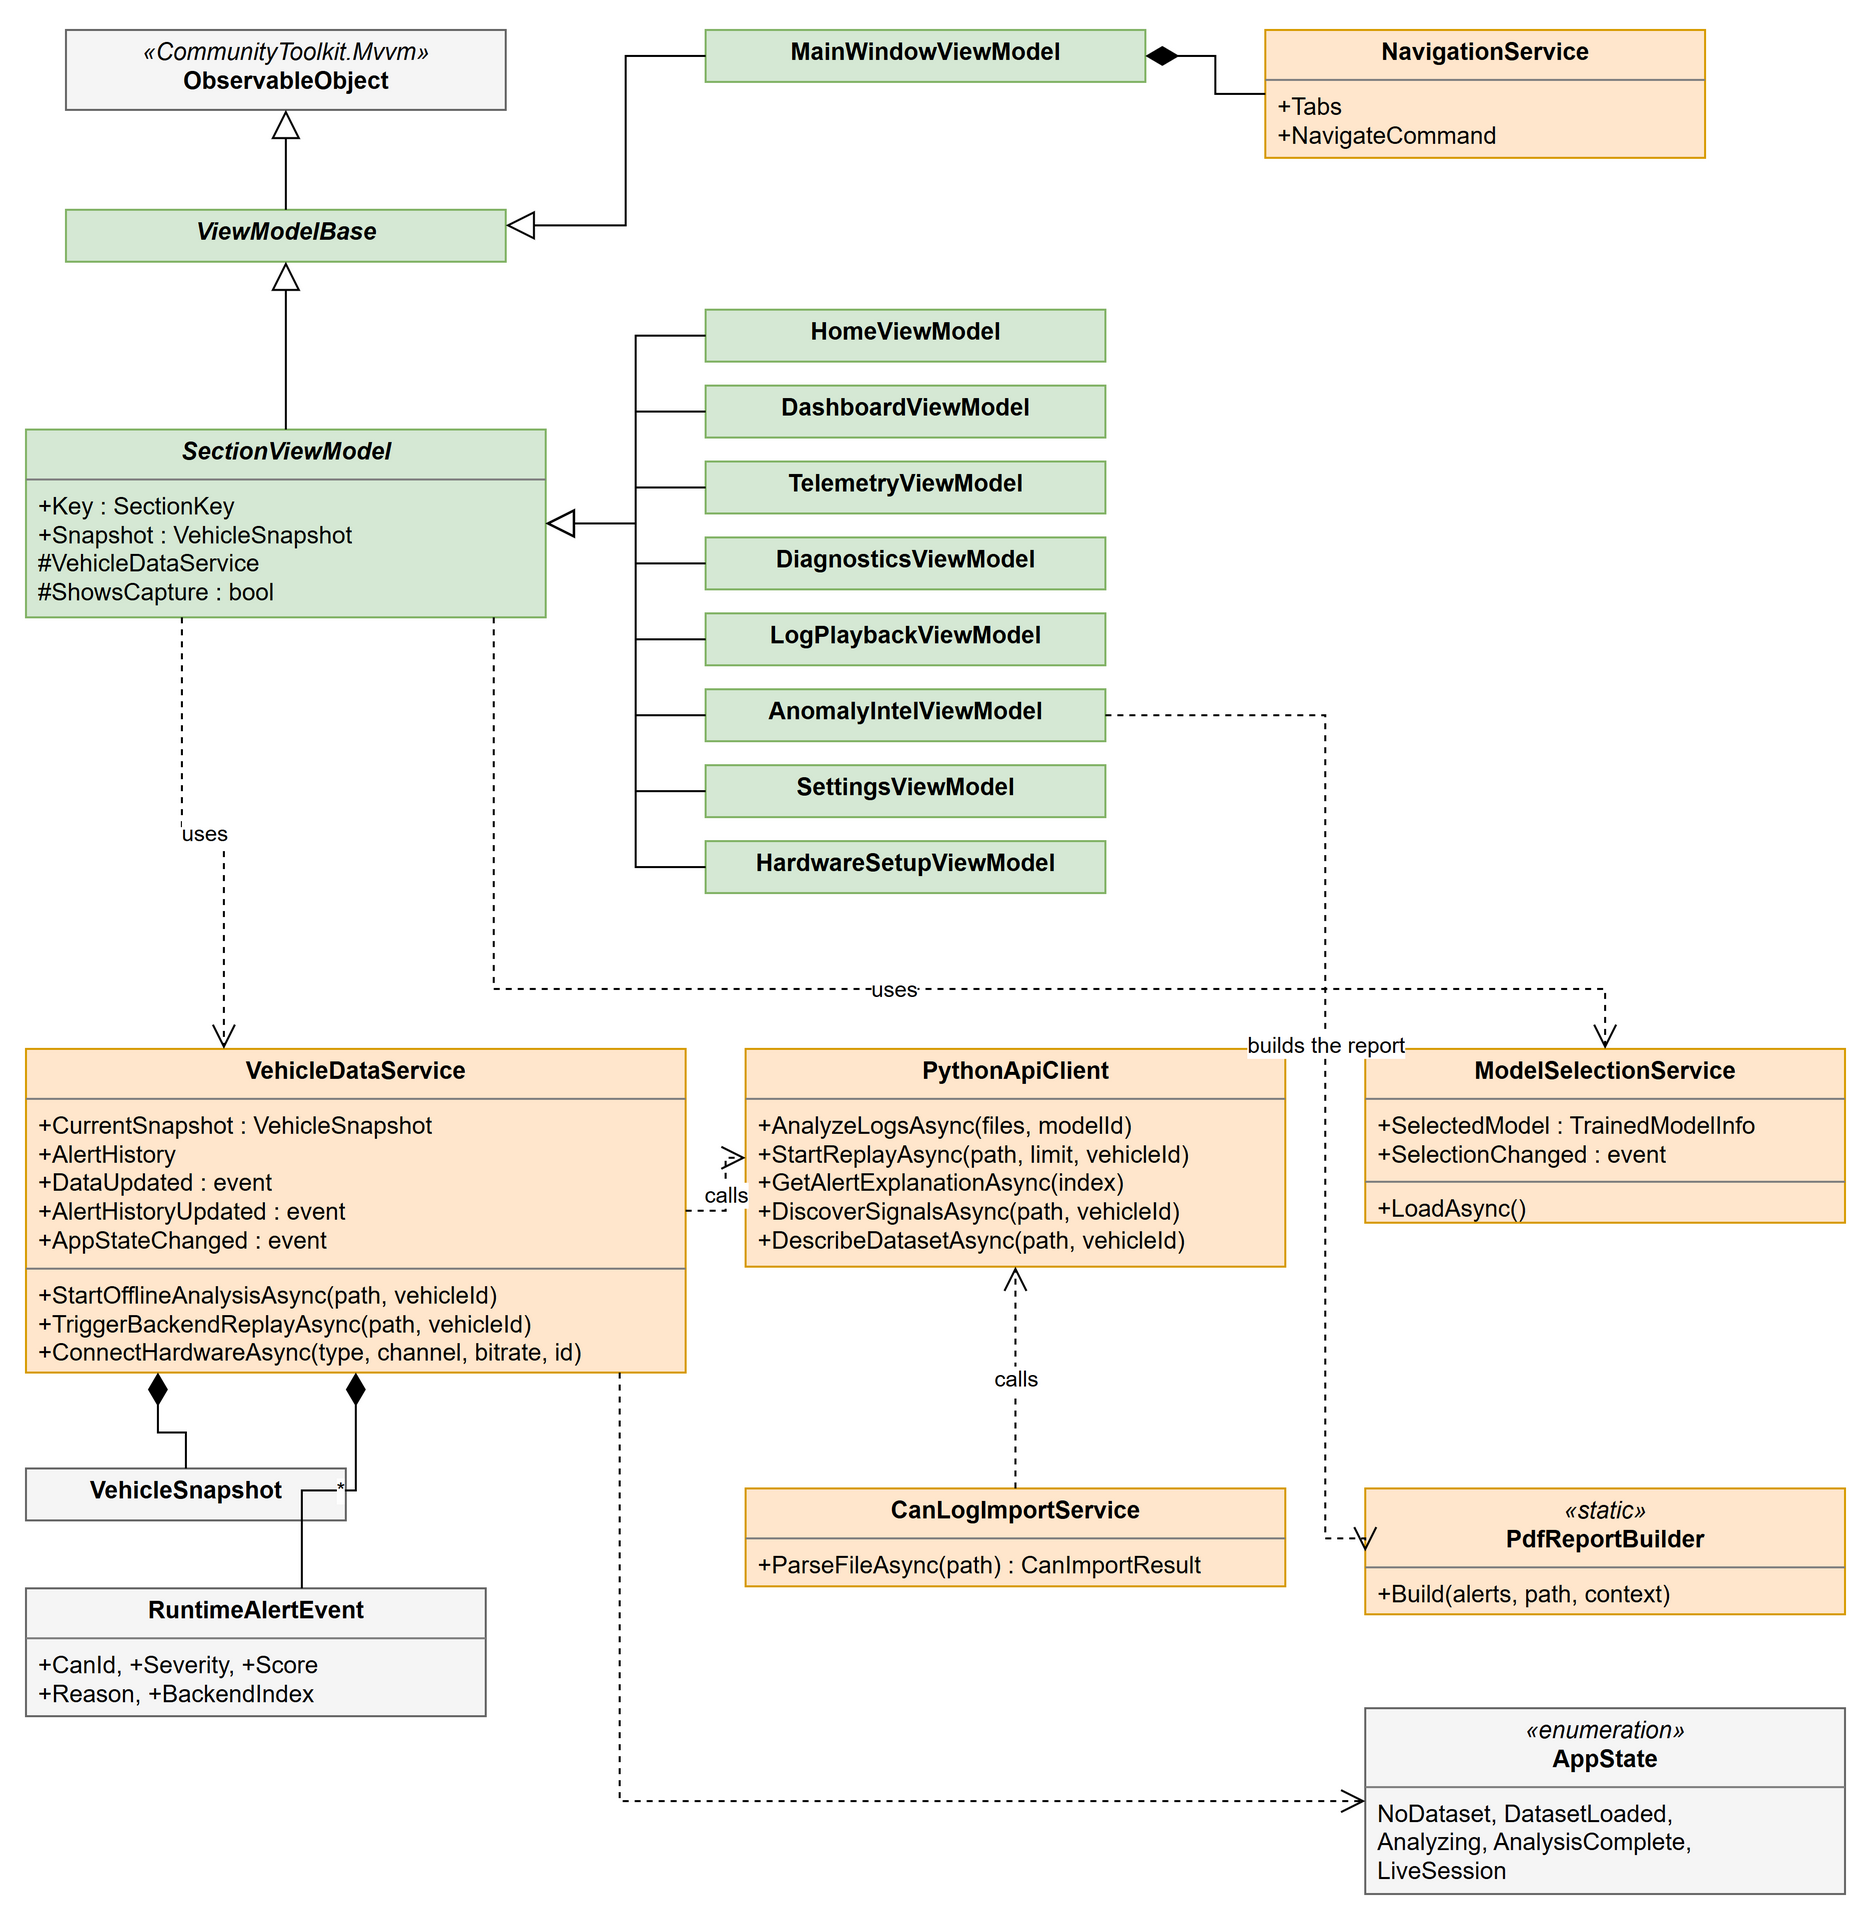
\includegraphics[width=\textwidth]{class_client.png}
\caption{Class diagram of the desktop client.}
\label{fig:class-client}
\end{figure}

\Needspace{464pt}% keep the heading with its float
\subsection{Data model}
\label{sec:data-model}

The backend keeps a small SQLite database (Figure~\ref{fig:data-model}) so that past sessions can be reviewed from a local file. The \code{sessions} table records each session and its source; \code{live\_frames} stores the frames of a session with the result of the detection and an optional label; \code{alert\_history} stores the alerts with their severity, score, reason, temporal pattern and recommended response. The vehicle models are not stored in the database but in model folders, each with its manifest.

\begin{figure}[H]
\centering
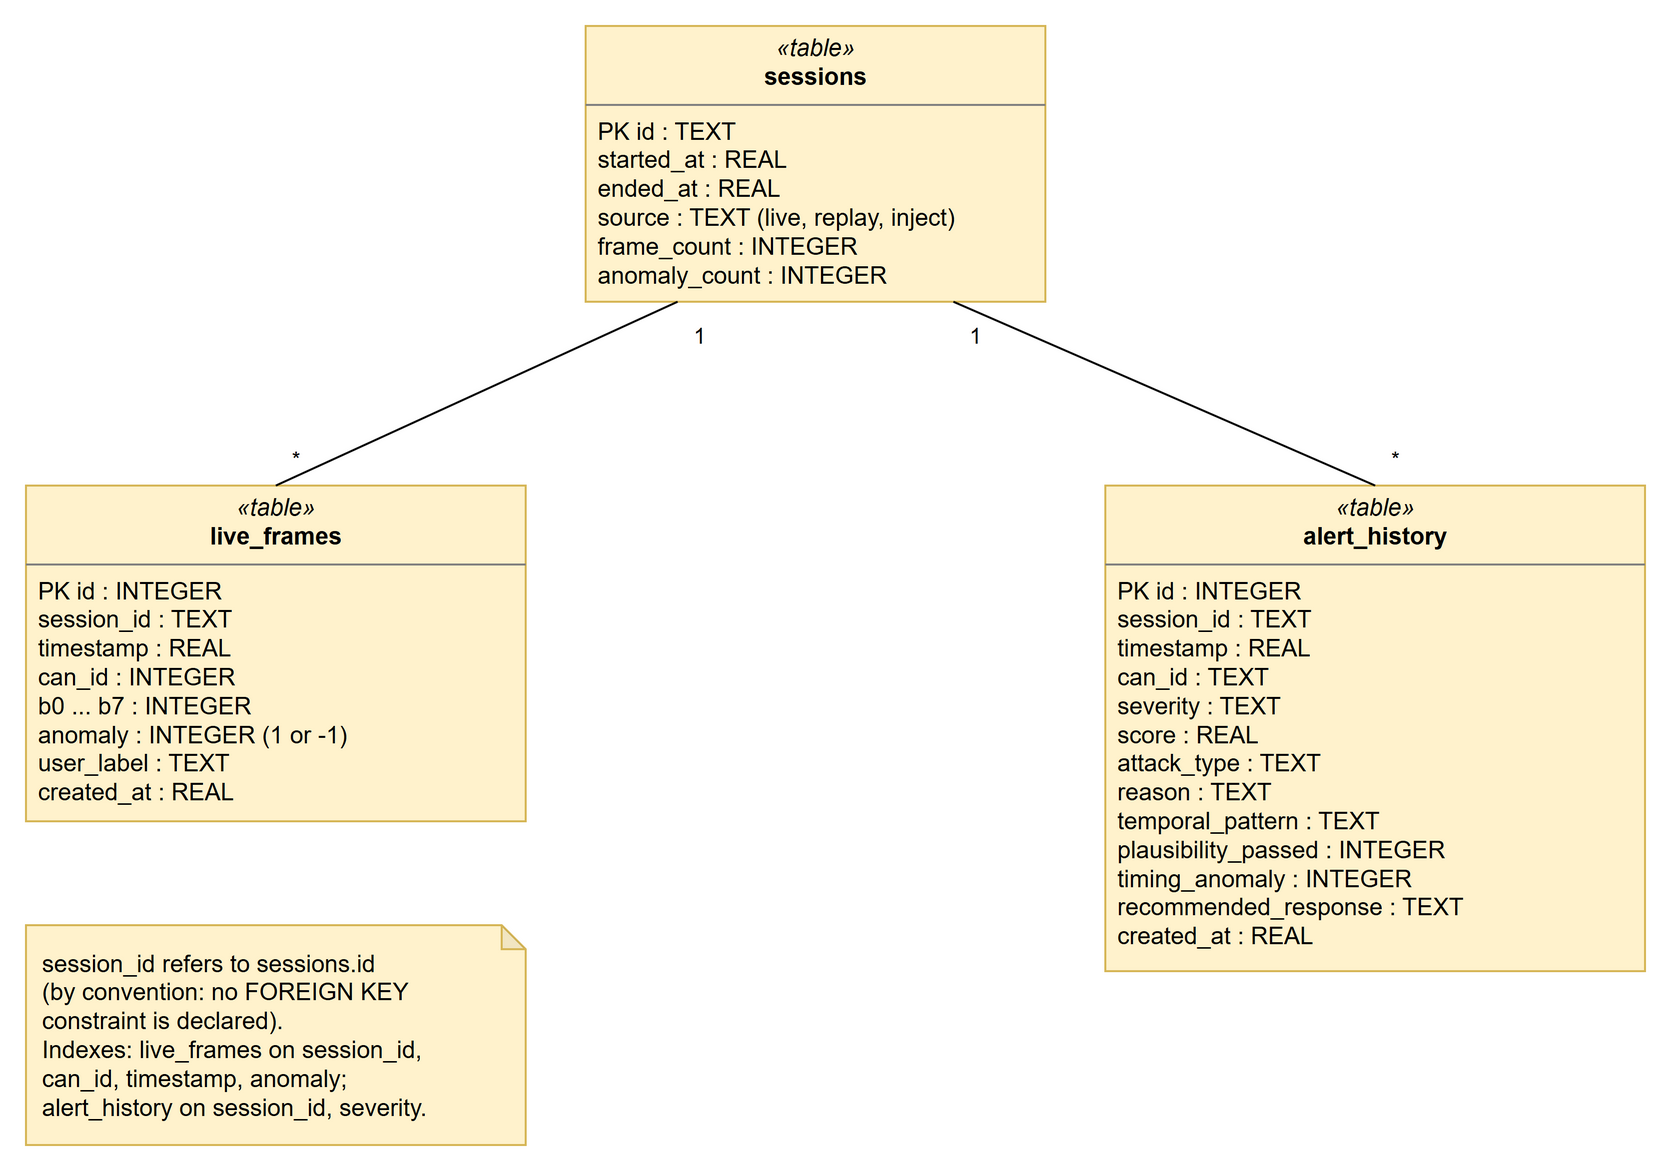
\includegraphics[width=0.9\textwidth]{data_model.png}
\caption{Data model of the SQLite store.}
\label{fig:data-model}
\end{figure}

\section{Dynamic view}

The two sequence diagrams of this section show the key scenarios of a replay and of an explanation. Each object is marked with its nature: \emph{boundary} for the screen the analyst uses, \emph{control} for the objects that coordinate the scenario, and \emph{entity} for the stored data. The messages are numbered in the order in which they are sent; a synchronous call has a filled arrowhead, an asynchronous message an open arrowhead, and a reply a dashed line.

\Needspace{650pt}% keep the heading with its float
\subsection{Life cycle of a replay}
\label{sec:design-replay}

A replay runs in a separate process, so that a long file does not block the backend. It reads the file with the same loader as the offline analysis, so that every format becomes the same stream of (timestamp, identifier, payload) frames, and sends each frame to the same runtime engine as the live and simulated paths. The client follows its progress by polling, and the alerts of the replay are published when it ends so that they can be explained. Figure~\ref{fig:seq-replay} shows this life cycle.

\begin{figure}[H]
\centering
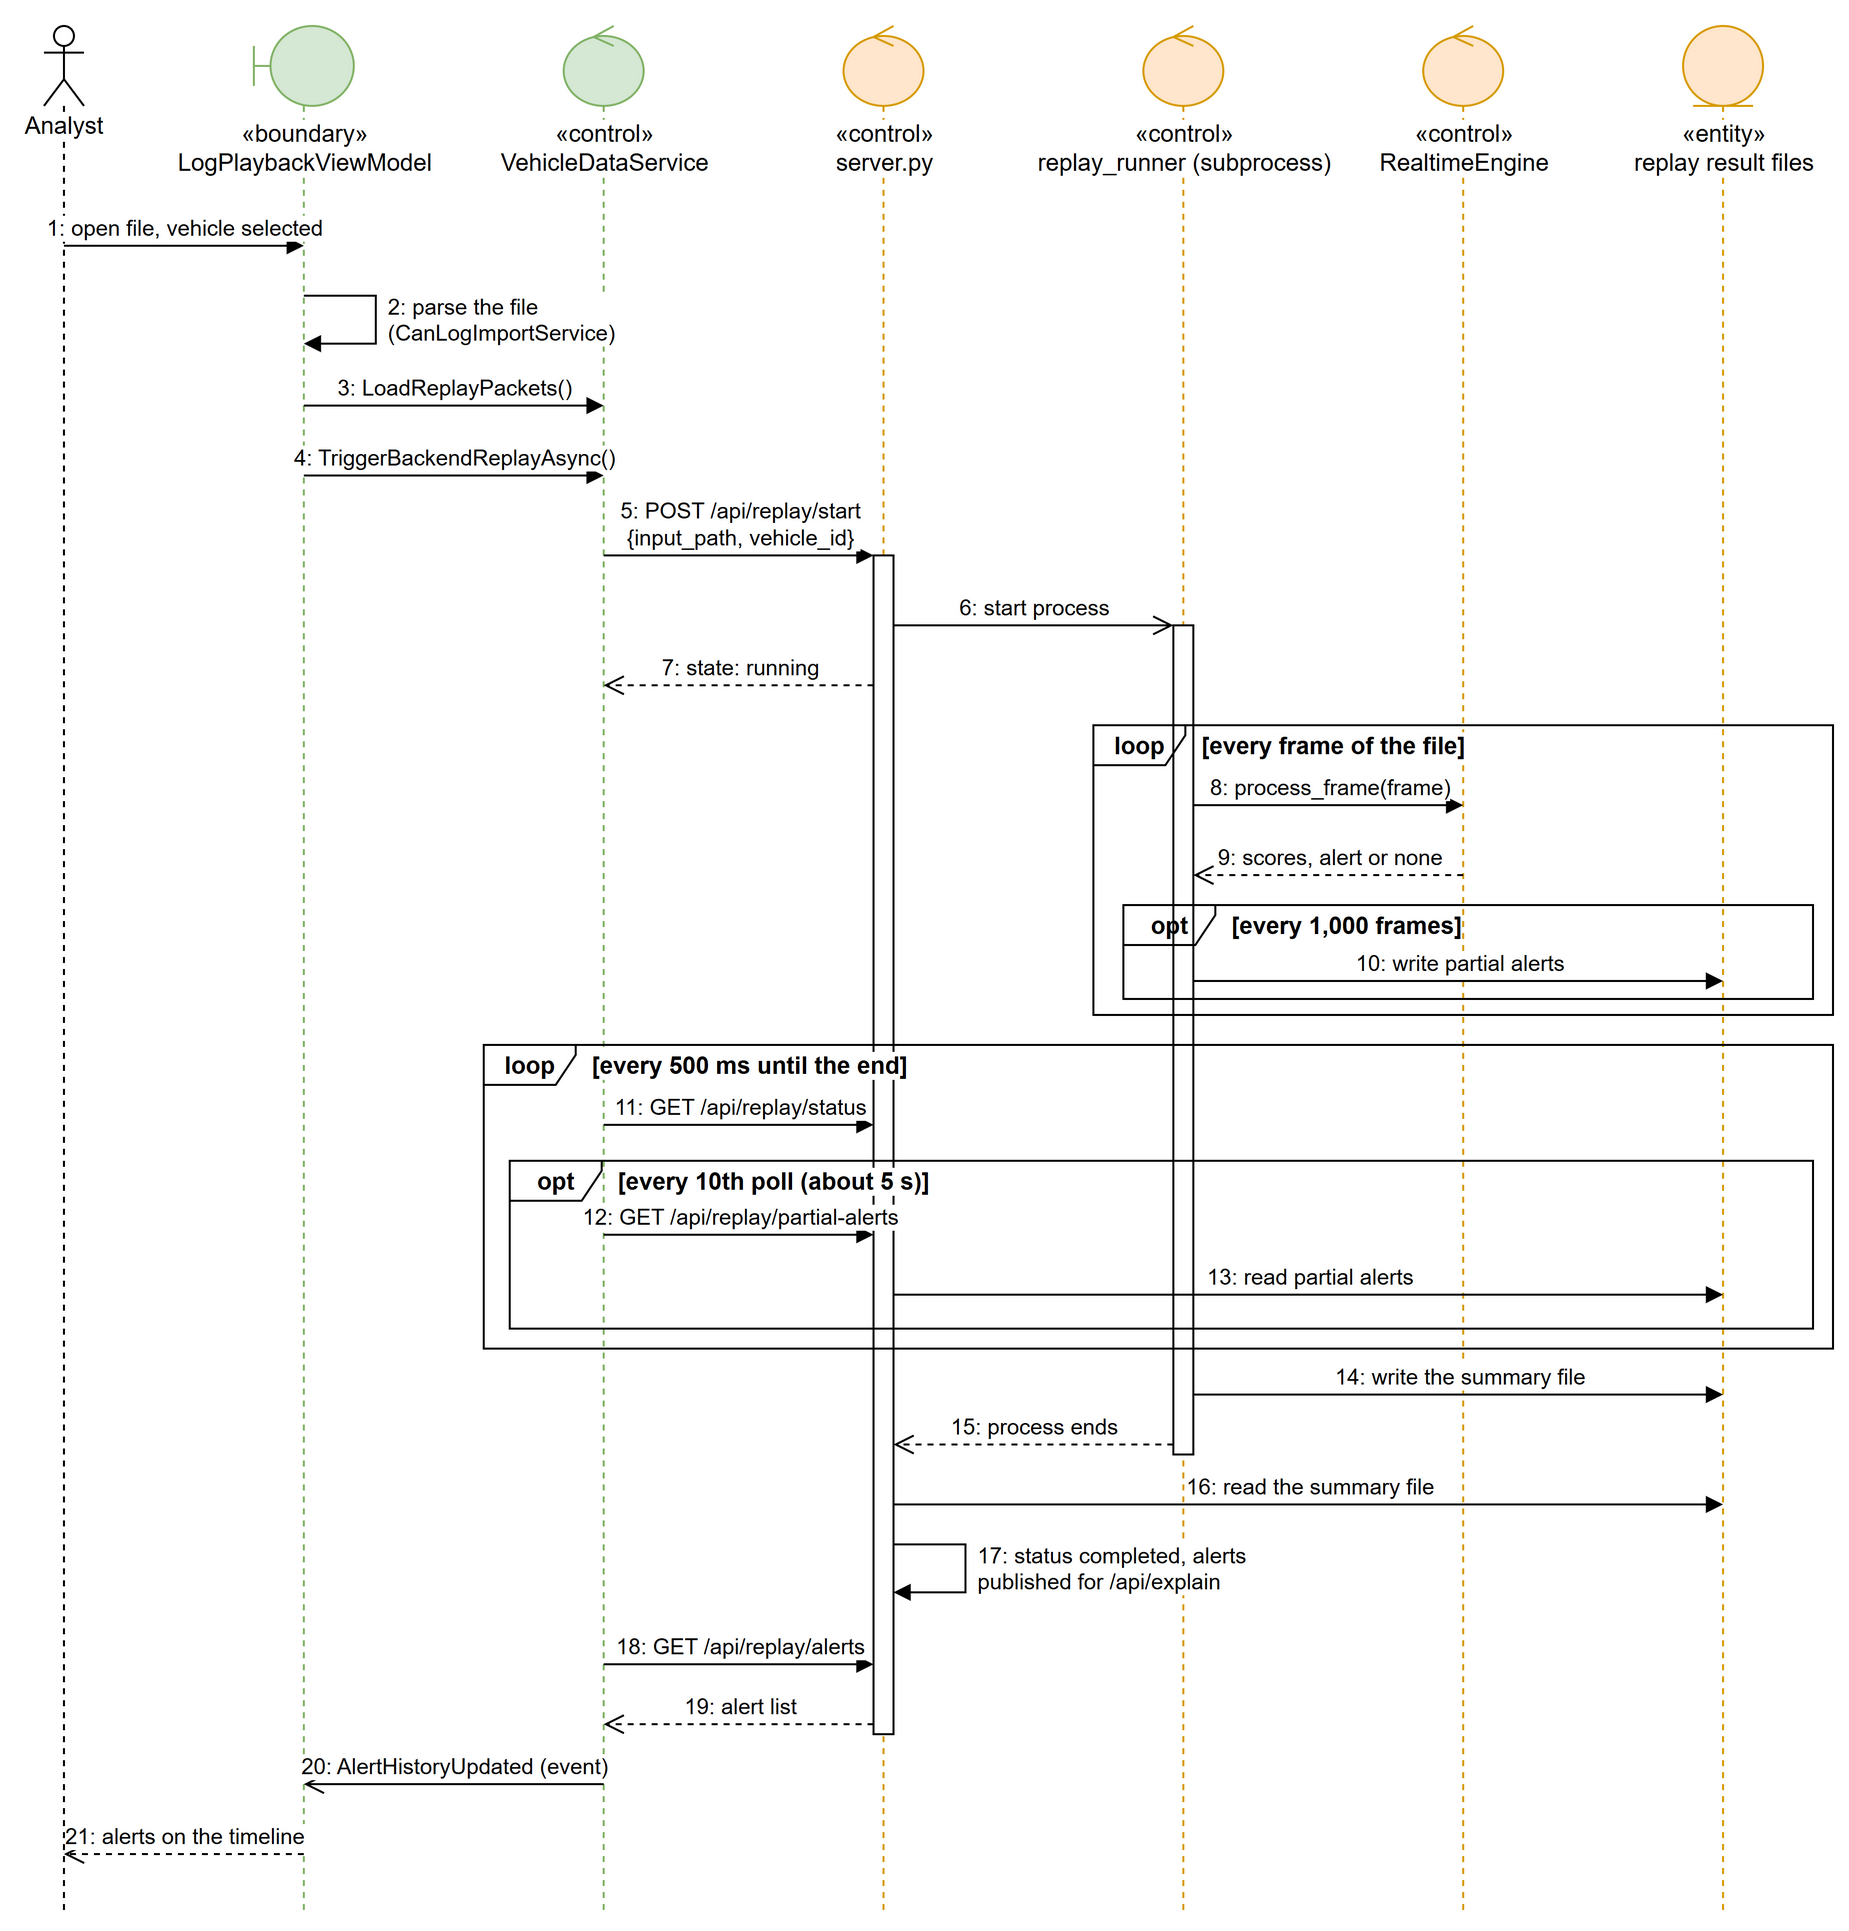
\includegraphics[width=\textwidth]{sequence_replay.png}
\caption[Sequence diagram: life cycle of a replay.]{Sequence diagram: life cycle of a replay, from the client request to the published alerts.}
\label{fig:seq-replay}
\end{figure}

\subsection{Explanation of an alert}
\label{sec:design-ai}

The explanation engine is a supporting feature, not part of detection. It turns the context of an alert into a text an analyst can read: which signal dominated, the likely cause, and what to check. It is called after an alert is raised and never changes a score, a flag or a severity.

When the analyst selects an alert (Figure~\ref{fig:seq-explain}), the backend gathers its context: the measured values and layer scores, the usual behaviour of the identifier, the decoded signals when a \gls{dbc} file exists, known anomaly patterns, similar past cases and, for Gemini, a short web search. Gemini writes the explanation, or a local Ollama model if Gemini cannot be reached; if neither answers, a rule based template fills the same fields from the measured values (NFR6). The engine records the numbers of a model's answer that do not appear in its context, and every answer carries the name of the engine that wrote it, so that a template is never presented as the work of a language model.

\begin{figure}[H]
\centering
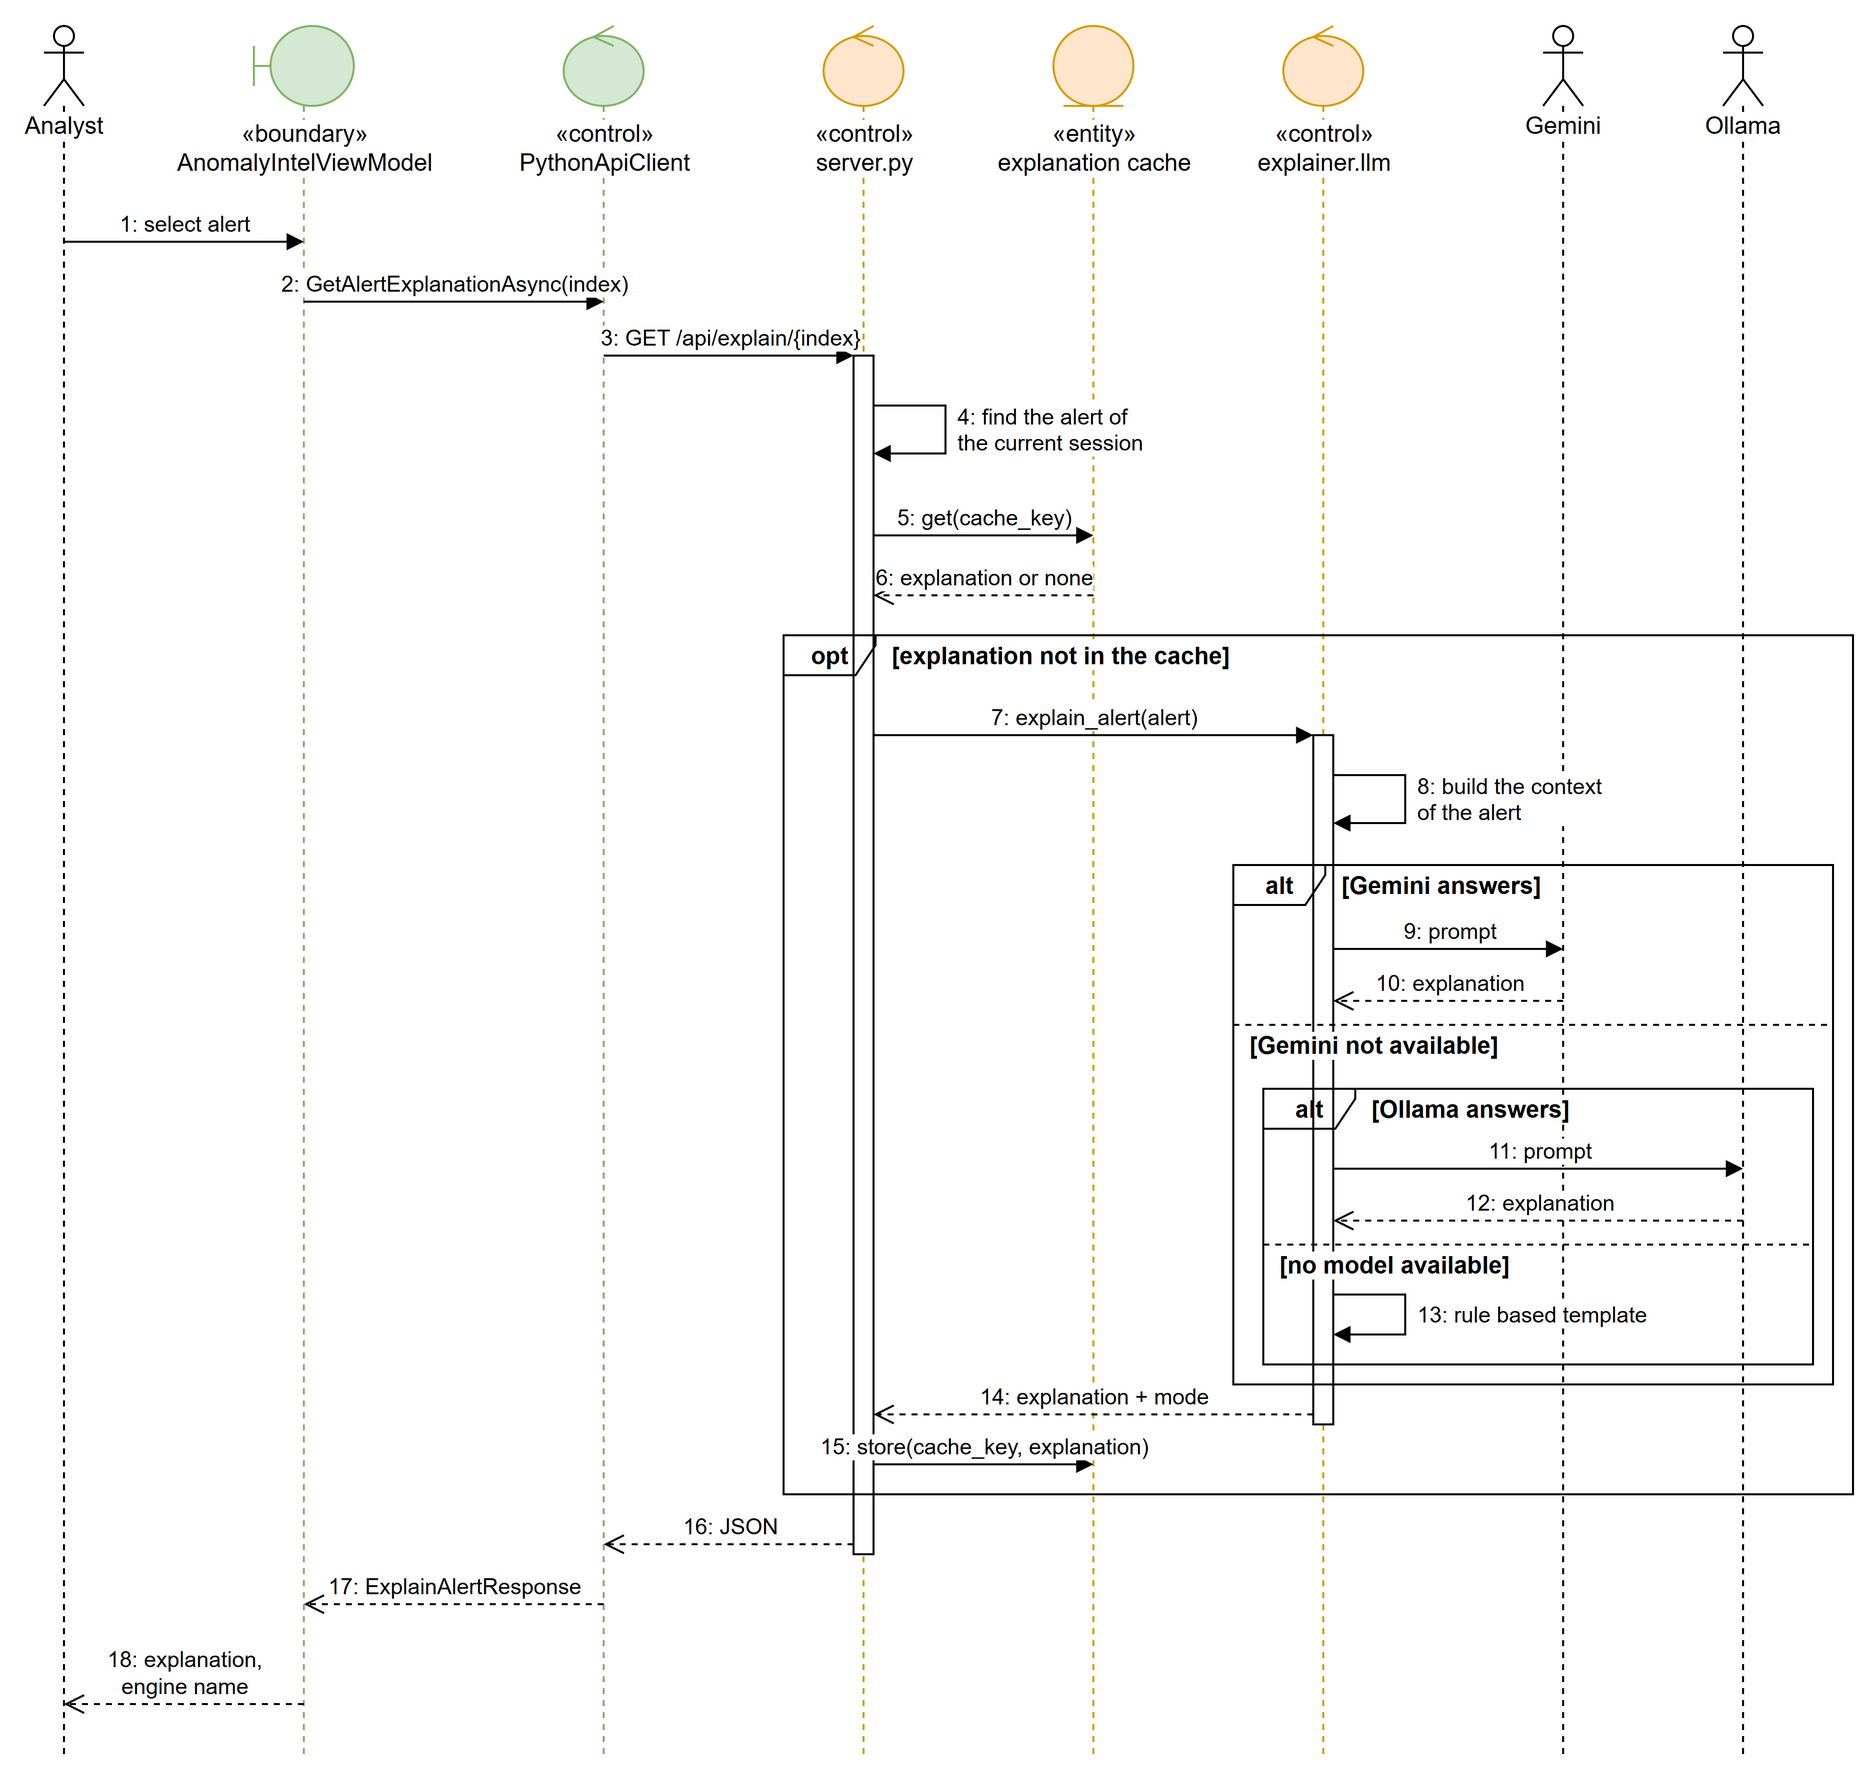
\includegraphics[width=\textwidth]{sequence_explain.png}
\caption{Sequence diagram: requesting the explanation of an alert.}
\label{fig:seq-explain}
\end{figure}

\section{Detection architecture}
\label{sec:design-pipeline}

Frames reach the detection through two paths (Figure~\ref{fig:pipeline}). Replay, simulation and live capture process frames one by one in the runtime engine; the offline analysis receives a whole recording at once. Both use the same features and models, but they turn scores into alerts differently, so the same recording can give different numbers of alerts on each path, and a comparison is only meaningful on one path.

\begin{figure}[H]
\centering
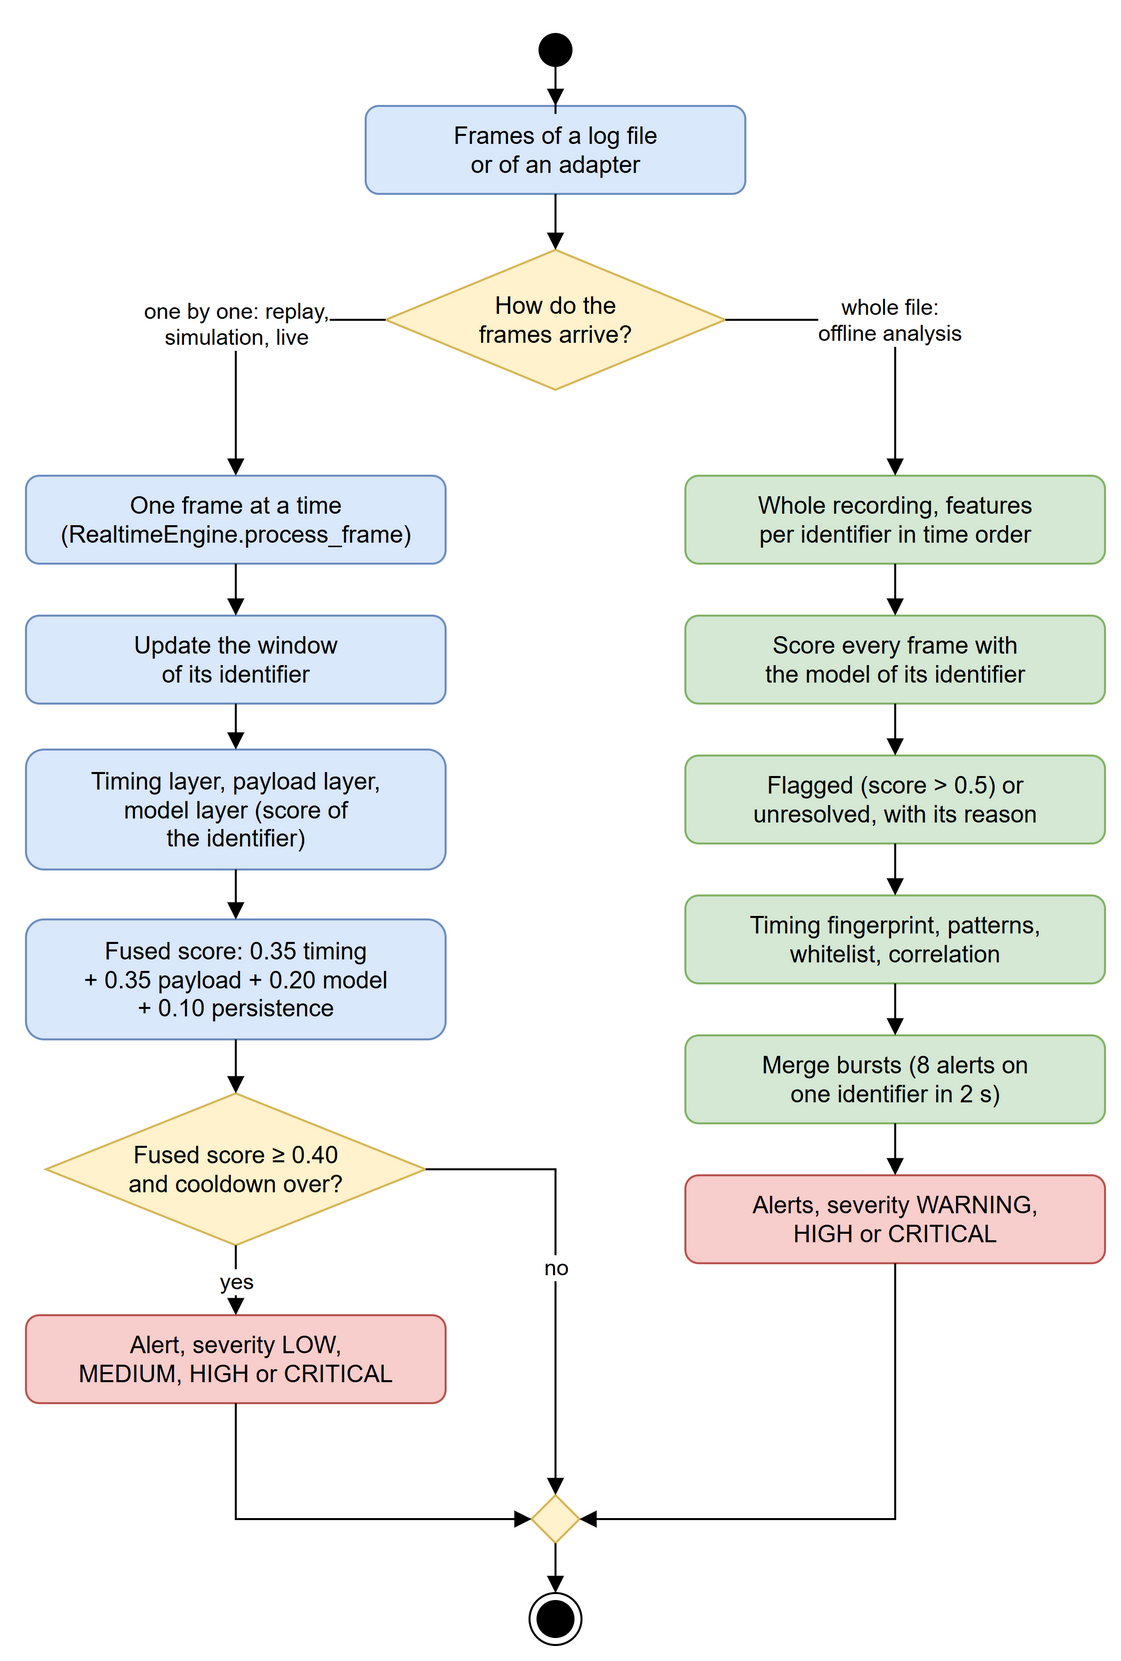
\includegraphics[height=0.66\textheight]{detection_pipeline.png}
\caption[Detection pipeline of the backend.]{Detection pipeline: feature computation per identifier, scoring by the model, additional checks and alerting.}
\label{fig:pipeline}
\end{figure}

\subsection{Frame by frame path (live, simulation, replay)}

For each frame, the runtime engine computes four layer scores:

\begin{itemize}
    \item \textbf{Timing:} The variation of the time between messages of the identifier and its message frequency, whichever is larger, since a regular flood has almost no variation but a very high rate.
    \item \textbf{Payload:} How abruptly the bytes change from one frame of the identifier to the next.
    \item \textbf{Model:} The normalised score given by the model of the vehicle. A frame that no model can score gets no score here, and its status is reported.
    \item \textbf{Persistence:} How many recent frames had a high combined score, so that a sustained anomaly weighs more than a spike.
\end{itemize}

These are combined into one fused score with fixed weights, and Table~\ref{tab:two-paths} gives the alert and severity rules. The weights and thresholds are configuration values, not learned from data.

\begin{table}[H]
\centering
\small
\caption{Scoring and alerting rules of the two detection paths.}
\label{tab:two-paths}
\begin{tabularx}{\textwidth}{|P{2.4cm}|Y|Y|}
\hline
 & \textbf{Frame by frame path (replay, simulation, live)} & \textbf{Offline analysis} \\
\hline
Score & Fused score, each layer from 0 to 2: 0.35 timing + 0.35 payload + 0.20 model + 0.10 persistence & Normalised score of the model, from 0 to 1 \\
\hline
Model call & Every fifth frame of each identifier, the last score reused in between & Every frame \\
\hline
Alert & Fused score $\geq$ 0.40, at most one alert per identifier and second & Each flagged frame (score $>$ 0.5), annotated by the four checks; more than eight alerts on one identifier within two seconds are merged \\
\hline
Severity & LOW $\geq$ 0.30, MEDIUM $\geq$ 0.55, HIGH $\geq$ 0.80, CRITICAL $\geq$ 1.00 & WARNING below 0.55, HIGH $\geq$ 0.55, CRITICAL $\geq$ 0.80; shown in the client as INFO, WARNING and CRITICAL \\
\hline
\end{tabularx}
\end{table}

\subsection{Offline analysis path}

The offline analysis scores every frame with the model of the vehicle. A frame is \emph{flagged} when its score passes the threshold of the model, and a frame that no model can score is counted as \emph{unresolved}, with its reason, instead of normal. Four checks follow: a timing fingerprint of each identifier built from the start of the recording, a frequency analysis that names bursts, frozen payloads and rate spikes, a whitelist of the identifiers seen at the start, and a correlation check between signals linked by a rule, for example a high motor speed with the throttle at zero. Bursts of alerts on one identifier are merged into one summary alert.

\section{Data and machine learning problem framing}
\label{sec:ml-approach}

\subsection{Problem definition}

The learning problem is to decide whether a frame looks like the normal traffic of a given vehicle, without labelled attacks for it. A frame is judged within its own context: a battery voltage message is compared with the usual behaviour of that message, not with the traffic as a whole.

\subsection{Dataset files}
\label{sec:datasets}

All the recordings come from public sources (Figure~\ref{fig:data-logos} and Table~\ref{tab:datasets}); none was bought or obtained under a non disclosure agreement. Only Car-Hacking and the separate attack captures of ROAD carry attack labels.

\begin{figure}[H]
\centering

\includegraphics[height=0.95cm]{css_electronics.pdf}\hspace{0.9cm}

\includegraphics[height=0.95cm]{ornl.pdf}\hspace{0.9cm}

\includegraphics[height=0.95cm]{korea_university.pdf}\hspace{0.9cm}

\includegraphics[height=0.95cm]{github.pdf}
\caption[Sources of the recordings.]{Sources of the recordings: CSS Electronics, Oak Ridge National Laboratory (ROAD), Korea University (Car-Hacking) and GitHub (EV-CANlogs).}
\label{fig:data-logos}
\end{figure}

\begin{table}[H]
\centering
\small
\caption{Dataset files used in the project.}
\label{tab:datasets}
\begin{tabularx}{\textwidth}{|P{2.7cm}|P{3.1cm}|P{2.0cm}|Y|}
\hline
\textbf{Dataset} & \textbf{Vehicles} & \textbf{Format} & \textbf{Use in the project} \\
\hline
CSS Electronics sample data, including the EV Data Pack~\cite{css_evdata} & Kia EV6, Nissan Leaf 2019 & \gls{mf4} & Kia EV6: validation of the first pipeline; Nissan Leaf 2019: training and holdout of a final model \\
\hline
ROAD~\cite{verma2020road} & Real vehicle on a dynamometer & candump log & Ambient recordings only: first corpus, training and holdout of the ROAD ambient model \\
\hline
Car-Hacking~\cite{seo2018gids} & Real vehicle & \gls{csv} with labels & Normal rows only, in the first corpus \\
\hline
EV-CANlogs~\cite{evcanlogs} & Jaguar I-PACE, Kia EV6, BMW i3, MG ZS EV, Tesla and others & \gls{csv}, candump, Vector & Most of the first corpus; training and holdout of the Jaguar I-PACE and Kia EV6 models \\
\hline
Renault Clio log & Renault Clio & candump log & Only to check that no data leaks between sessions \\
\hline
\end{tabularx}
\end{table}

\subsection{Supervised or unsupervised learning}

A supervised approach would need labelled normal and attack frames for every vehicle. Most of the corpus has no labels, the few labelled attacks come from other vehicles and attack methods, a model trained on known attacks is unlikely to recognise a new one, and recording real attacks on every vehicle was not possible. An unsupervised approach only needs the normal traffic of the vehicle, which the corpus has in plenty.

\subsection{Candidate algorithms}
\label{sec:ml-selection}

Table~\ref{tab:ml-comparison} compares the algorithms considered for the anomaly score.

\begin{table}[H]
\centering
\footnotesize
\caption{Candidate machine learning algorithms for the anomaly score.}
\label{tab:ml-comparison}
\begin{tabularx}{\textwidth}{|P{3.1cm}|Y|P{2.6cm}|}
\hline
\textbf{Algorithm} & \textbf{Advantages} & \textbf{Disadvantages} \\
\hline
Isolation Forest~\cite{liu2008isolation} & Fast to train, no distance computation, no assumption on the distribution; suited to numeric tabular features. & Harder to read than a rule; needs a decision threshold. \\
\hline
One Class SVM~\cite{scholkopf2001estimating} & Well studied, with a clear geometric meaning. & Training cost grows fast with the data; sensitive to its kernel. \\
\hline
Local Outlier Factor (LOF)~\cite{breunig2000lof} & Captures local differences of density. & Keeps the training data; its prediction cost grows with it. \\
\hline
DBSCAN~\cite{ester1996density} & Finds clusters of any shape without fixing their number. & Gives no score for a new point. \\
\hline
Random Forest (supervised) & Very accurate with labelled data. & Needs labelled attacks for each vehicle. \\
\hline
Autoencoder & Can model complex normal patterns. & Needs more data and tuning; harder to explain. \\
\hline
K-Means~\cite{macqueen1967methods} & Simple and fast. & Not an anomaly detector by itself. \\
\hline
\end{tabularx}
\normalsize
\end{table}

\subsection{Choice of Isolation Forest}

The algorithm had to learn from normal data only, give a result an analyst can understand (``how unusual is this frame''), and score a frame quickly enough for replay and live capture. Isolation Forest meets the first two criteria by construction: it is trained on normal traffic, and an anomalous point is isolated after fewer random splits. DBSCAN was set aside because it gives no score for a new frame, the autoencoder because it is harder to explain and debug, and the supervised Random Forest because no labelled attacks exist for our vehicles. LOF and the One Class SVM remained credible alternatives, so we planned to measure them against Isolation Forest once the final models existed, on the same data and under the same rule.

\section{Architecture baseline}
\label{sec:baseline}

The elaboration phase ended with an executable architecture, delivered by milestone M1, the live foundation. It connected the two programs end to end before any vehicle model existed: the client started and stopped a live session through new \gls{api} endpoints, the backend scored a simulated stream frame by frame in the runtime engine, an alert reached the client, and the Dashboard charted the fused score of the last frames. A smoke test checked this chain, from the simulated data to the scoring, the alert and the update of the Dashboard.

This baseline reduced three risks of Table~\ref{tab:risks}. Live capture would only differ from replay and simulation by its transport, since all three feed the same runtime engine (R1). Every source would enter the engine as the same frame representation (R7). And the client and the backend were shown to work together through the \gls{api}, so that the following iterations could add features on both sides without changing how they communicate.

\section{Conclusion}

This chapter presented the technical choices, the architecture of the client and the backend, the domain and data models, the dynamic view of a replay and of an explanation, the two detection paths, the framing of the machine learning problem, and the architecture baseline of the elaboration phase. The next chapter presents the four iterations of the construction phase.

\chapter{Construction: Iterations}
\label{chap:construction}

\section*{Introduction}
\addcontentsline{toc}{section}{Introduction}

This chapter presents the construction phase, during which CANvisionNative was built on the architecture baseline of Chapter~\ref{chap:elaboration}. It first explains how the work of the phase was planned in iterations, then presents the four iterations one after the other: the first detection pipeline and client, its validation and correction on a real recording, the hardware layer and its bench rig, and the rebuild of the vehicle models.

\section{Iteration planning}
\label{sec:it-planning}

The construction phase was divided into four iterations, each one addressing some of the risks of Table~\ref{tab:risks}. Each iteration is presented with the same template: its objectives, the use cases it addressed, its design, its implementation, its tests, and an assessment that decided what the next iteration had to do. Table~\ref{tab:iterations} gives the period, the goal and the main risks addressed by each iteration.

\begin{table}[H]
\centering
\small
\caption{Iterations of the construction phase.}
\label{tab:iterations}
\begin{tabularx}{\textwidth}{|P{1.8cm}|P{2.2cm}|Y|P{3.4cm}|}
\hline
\textbf{Iteration} & \textbf{Period (2026)} & \textbf{Goal} & \textbf{Main risks addressed} \\
\hline
1 & March to June & First detection pipeline and client (M3 to M8) & R2, R7 \\
\hline
2 & June to July & Validation and correction on a Kia EV6 recording & R3, R6, R7, R8 \\
\hline
3 & August to September & Hardware layer and bench rig (M2) & R1 \\
\hline
4 & September & Model rebuild and evaluation on recordings kept out of training & R3, R4, R5, R6 \\
\hline
\end{tabularx}
\end{table}

% ============================================================
\section{Iteration 1: first detection pipeline and client}
\label{sec:it1}

\subsection{Objectives}

The first iteration delivered milestones M3 to M8 on the architecture baseline: models trained for several vehicles and driving states (M3), the explanation engine (M4), the real time charts (M5), session recording (M6), the integration of the client and the backend (M7), and the decoding pipeline for offline and live traffic (M8). At its end, an analyst could import a log, analyse and replay it, review and explain its alerts, and export them.

\subsection{Use cases addressed}

This iteration addressed the use cases \emph{Import log}, \emph{Select vehicle}, \emph{Replay log}, \emph{Start live simulation}, \emph{Detect anomaly}, \emph{Record session}, \emph{Review alerts}, \emph{Request explanation}, \emph{Export report} and \emph{Configure settings}, which together cover the work of the analyst on a recorded log. The use cases \emph{Connect hardware}, \emph{Check model status} and \emph{Describe capture} were addressed in later iterations.

\subsection{Design: a first model based on driving states}
\label{sec:impl-state}

The first design routed each frame through a driving state. Fourteen rolling features were computed for every identifier, a K-Means model shared by all vehicles classified the state as parking, idle or driving (Figure~\ref{fig:state-vehicle}), and the frame was scored by the Isolation Forest of that state and vehicle. When no forest matched, the engine fell back to a generic model, then to a heuristic. These models were trained on more than seven million frames from sixty six sources of the corpus of Table~\ref{tab:datasets}.

\begin{figure}[H]
\centering
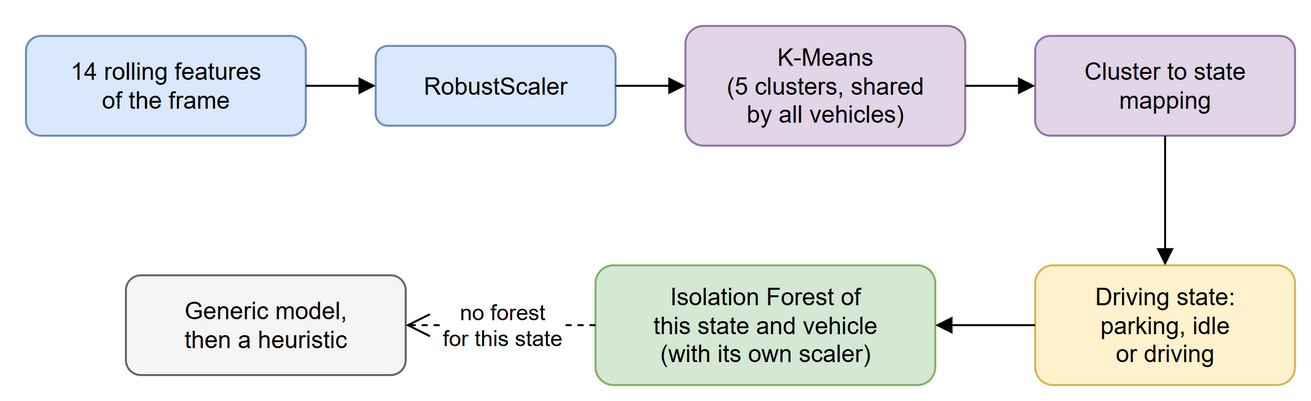
\includegraphics[width=\textwidth]{state_vehicle.png}
\caption[Scoring path of the first design.]{Scoring path of the first design: K-Means on fourteen rolling features chose the driving state, which selected the Isolation Forest.}
\label{fig:state-vehicle}
\end{figure}

\subsection{Implementation}

The iteration implemented the backend services below on the architecture baseline, then the screens and exports of the client.

\subsubsection{Parser and common frame representation}
\label{sec:impl-parser}

One dispatch function turns every supported format into the same stream of (timestamp, identifier, payload) frames:

\begin{itemize}
    \item \textbf{.csv:} Generic columns, or the SavvyCAN columns with timestamps in microseconds.
    \item \textbf{.mf4:} ASAM \gls{mf4}~\cite{asam_mdf} binary logs, read with asammdf.
    \item \textbf{.asc:} The Vector text format.
    \item \textbf{.log:} The candump and SocketCAN format, including its timestamped variant.
    \item \textbf{.txt:} The PCAN text format, with candump parsing as a fallback.
\end{itemize}

The offline analysis called this function from the start. The replay engine, however, still had its own loader, which only understood \gls{csv}; this gap was found and closed in the second iteration (Fix 4).

\subsubsection{Replay engine}
\label{sec:impl-replay}

The replay process writes partial results during the run, so that the client can show progress, and a summary with the full alert list at the end. In the client, the Log Playback screen plays the frames at the pace of their own timestamps, multiplied by the chosen speed; a first version played one frame per screen refresh, which ran a bus of 3{,}000 frames per second about fifty times slower than real time.

\Needspace{335pt}% keep the heading with its float
\subsubsection{Vehicle profiles}
\label{sec:impl-vehicle}

Two registries describe the vehicles. The vehicle profiles (Table~\ref{tab:vehicles}) give a bitrate and the \gls{dbc} files that decode the frames; the last one was written for the bench rig in the third iteration. The second registry lists the trained models of each vehicle. The two lists do not match one to one: the Jaguar I-PACE has a model but no \gls{dbc} file, while the BMW i3 has a \gls{dbc} file but only a model of the first design.

\begin{table}[H]
\centering
\small
\caption{Vehicle profiles with \acrshort{dbc} decoding.}
\label{tab:vehicles}
\begin{tabular}{|l|l|c|}
\hline
\textbf{Identifier} & \textbf{Display name} & \textbf{Bitrate} \\
\hline
nissan\_leaf    & Nissan Leaf (2019, 40/62 kWh) & 500 kbps \\
\hline
hyundai\_ioniq5 & Hyundai Ioniq 5               & 500 kbps \\
\hline
hyundai\_kia    & Hyundai / Kia (generic)       & 500 kbps \\
\hline
skoda\_enyaq    & Škoda Enyaq iV (VW MEB)       & 500 kbps \\
\hline
vw\_skoda\_audi & VW / Škoda / Audi (generic)   & 500 kbps \\
\hline
renault\_zoe    & Renault Zoe                   & 500 kbps \\
\hline
tesla\_model3   & Tesla Model 3                 & 500 kbps \\
\hline
kia\_ev6        & Kia EV6                       & 500 kbps \\
\hline
bmw\_i3         & BMW i3 (2017, 60 Ah REX)      & 500 kbps \\
\hline
bench\_rig      & Arduino bench rig             & 500 kbps \\
\hline
\end{tabular}
\end{table}

\subsubsection{Explanation module}

The explanation module implements the design of \Sref{sec:design-ai}. The context of an alert is built in the backend, and the providers are called in turn through their \gls{http} interfaces. Each explanation is added to a history store, so that later similar anomalies can refer to it, and cached during a run, so that the same alert is not explained twice.

\subsubsection{Client and exports}

The client implements the seven screens of \Sref{sec:design-frontend}, presented in Chapter~\ref{chap:transition}. Anomaly Intel exports the alert list as a \gls{csv} file or as a PDF report built with PDFsharp, both read from the list on screen.

\subsection{Tests}

Each milestone was checked by running it on recorded logs and by a demonstration in the client before the next one started. The systematic validation of the whole pipeline on a real recording was left to the second iteration.

\subsection{Assessment}

All the milestones M3 to M8 were delivered, and the first pipeline worked from the import of a log to the export of its alerts. It had not yet been checked against facts known independently, which was the goal of the second iteration.

% ============================================================
\section{Iteration 2: validation and correction on the Kia EV6}
\label{sec:it2}

\subsection{Objectives}

The second iteration validated the first pipeline on a real recording, found its defects and corrected them. One rule guided it (NFR2): a claim had to be backed by reproducible evidence before any code was changed. Tuning a threshold or retraining blindly were not accepted as fixes. A defect counted as found only once it could be triggered on demand and explained in the code, and as fixed only once the same test, run again, gave the expected result.

\subsection{Use cases addressed}

The validation followed the path of an analyst on a recording, through the use cases \emph{Import log}, \emph{Select vehicle}, \emph{Replay log} and \emph{Detect anomaly}, then \emph{Request explanation} and \emph{Export report} on the alerts that the replay produced.

\Needspace{388pt}% keep the text with its float
\Needspace{374pt}% keep the heading with its float
\subsection{Design of the validation}

The validation took three passes (Figure~\ref{fig:validation-workflow}): an audit of the interface, an analysis of the root causes of the alerts, and the correction of the defects, each verified again, followed by a full run of the corrected pipeline.

\begin{figure}[H]
\centering
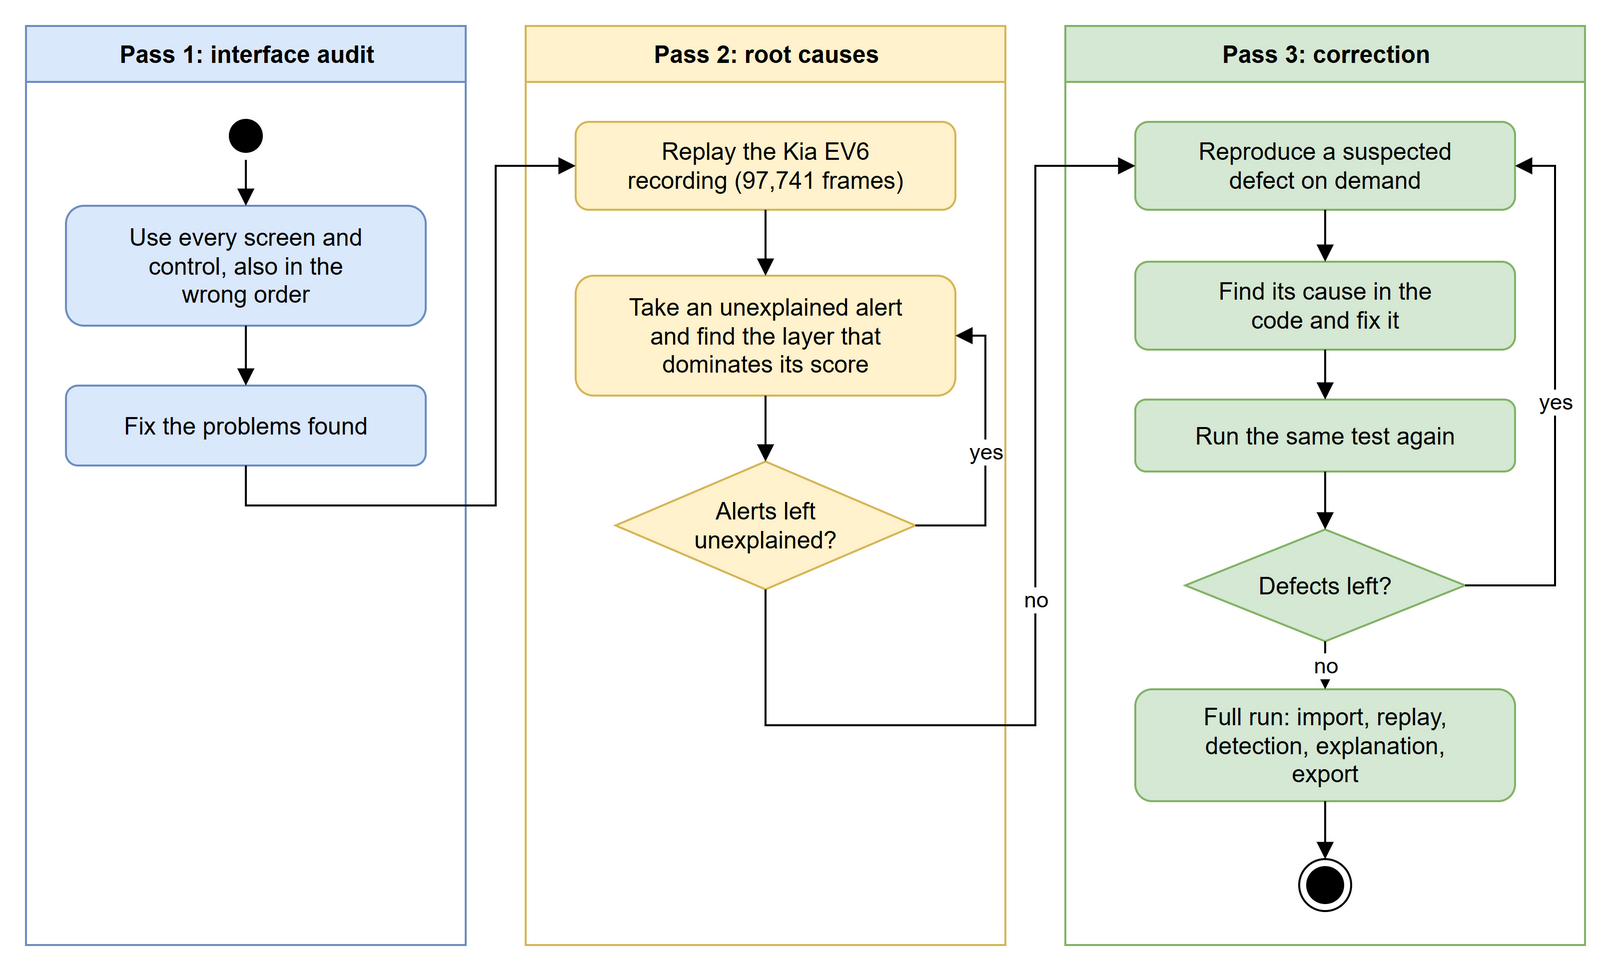
\includegraphics[width=0.9\textwidth]{validation_workflow.png}
\caption{Passes of the validation of the first pipeline.}
\label{fig:validation-workflow}
\end{figure}

\label{sec:validation-setup}
The iteration used a one hour recording of a Kia EV6 (\texttt{00000158-\allowbreak 64CBC290.MF4}) from the CSS Electronics EV Data Pack (Table~\ref{tab:datasets}), captured by a CANedge logger that actively polled the \glspl{ecu} with \gls{uds} requests. After conversion, it contains \textbf{97{,}741 frames}. It was the only available recording that came from an unmodified production vehicle, was long enough for measurements before and after a fix, had a frame count that could be checked against the metadata of the file, and belonged to a vehicle with its own profile and model. A candump log of a Renault Clio, from another vehicle and logger, served to check that no data leaks between sessions.

\subsection{Implementation: audit and corrections}

The iteration started with an audit of the interface, fixed the conversion of the recording, then analysed the alerts and corrected the defects they revealed.

\subsubsection{Interactive interface audit}

Before looking at the data, we drove the running client through interface automation: every screen, the import of valid, empty, corrupted and very large files, the full life cycle of a replay, and actions done in the wrong order or several times. This revealed an implausible latency shown on three screens, a rendering problem caused by a font substitution, and destructive actions that ran without confirmation, all fixed before the data driven validation.

\subsubsection{Conversion of the MF4 file}
\label{sec:impl-mf4}

Loggers of the CANedge type spread the traffic of an \gls{mf4} file over several channel groups, most of them empty templates. Our first conversion used the default view of the library, which shows only the first channel group and silently drops the others, so it returned a small part of the traffic. The conversion now goes through every group and merges those that hold data; checking the number of frames against the metadata of the file confirmed the fix and gave the 97{,}741 frames used in this iteration.

\subsubsection{Root cause analysis of the alerts}
\label{sec:validation-rootcause}

Before any correction, the replay produced \textbf{15{,}945 alerts}, an alert rate of 16.3\% that made the system hard to use. Instead of raising the threshold, we attributed every alert to the layer that dominated its score (Table~\ref{tab:rootcause}).

\begin{table}[H]
\centering
\caption{Root causes of the 15,945 alerts of the first pipeline.}
\label{tab:rootcause}
\begin{tabular}{|P{3.4cm}|r|P{7.5cm}|}
\hline
\textbf{Dominant cause} & \textbf{Share} & \textbf{Explanation} \\
\hline
Machine learning layer & 61.42\% & Wrong model selected, and wrong driving state (Fixes 1 and 2) \\
\hline
Timing layer & 31.51\% & Irregular intervals of the \gls{uds} polling, which gives a very high alert rate on the polled identifiers by construction \\
\hline
Payload layer & 7.07\% & Real variation of the sensor values in a battery telemetry message \\
\hline
\textbf{Total explained} & \textbf{100\%} & \\
\hline
\end{tabular}
\end{table}

The machine learning share pointed at the defects in model selection and state classification below; the timing and payload shares were explained by the \gls{uds} polling and by real sensor variation, so they were not treated as defects. Four defects came from this analysis, and two more appeared when the corrections were checked through the application rather than through the backend \gls{api} alone. Each is presented as problem, investigation, root cause, fix, evidence and result.

\subsubsection{Fix 1: vehicle model selection}

\begin{itemize}
    \item \textbf{Problem:} Choosing a vehicle in the client had no visible effect: every replay seemed to score the frames the same way.
    \item \textbf{Investigation:} We followed the vehicle identifier from the selector of the client, through the \gls{rest} call and the replay process, down to the scoring call.
    \item \textbf{Root cause:} The scoring step never received the vehicle chosen by the analyst. The replay engine created its scoring component without telling it which vehicle was active, so every replay was scored with the generic model.
    \item \textbf{Fix:} We passed the vehicle identifier through every stage that sets up scoring: the replay engine, the offline analysis, the live hardware interface, the backend endpoint and the whole call chain of the client down to the selector.
    \item \textbf{Evidence:} We read the command line of the replay process in the process list of the operating system and confirmed that it started with the chosen vehicle. We also confirmed that the vehicle list of the backend returned the same identifier as the folder of the trained model on disk.
    \item \textbf{Result:} Every replay now scores the frames with the model of the chosen vehicle, as required by FR2.
\end{itemize}

\subsubsection{Fix 2: driving state classification}
\label{sec:fix2}

\begin{itemize}
    \item \textbf{Problem:} The state classifier reported \textbf{99.93\%} of the recording (97{,}677 of 97{,}741 frames) as ``parking'', although the recording is an hour of active driving.
    \item \textbf{Investigation:} We compared, field by field, the feature vector and the scaling given to the classifier with the feature list and the scaler used to train the K-Means model.
    \item \textbf{Root cause:} Two defects added up. The vector given to the classifier was built from a list of 11 features meant for the scoring model, while the K-Means model had been trained on 14 features, so every call raised the error ``expected 14 features, got 11''. A very broad error handler caught this error and always returned ``parking'', which made the failure constant and therefore invisible unless someone reproduced the exact error on purpose.
    \item \textbf{Fix:} We corrected the feature list to the 14 features in the order used at training, and added the scaling step that was missing before the classification.
    \item \textbf{Evidence:} After the fix, the same recording was classified as \textbf{99.92\% ``driving''} (97{,}667 of 97{,}741 frames), with 64 frames ``unknown'' and 10 ``parking'', a credible result for an hour of driving.
    \item \textbf{Result:} The Isolation Forest of the right state is now used for almost every frame. This fix explains most of the improvements reported in \Sref{sec:validation-beforeafter}.
\end{itemize}

\subsubsection{Fix 3: attribution of the reason}

\begin{itemize}
    \item \textbf{Problem:} The layer shown to the analyst as the ``dominant'' cause of an alert did not match what the fused score had actually used.
    \item \textbf{Investigation:} We traced the displayed label back from the \gls{api} response to the internal reason string, and compared it with the real inputs of the fusion.
    \item \textbf{Root cause:} The label took the largest of all the values of the reason string, including two fields kept only for diagnosis: a raw frequency, sometimes in the thousands of hertz, and a raw entropy. These two values are much larger than the four real inputs of the fusion, so they almost always won and the displayed cause was wrong. The same mistake had been written independently six times in four files.
    \item \textbf{Fix:} We restricted the comparison, in all six places, to the four fields that really feed the fused score: timing, payload, machine learning and persistence.
    \item \textbf{Evidence:} By inspecting the inputs of the fusion component, we confirmed that it only uses the normalised layer scores, persistence being computed inside it. The wrong label had therefore never changed the detection itself, only its explanation. After the fix, the alert feed named the right layer, for example the payload layer when it really dominated.
    \item \textbf{Result:} The cause shown for an alert now matches the real inputs of its score everywhere, which makes both the alert list and the explanations built from it more trustworthy.
\end{itemize}

\subsubsection{Fix 4: one parser for replay}

\begin{itemize}
    \item \textbf{Problem:} Some formats that the file dialog accepted gave empty or meaningless replays.
    \item \textbf{Investigation:} We compared the loading code of the replay engine with the shared loader of \Sref{sec:impl-parser}, which the offline analysis already used without problems.
    \item \textbf{Root cause:} The replay engine had its own loading code, which called a generic \gls{csv} reader directly. Any .log, .asc or .txt file chosen in the dialog was read as a broken \gls{csv} file.
    \item \textbf{Fix:} The replay engine now calls the shared loader, and its own \gls{csv} only code was removed.
    \item \textbf{Evidence:} The corrected \gls{csv} path gave exactly the same output as before on all 97{,}741 frames, and small candump and Vector test files, which had produced timestamps and identifiers equal to zero, were parsed correctly.
    \item \textbf{Result:} Replay and offline analysis share one parsing path for every format, as required by NFR4.
\end{itemize}

\subsubsection{Fix 5: polling timer left stopped}

\begin{itemize}
    \item \textbf{Problem:} After a log had been imported from the Home screen, no later replay could deliver its alerts to the Anomaly Intel screen until the application was restarted.
    \item \textbf{Investigation:} The defect only appeared through the client, never through direct calls to the backend, which is why the backend tests behind Fixes 1 to 4 missed it and it only showed up during the end to end run.
    \item \textbf{Root cause:} Importing a log from the Home screen called a method that stopped the background polling timer of the client before its own analysis, and nothing started it again.
    \item \textbf{Fix:} The timer is now started again every time a replay is triggered, whatever the screen that triggered it.
    \item \textbf{Evidence:} A replay started after an import from the Home screen delivered its alerts to the Anomaly Intel screen again, like a replay started without a previous import.
    \item \textbf{Result:} Alerts now reach the analyst whatever the order of the screens used, a defect that a test of the backend alone could not have found.
\end{itemize}

\subsubsection{Fix 6: stale explanation cache}
\label{sec:validation-ai}

\begin{itemize}
    \item \textbf{Problem:} A request for the explanation of the alert displayed in the client could return the text of another, unrelated alert.
    \item \textbf{Investigation:} We replayed two datasets from different vehicles, the Kia EV6 recording and the Renault Clio log, one after the other, and compared the explanations returned for the same alert index in both runs.
    \item \textbf{Root cause:} The explanation endpoint looks up an alert index in a shared list that lives as long as the process. Before the fix, only the offline analysis and the injection of test anomalies filled this list, never a finished replay. An explanation could therefore be looked up in data left by an earlier analysis, or, before a replay finished, in data left by an even older session.
    \item \textbf{Fix:} Two changes closed the problem. When a replay finishes, its alerts are now published into the same shared list as the other two paths. When a replay starts, this list is cleared at once, so that nothing from a previous session can be found, even before the new replay ends.
    \item \textbf{Evidence:} For every alert index we checked, the explanation matched the identifier and the score of that alert in both datasets, with no trace of the other dataset. A second test filled the shared list with the Renault Clio data, started the Kia EV6 replay and asked for an explanation before the replay finished: the endpoint correctly returned no explanation instead of the old data.
    \item \textbf{Result:} An explanation now always belongs to the alert shown on screen, during and after a replay, which supports the trust required by NFR3.
\end{itemize}

\subsection{Tests: measurements before and after the corrections}
\label{sec:validation-beforeafter}

Table~\ref{tab:before-after} and Figure~\ref{fig:chart-before-after} compare the measurements on the same recording before any correction and after the four data driven fixes.

\begin{table}[H]
\centering
\caption{Before and after the corrections, on the Kia EV6 recording (97,741 frames).}
\label{tab:before-after}
\begin{tabular}{|l|r|r|}
\hline
\textbf{Metric} & \textbf{Before} & \textbf{After} \\
\hline
Total alerts & 15{,}945 (16.3\%) & 11{,}971 (12.25\%) \\
\hline
Replay duration & 685 s & 502.2 s \\
\hline
Throughput & about 143 frames/s & about 194.6 frames/s \\
\hline
Driving state & 99.93\% parking & 99.92\% driving \\
\hline
Saturated machine learning score ($\geq$ 0.999) & 77.6\% to 78.6\% & 0.0\% \\
\hline
\end{tabular}
\end{table}

\begin{figure}[H]
\centering
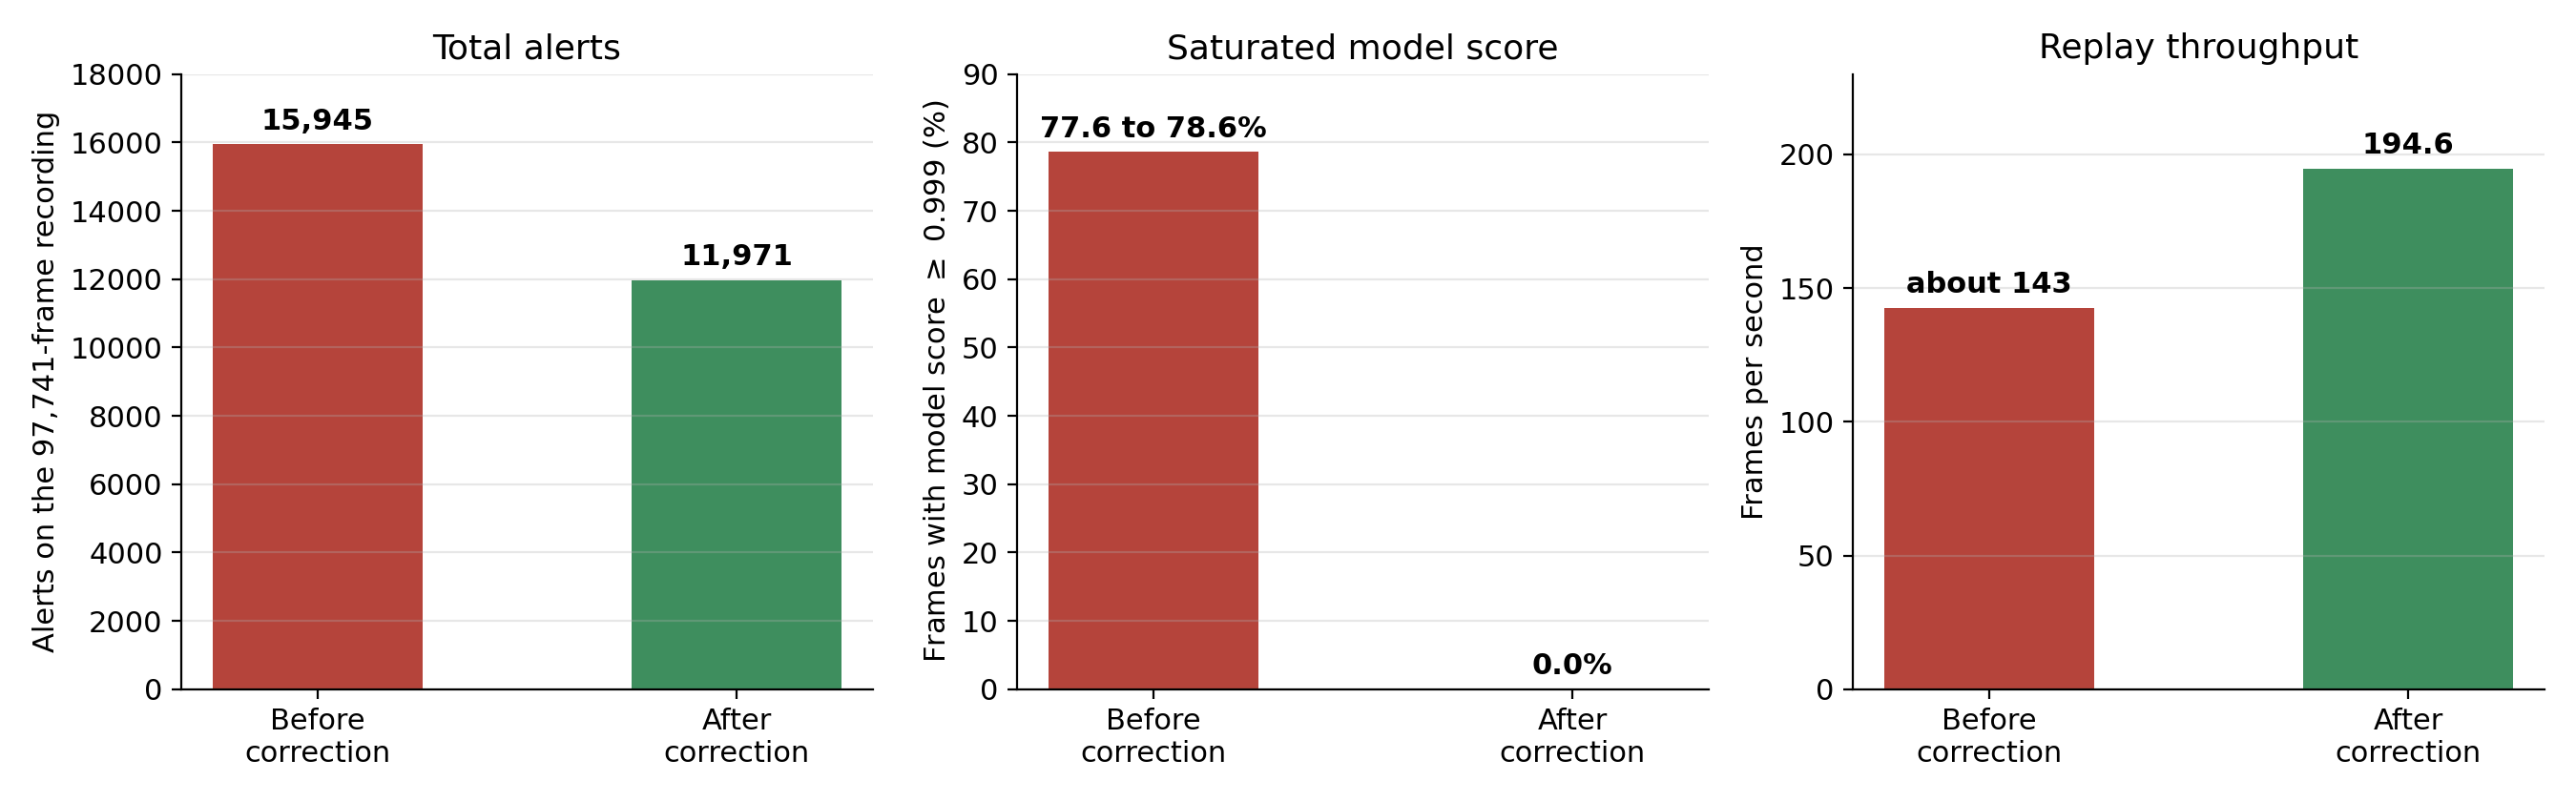
\includegraphics[width=\textwidth]{before_after_summary.png}
\caption{Alerts, saturated model score and replay throughput on the Kia EV6 recording, before and after the corrections.}
\label{fig:chart-before-after}
\end{figure}

\Needspace{278pt}% keep the text with its float
Fewer alerts and a higher throughput are side effects of fixing real defects, not of a threshold change: the right model of the vehicle replaced a saturated generic path. Figure~\ref{fig:chart-state} shows the evidence of Fix 2.

\begin{figure}[H]
\centering
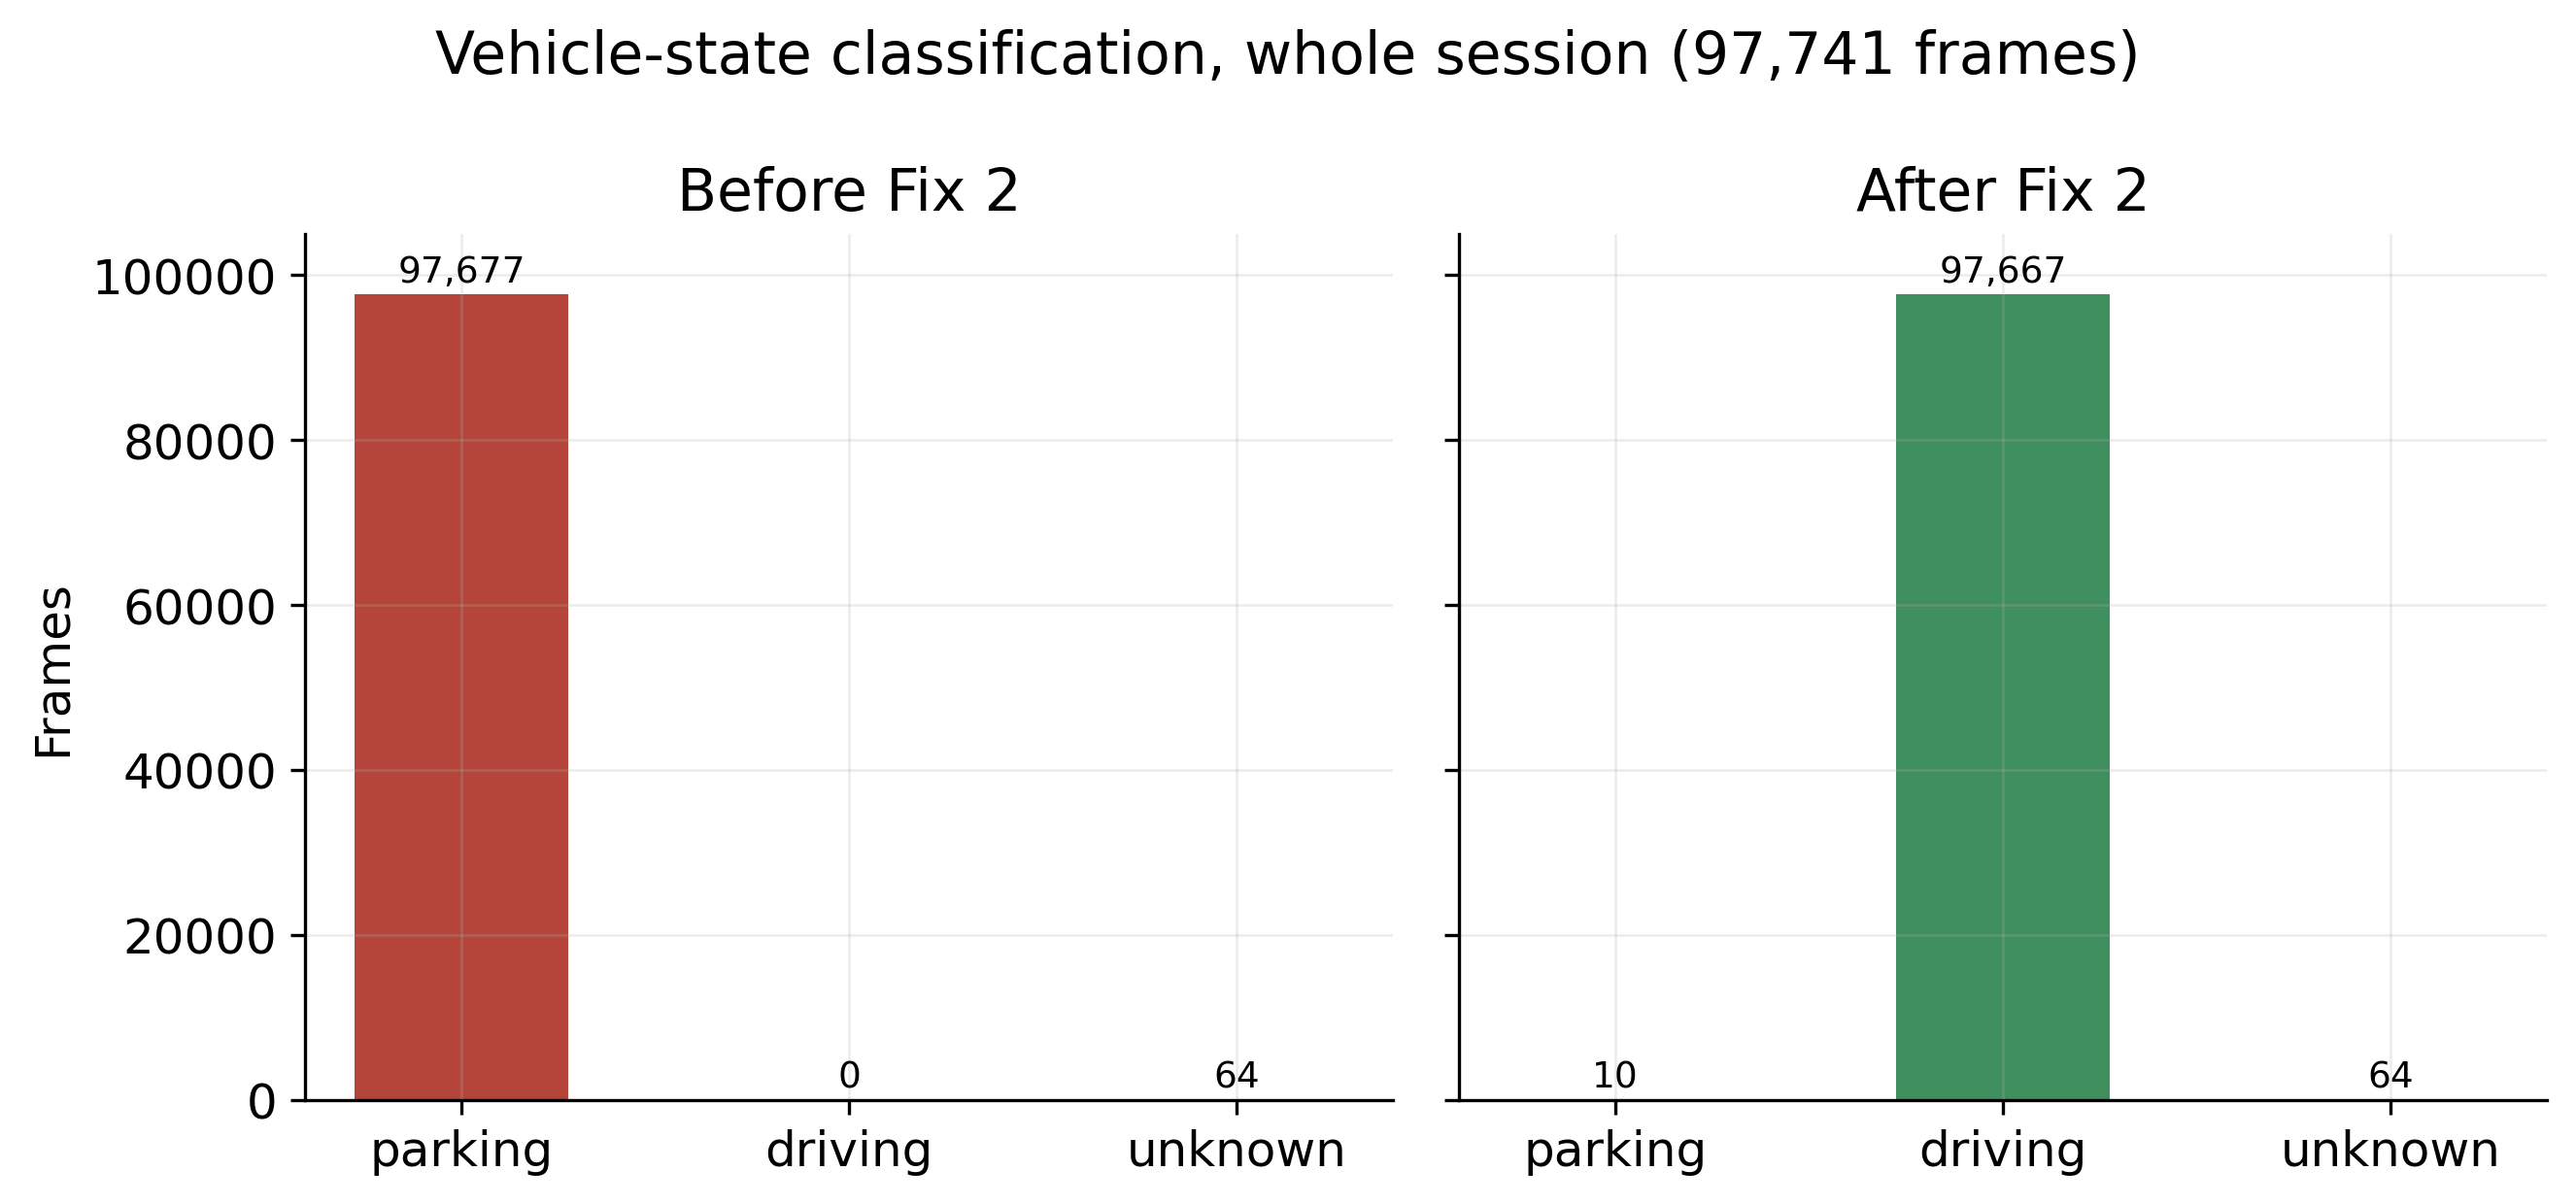
\includegraphics[width=0.85\textwidth]{state_classification_before_after.png}
\caption{Driving state of the whole recording, before and after Fix 2.}
\label{fig:chart-state}
\end{figure}

Figure~\ref{fig:chart-severity} breaks down the 11{,}971 remaining alerts. The right chart also supports Fix 3: the raw frequency and entropy no longer appear among the dominant layers.

\begin{figure}[H]
\centering
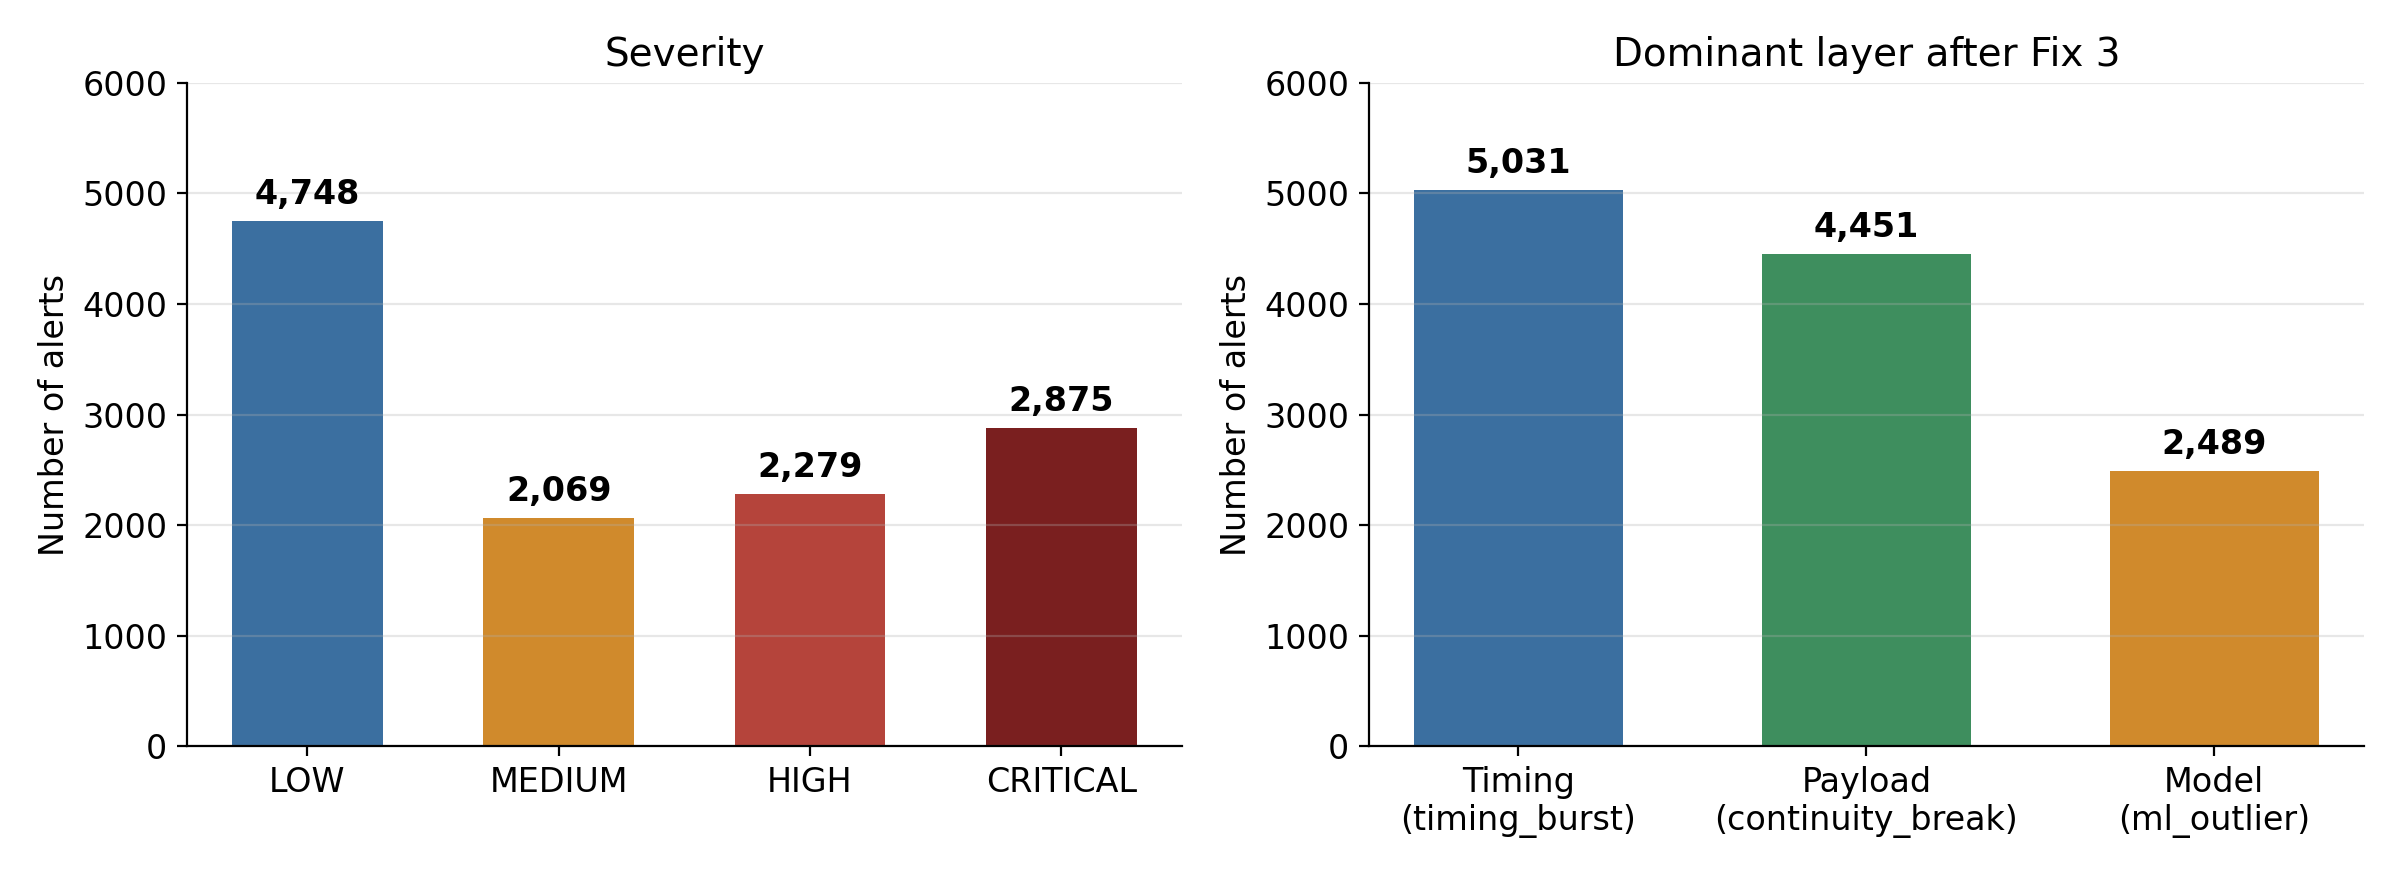
\includegraphics[width=\textwidth]{alert_breakdown.png}
\caption[Severity and dominant layer of the alerts after Fix 3.]{Severity (left) and dominant layer after Fix 3 (right) of the 11,971 alerts produced by the corrected first pipeline.}
\label{fig:chart-severity}
\end{figure}

\subsection{Assessment}

Table~\ref{tab:fixes-summary} summarises the six defects.

\begin{table}[H]
\centering
\small
\caption{Defects corrected during the second iteration.}
\label{tab:fixes-summary}
\begin{tabularx}{\textwidth}{|l|Y|c|}
\hline
\textbf{\#} & \textbf{Defect} & \textbf{Status} \\
\hline
1 & Vehicle model never used for scoring & Fixed, verified \\
\hline
2 & Driving state always classified as ``parking'' & Fixed, verified \\
\hline
3 & Diagnostic fields dominating the displayed cause (6 places) & Fixed, verified \\
\hline
4 & Replay formats other than \gls{csv} bypassing the common parser & Fixed, verified \\
\hline
5 & Polling timer left stopped after an import & Fixed, verified \\
\hline
6 & Explanation cache returning data from another session & Fixed, verified (two changes) \\
\hline
\end{tabularx}
\end{table}

All six defects were silent: none crashed or raised an error, and each appeared only when what the system reported was compared with a fact known independently, such as a vehicle being driven or a file being valid. The corrections reduced the alerts by a quarter without touching the threshold. The corrected pipeline worked, but the iteration exposed three weaknesses of its design. Two models in a chain meant that a wrong state selected the wrong forest, the source of two of the six defects. One forest per state mixed identifiers sent every 10 milliseconds with identifiers sent every second. And the fallbacks hid missing models. It was also not always possible to prove which data and settings had produced a model file. These weaknesses led to the rebuild of the models, planned as the fourth iteration, after the hardware milestone.

% ============================================================
\section{Iteration 3: hardware layer and bench rig}
\label{sec:it3}

\subsection{Objectives}

The third iteration delivered milestone M2: live capture from a physical \gls{can} adapter (FR9), and a way to test it without a vehicle, since none was available.

\subsection{Use cases addressed}

This iteration addressed the use case \emph{Connect hardware}, together with \emph{Detect anomaly}, applied to the frames of the live bus, and \emph{Record session}, which saves a live session to a log file.

\subsection{Design}
\label{sec:design-hardware}

The hardware layer wraps python-can, so it accepts the adapters python-can drives, such as slcan serial adapters, PEAK PCAN or SocketCAN, plus a virtual bus for tests. Every received frame goes to the same runtime engine as replay, built for the model chosen by the analyst, and is decoded with the \gls{dbc} file of the vehicle when it has a profile. A profile can declare its \gls{dbc} file complete, meaning that it defines every identifier of the bus, and live capture then flags any other identifier; since the \gls{dbc} files of real vehicles are partial, only a profile written for a known test bus can do so. Because the engine is shared, a bench rig test without a vehicle is meaningful for the part specific to live capture, its transport, while the engine behind it is the one that scores replays.

\subsection{Implementation}
\label{sec:impl-hardware}

Connecting an adapter builds a live engine for the model chosen by the analyst, and disconnecting stops the scoring. When no frame arrives for a few seconds, the link is reported as lost. Frames are decoded with the \gls{dbc} file of the selected profile and, with a complete profile, a frame on an identifier outside the file raises an alert on the whitelist layer.

Our bench rig replaces the vehicle. Two Arduino Uno boards, each with an MCP2515 \gls{can} module, are joined by a two wire bus terminated with 120\,$\Omega$ resistors, at 500~kbit/s. The bridge board is connected by USB and runs a small firmware that speaks the slcan protocol expected by python-can. The simulator board sends a speed frame every 20 milliseconds and a state of charge frame every 200 milliseconds, about 55 frames per second, and, from the 35th second after power on, a frame every twenty seconds on an identifier that should not exist (0x666), which the profile of the rig leaves out on purpose.

\subsection{Tests}
\label{sec:validation-bench}

Live capture was tested on the bench rig in two steps. First, a short script read the bus through python-can: the three identifiers arrived with the values of the firmware, a speed of 60~km/h and a state of charge of 78\%, which showed that both boards, the wiring and the serial link worked. Second, the rig was connected from the application (slcan, 500~kbit/s), so that the frames went through the hardware layer into the runtime engine.

This second step revealed two defects of the hardware layer, which we corrected:

\begin{itemize}
    \item \textbf{One bad line closed the session.} After about eight minutes and 16{,}304 frames received, a single malformed line on the serial link raised an error that ended the connection. One bad frame does not mean that the link is dead, so the hardware layer now skips such a line, logs it and keeps reading. After this change, the connection stayed up and received frames at about 55 per second, the rate of the firmware.
    \item \textbf{Old data stayed on screen after the rig was unplugged.} When the boards were disconnected, the link was still reported as up, because its status only changed on a hard error, and the live screens kept showing the last frames received, hours later. The link is now reported as lost when no frame has arrived for five seconds, disconnecting clears the buffers of live data, and each live update says whether it comes from the hardware or from the simulator, so that the client can show which one the analyst is looking at.
\end{itemize}

Two more gaps concerned the interpretation of live frames. First, the frames were not decoded correctly. The rig had been connected under the profile of a real vehicle, whose \gls{dbc} file does not define 0x316 or 0x3F9, and the live signal panel read the frames with a signal map shared by all vehicles, which gave them the meaning of unrelated messages from another manufacturer. Second, the frame on the unknown identifier was never raised as an alert, and it could not have been: the whitelist of \Sref{sec:design-pipeline} belonged to the offline analysis, and live capture had no check of the identifiers at all. We corrected both. The rig now has its own vehicle profile and \gls{dbc} file, and the live screens use the decoding of the selected profile first, so the live values sent to the screens become a speed of 60~km/h and a state of charge of 78\%. The profile of the rig declares its \gls{dbc} file complete, so live capture flags 0x666 on its first frame, without any learning window. Automated tests send the three frames of the rig through the virtual bus of python-can and check the decoded values, the alert on 0x666, and the absence of such alerts for a profile whose \gls{dbc} file is partial.

\subsection{Assessment}

The transport of live capture, from the bus to the runtime engine, works on the bench rig. This test does not measure detection: the traffic of the rig is synthetic and much simpler than the traffic of a vehicle. We have not yet repeated the run on the physical rig after the last corrections, and the test was made before the final models of the fourth iteration were promoted. Risk R1 remains open: live capture has not been tested on a vehicle.

% ============================================================
\section{Iteration 4: model rebuild}
\label{sec:it4}

\subsection{Objectives}

The fourth iteration rebuilt every vehicle model to remove the weaknesses found in the second iteration: one model per \gls{can} identifier instead of a chain of models, a record of how each model was built, and an evaluation on a complete recording kept out of training before any model enters production. It also measured the speed of the final models and compared Isolation Forest with the other candidate algorithms.

\subsection{Use cases addressed}

This iteration addressed the use cases \emph{Select vehicle} and \emph{Check model status}, since every model now has a status that decides what it may be used for, \emph{Detect anomaly} with the new models, and \emph{Describe capture}, which tells the analyst whether the selected model was trained or tested on the loaded file.

\subsection{Design}

\subsubsection{Final design: one model per CAN identifier}
\label{sec:impl-feature-eng}

In the final design, each vehicle has one Isolation Forest per \gls{can} identifier, with no driving state and no fallback: a frame is scored by the model of its identifier, or not at all.

\begin{itemize}
    \item \textbf{Features:} Nine features are computed over a short window of recent frames of the identifier: the time since the previous frame with its rolling mean and standard deviation, the byte difference with the previous frame with its rolling mean, standard deviation and maximum, the number of changed bytes, and the payload entropy. A feature that never changes for an identifier is dropped for it. The same code computes the features for training, offline analysis and live scoring.
    \item \textbf{Unscored frames:} An identifier needs 1{,}000 training rows to get a model; below that it is \emph{sparse}, an identifier whose features never vary is \emph{unmodelled}, and one absent from training is \emph{unseen}. Their frames, and the first frames of any identifier (\emph{warmup}), are reported as unresolved with their reason, so the analyst sees how much of a recording the models covered.
    \item \textbf{Threshold:} Each model has its own threshold, set so that 2\% of its training rows are flagged. The raw score is mapped to a normalised score: 0 at the median of the training rows, 0.5 at the threshold, closer to 1 as the frame becomes more anomalous. The 2\% value was fixed before any test recording was scored and never changed afterwards.
\end{itemize}

\Needspace{162pt}% keep the text with its float
Table~\ref{tab:model-params} lists the parameters, also recorded in the manifest of every model.

\begin{table}[H]
\centering
\small
\caption{Parameters of the final models.}
\label{tab:model-params}
\begin{tabularx}{\textwidth}{|P{3.6cm}|Y|}
\hline
Forest & scikit-learn Isolation Forest, 200 trees, random seed 42, no feature scaling (a tree splits on one feature at a time) \\
\hline
Window and warmup & The last 10 frames of the identifier; its first 10 frames are not scored \\
\hline
Minimum data & 1{,}000 training rows per identifier \\
\hline
Threshold & With $n$ training rows and $k = \lfloor 0.02\,n \rfloor$, the $(k+1)$th smallest raw score; a frame is flagged below it \\
\hline
\end{tabularx}
\end{table}

\subsubsection{Training and promotion pipeline}

Figure~\ref{fig:ml-training} shows how the models are produced. The corpus of each vehicle is split by recording, not by frame: at least one complete recording is kept aside as a \emph{holdout}, never used to fit the model or set its threshold, because two frames of the same recording are too similar for a frame level split to say anything about a new recording. The SHA-256 fingerprint of each file guarantees that no recording is used on both sides.

A training run writes the models into a staging folder with a \emph{manifest} that records the code versions, the Git commit, the parameters, the threshold, median and row count of each identifier, and the SHA-256 fingerprints of the model file and of every recording. When the backend loads a vehicle, it checks that the model file and the manifest agree and that no recording is on both sides, and refuses the model otherwise. After the holdout evaluation, the promotion step copies accepted models to production and archives the previous files.

\begin{figure}[H]
\centering
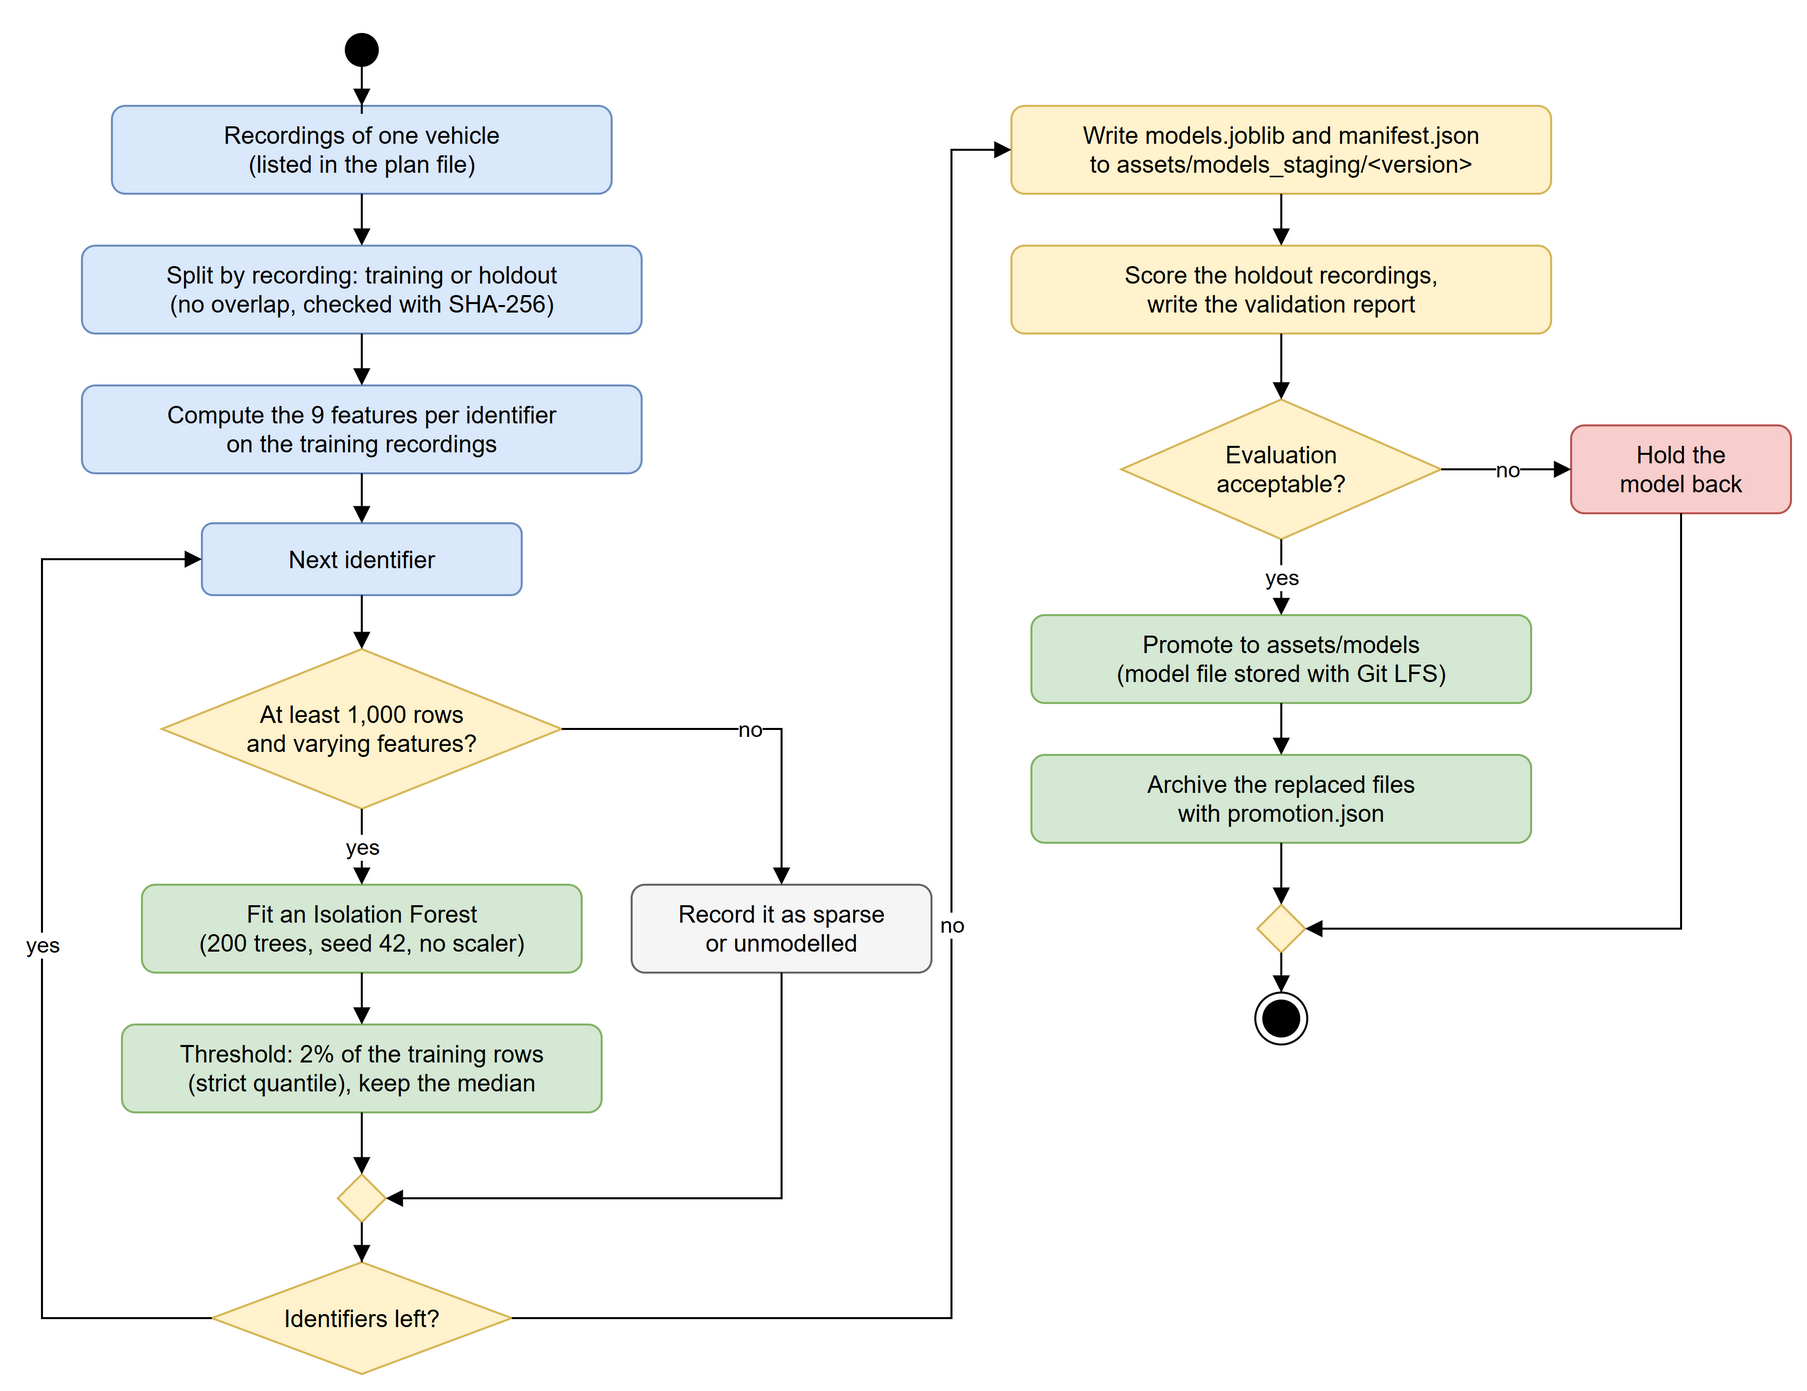
\includegraphics[width=\textwidth]{ml_training_pipeline.png}
\caption{Training pipeline, from the recordings of a vehicle to a model in production.}
\label{fig:ml-training}
\end{figure}

\Needspace{347pt}% keep the text with its float
\Needspace{133pt}% keep the heading with its float
\subsubsection{Model status}

Some vehicles have a single recording, so no holdout exists, and some models fail their evaluation. Each model therefore has a status that decides what it may be used for (Table~\ref{tab:model-status}), and the client shows it next to each model. Figure~\ref{fig:state-model-status} shows the life cycle of a model under the new pipeline as a state diagram.

\begin{table}[H]
\centering
\caption{Status of a model and what it allows.}
\label{tab:model-status}
\begin{tabularx}{\textwidth}{|P{4.6cm}|Y|}
\hline
\textbf{Status} & \textbf{Meaning and use} \\
\hline
Evaluated on a holdout & Final model in production. Used offline and live. \\
\hline
Not validated, no holdout & A final model exists, but the vehicle has only one recording. Refused offline; live capture uses the model of the first design, with a visible label. \\
\hline
Held back & Failed its evaluation. Refused offline and live. \\
\hline
No final model & No model could be built under the new rules. Refused. \\
\hline
Legacy & Only a model of the first design exists. Refused offline; accepted live with a visible label. \\
\hline
General & The general model of the first design, for a vehicle without its own model. \\
\hline
\end{tabularx}
\end{table}

\begin{figure}[H]
\centering
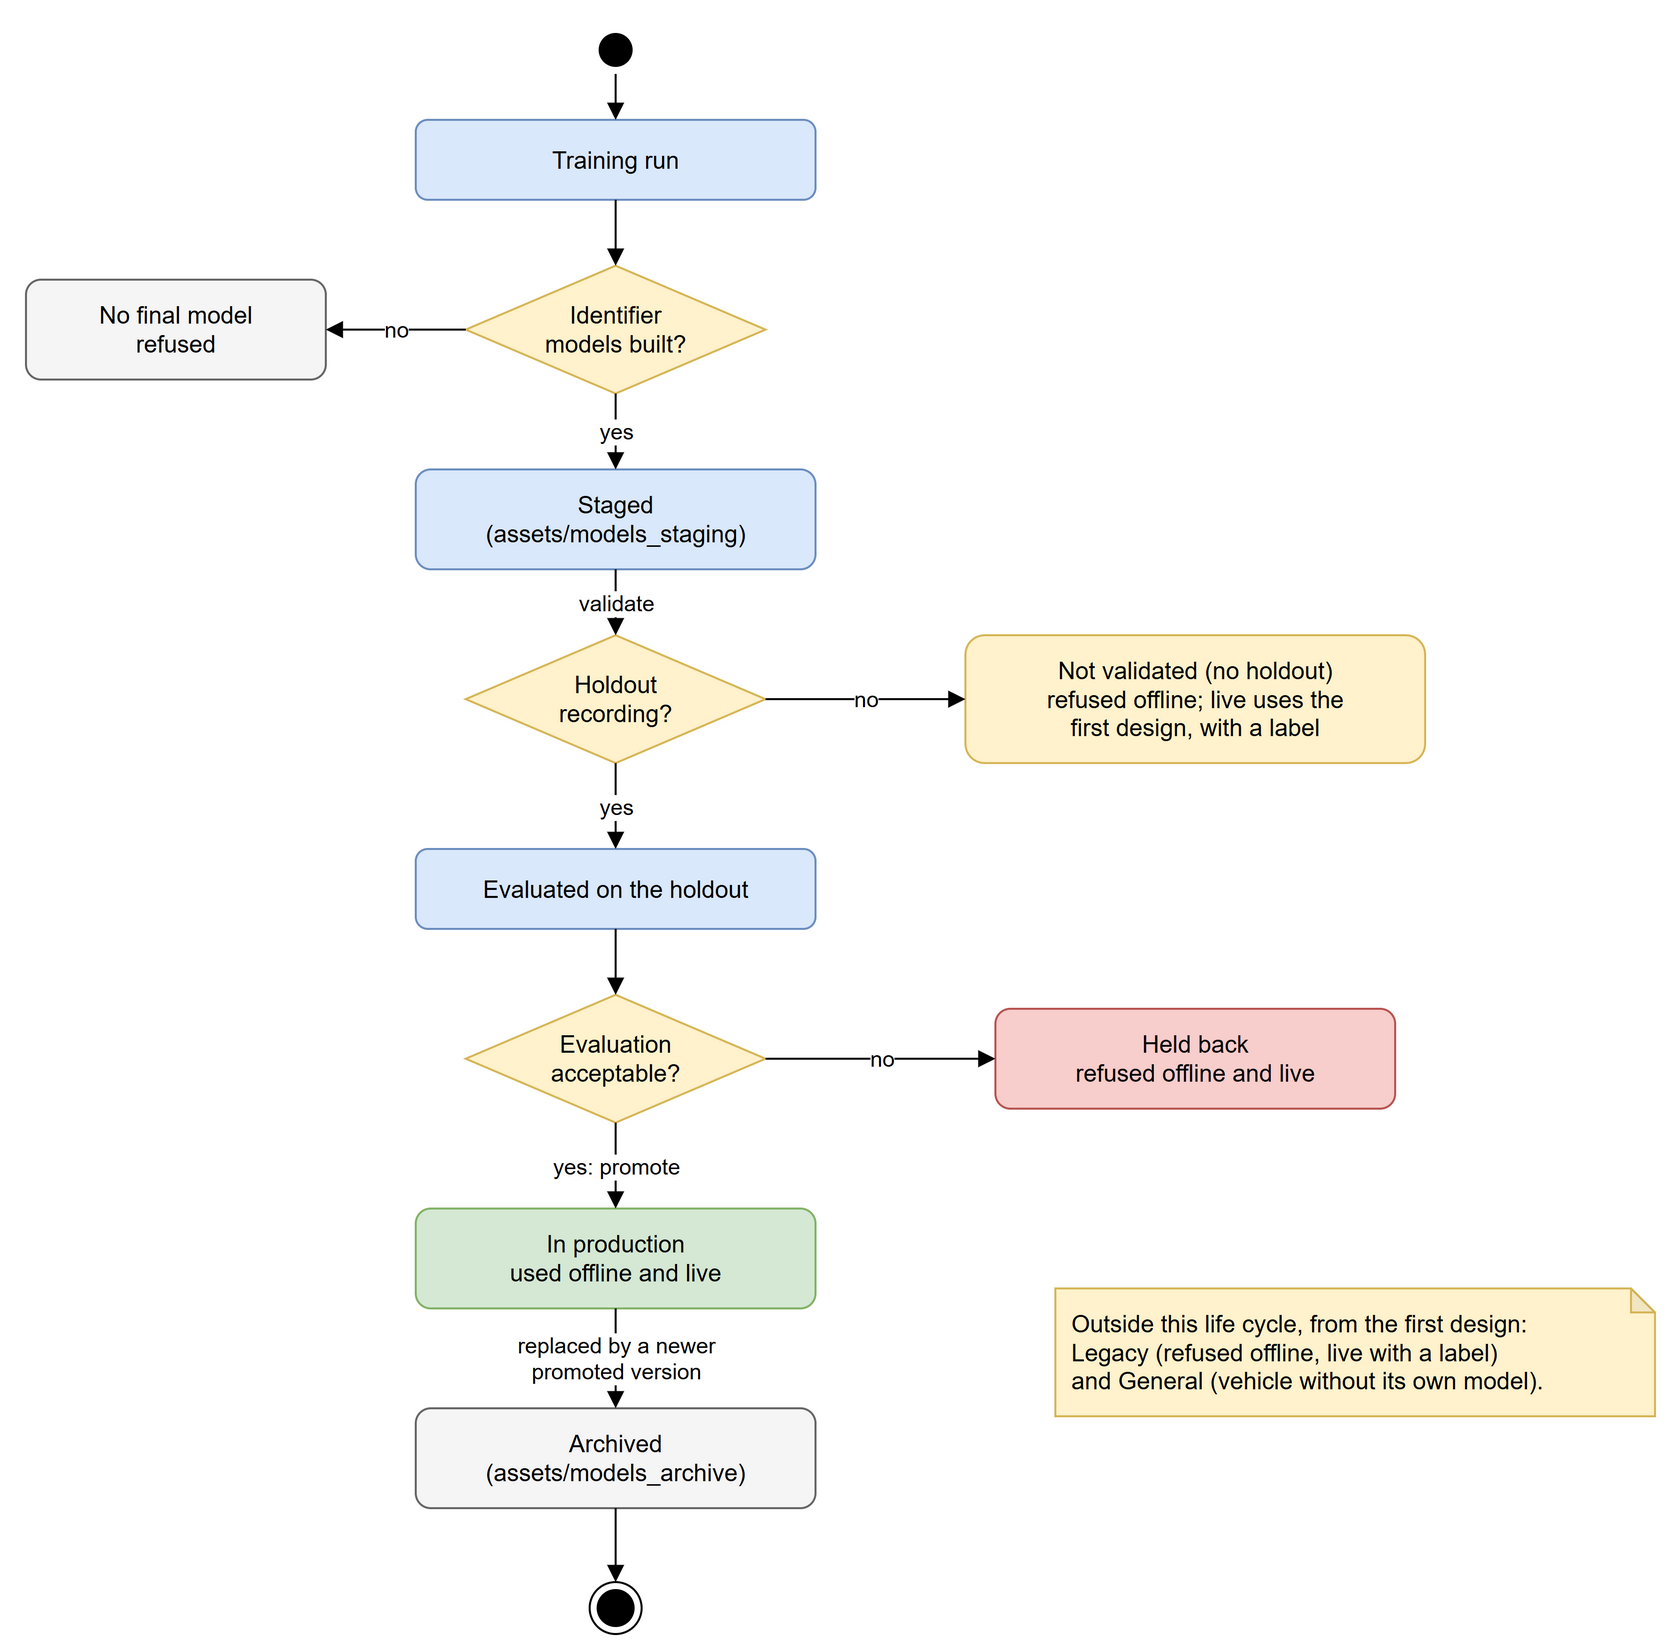
\includegraphics[height=0.62\textheight]{state_model_status.png}
\caption{State diagram: life cycle of a vehicle model.}
\label{fig:state-model-status}
\end{figure}

\subsection{Implementation}
\label{sec:impl-models}

The training pipeline is a set of Python scripts driven by a plan file that lists the training and holdout recordings of each vehicle. Its commands check the corpus and print the split without fitting anything, train a version into the staging folder, validate a staged version, and promote it. A run produces a validation report, read before any promotion; the promotion script refuses a held back vehicle and archives the files it replaces. The model files are stored with Git LFS.

At run time, one resolver gives the status of every model to the offline analysis, the live capture and the model list of the client, so they never disagree, and a model that may not be used is refused with an explicit reason instead of being replaced. The live engine of the hardware layer goes through the same resolver, so a held back or unknown model is refused for live capture too.

\label{sec:impl-capture}
The manifests also describe the recordings. The dataset card of the client sends the fingerprint of the loaded file to the backend, which looks it up in the manifest of the selected model and answers whether the model was trained on this file, tested on it, or never saw it. For the signals of a capture (FR12), the backend keeps the decoded signals that really change when a \gls{dbc} file exists, and ranks speed, state of charge, voltage, current and temperatures first; without one, it shows the raw payload bytes that change smoothly, as a physical value does, leaves out constants and rolling counters, and labels every raw channel as undecoded.

\subsection{Tests}

\subsubsection{Evaluation protocol}
\label{sec:validation-protocol}

Each final model was scored on every frame of its holdout recording, counting the frames scored, the frames flagged, and the frames that could not be scored, with their reason.

The holdout recordings carry no attack labels; we assume that they contain normal traffic but cannot prove it. We therefore report a \emph{flagged rate}, the share of scored frames that the model flagged, and not a false positive rate, a precision or a recall. If a holdout recording is entirely normal, every flagged frame in it is a false alarm and the flagged rate is the false alarm rate; if it is not, the flagged rate also contains real anomalies. Since each threshold flags 2\% of the training frames by construction, a flagged rate close to 2\% on a new recording means that the model sees this recording roughly as it saw its training data.

\subsubsection{Holdout results}

Table~\ref{tab:holdout-results} gives the results of the four models put into production. Together, they were trained on 23 recordings (3{,}436{,}061 frames) and evaluated on 1{,}130{,}500 frames of other recordings.

\begin{table}[H]
\centering
\footnotesize
\setlength{\tabcolsep}{4pt}
\caption{Final models scored on their holdout recordings.}
\label{tab:holdout-results}
\begin{tabular}{|l|r|r|r|r|r|r|}
\hline
\textbf{Vehicle} & \textbf{ID models} & \textbf{Training frames} & \textbf{Holdout frames} & \textbf{Scored} & \textbf{Flagged / scored} & \textbf{Rate} \\
\hline
Jaguar I-PACE & 46 & 233{,}598 & 50{,}361 & 82.6\% & 1{,}249 / 40{,}477 & 3.09\% \\
\hline
Kia EV6 & 161 & 448{,}198 & 438{,}170 & 98.4\% & 11{,}109 / 429{,}524 & 2.59\% \\
\hline
Nissan Leaf 2019 & 12 & 1{,}317{,}070 & 491{,}969 & 100.0\% & 2{,}951 / 491{,}797 & 0.60\% \\
\hline
ROAD ambient & 77 & 1{,}437{,}195 & 150{,}000 & 99.0\% & 8{,}982 / 147{,}485 & 6.09\% \\
\hline
\end{tabular}
\normalsize
\end{table}

The holdout recordings are \texttt{canbus\_turningon\_quickly.csv} for the Jaguar I-PACE, \texttt{Vehicle everthing on.asc} for the Kia EV6 (the spelling is the one of the original file), \texttt{00000001-61D9D9BA.MF4} for the Nissan Leaf 2019, and the first 150{,}000 frames of \texttt{ambient\_highway\_street\_driving\_long.log} for the ROAD vehicle. The \emph{Scored} column is the share of frames that belong to an identifier with a model, after warmup. The Jaguar I-PACE has the lowest coverage: on its holdout file, 8{,}451 frames belong to sparse identifiers, 1{,}368 are warmup frames and 65 belong to unseen identifiers, all reported as unresolved rather than normal.

We read these results as follows.

\begin{itemize}
    \item \textbf{Nissan Leaf 2019 (0.60\%).} The model flags fewer frames on its holdout than on its training data. The holdout comes from the same logger as the training recordings, and the model sees it as ordinary traffic.
    \item \textbf{Jaguar I-PACE (3.09\%) and Kia EV6 (2.59\%).} Both rates are close to the 2\% of the calibration, slightly above it, which is what we expected for a new session of the same vehicle.
    \item \textbf{ROAD ambient (6.09\%).} This rate is three times the calibration level. Most of the difference comes from one identifier, 0x193: its payload never changes in any training recording, but it does change on the highway recording used as holdout, and 58\% of its holdout frames are flagged. This is a difference of coverage between training and holdout, not a problem of threshold. We did not change the threshold after seeing the holdout, since this would have turned the holdout into training data.
\end{itemize}

\subsubsection{Models we did not put into production}

The same protocol showed which models not to trust. The MG ZS EV model flagged 43.60\% of the scored frames of its holdout, because about 78\% of its holdout frames belong to identifiers absent from its only training recording; it was held back. Three other model families (the Hyundai Ioniq 5, a Tesla and a Kaggle dataset of normal traffic) have a single recording, so their models are marked as not validated and refused by the offline analysis, and for two vehicles no final model could be built (Table~\ref{tab:model-status}).

\subsubsection{Consistency checks}

For every identifier model, the threshold recomputed from the training rows matched the manifest (rows, $k$, threshold, flagged rows and median), and the fingerprints confirmed that no recording is both in the training set and in the holdout of a vehicle.

\subsubsection{Speed of the final models}
\label{sec:validation-speed}

A benchmark replayed the first 10{,}000 frames of each holdout through the runtime engine, as live capture would (Table~\ref{tab:perf-live}).

\begin{table}[H]
\centering
\caption{Speed of the live path with the final models, on the first 10,000 frames of each holdout. The model call is given as mean and 99th percentile.}
\label{tab:perf-live}
\begin{tabular}{|l|>{\raggedleft\arraybackslash}p{2.2cm}|>{\raggedleft\arraybackslash}p{2.4cm}|>{\raggedleft\arraybackslash}p{2cm}|>{\raggedleft\arraybackslash}p{2.2cm}|}
\hline
\textbf{Vehicle} & \textbf{Bus (frames/s)} & \textbf{Processed (frames/s)} & \textbf{Real time factor} & \textbf{Model call (ms)} \\
\hline
Jaguar I-PACE & 2{,}990 & 262 & 0.09 & 23.6 / 32.7 \\
\hline
Kia EV6 & 448 & 224 & 0.50 & 23.5 / 33.8 \\
\hline
Nissan Leaf 2019 & 98 & 205 & 2.10 & 23.8 / 34.6 \\
\hline
ROAD ambient & 2{,}391 & 219 & 0.09 & 23.7 / 34.7 \\
\hline
\end{tabular}
\end{table}

One model call costs about 24 milliseconds, so even with the model called on every fifth frame, the live path processes about 200 to 260 frames per second. It keeps up with the Nissan Leaf (about 100 frames per second) but not with the Jaguar I-PACE or the ROAD vehicle (thousands per second), and reaches half of the Kia EV6 rate. The offline analysis scores whole batches: the 491{,}969 frames of the Leaf holdout took 187 seconds, and the Jaguar file 16 seconds in the backend and about one minute in the application. NFR1 is therefore met offline, and live only for slow buses.

\Needspace{396pt}% keep the heading with its float
\subsubsection{Comparison with the other candidate algorithms}
\label{sec:validation-compare}

As planned in \Sref{sec:ml-selection}, we measured LOF and the One Class SVM against Isolation Forest under the same conditions (Figure~\ref{fig:ml-compare-pipeline}). The four vehicles with a final model keep their production split, and every identifier with a final model is fitted three times, on the same features and the same training rows: at most 5{,}000 evenly spaced rows per identifier, because the One Class SVM does not scale to the largest ones. The three models get the threshold rule of the final models and score the holdout recording, which none of them saw.

\begin{figure}[H]
\centering
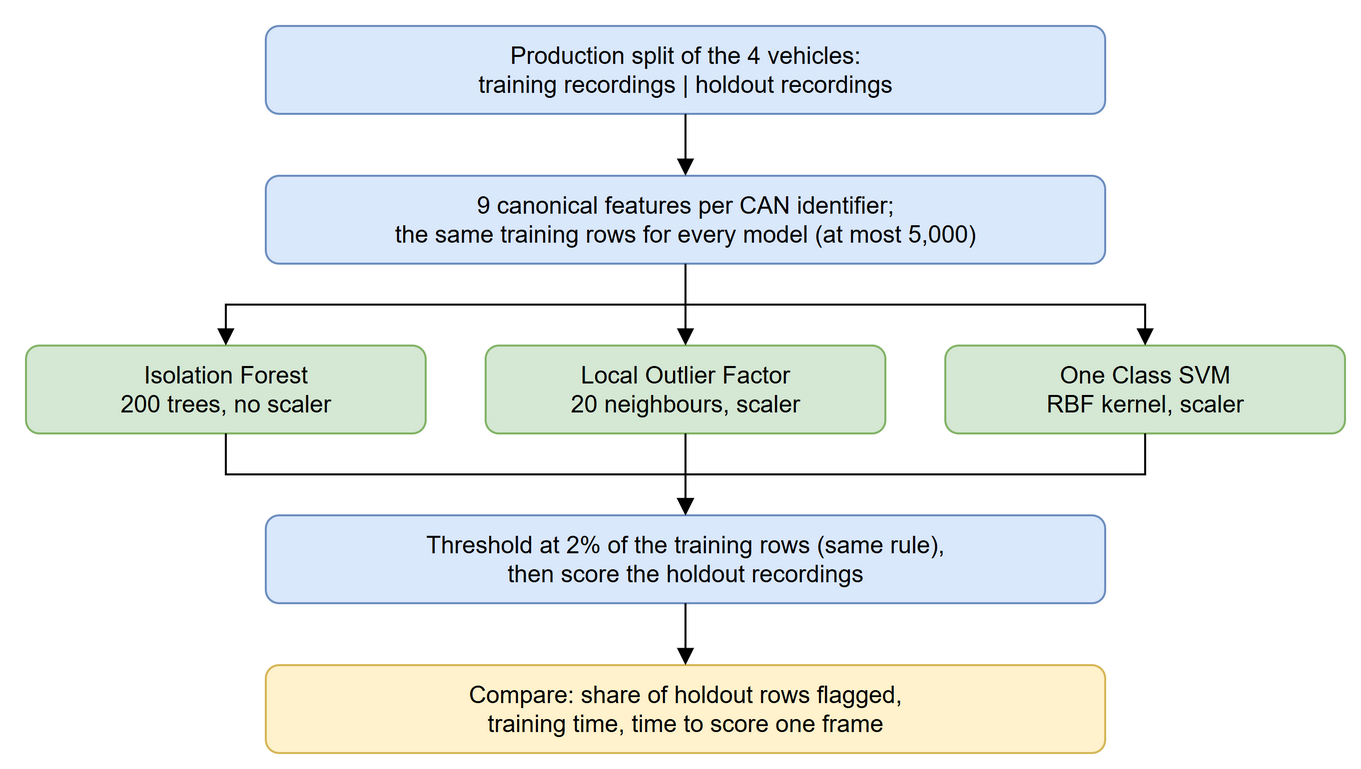
\includegraphics[width=0.8\textwidth]{ml_comparison_pipeline.png}
\caption[Pipeline of the algorithm comparison.]{Pipeline of the comparison: the same split, features, training rows and threshold rule for the three algorithms.}
\label{fig:ml-compare-pipeline}
\end{figure}

There are no attack labels, so the measure comes from the holdout recordings, which we assume to be normal traffic (\Sref{sec:validation-protocol}): every flagged row is then a false alarm, and a model whose boundary generalises flags about the 2\% of its calibration. Isolation Forest flags the fewest normal rows on average, 3.2\% against 5.1\% for LOF and 6.5\% for the One Class SVM, and has the lowest worst case, 6.4\% on ROAD against 13.1\% and 14.0\% on the Jaguar I-PACE (Figure~\ref{fig:ml-compare-flagged}). It is not the best everywhere: LOF does as well on the Kia EV6 and better on ROAD. Trained on these capped rows, Isolation Forest stays close to the final models trained on all rows (Table~\ref{tab:holdout-results}).

\begin{figure}[H]
\centering
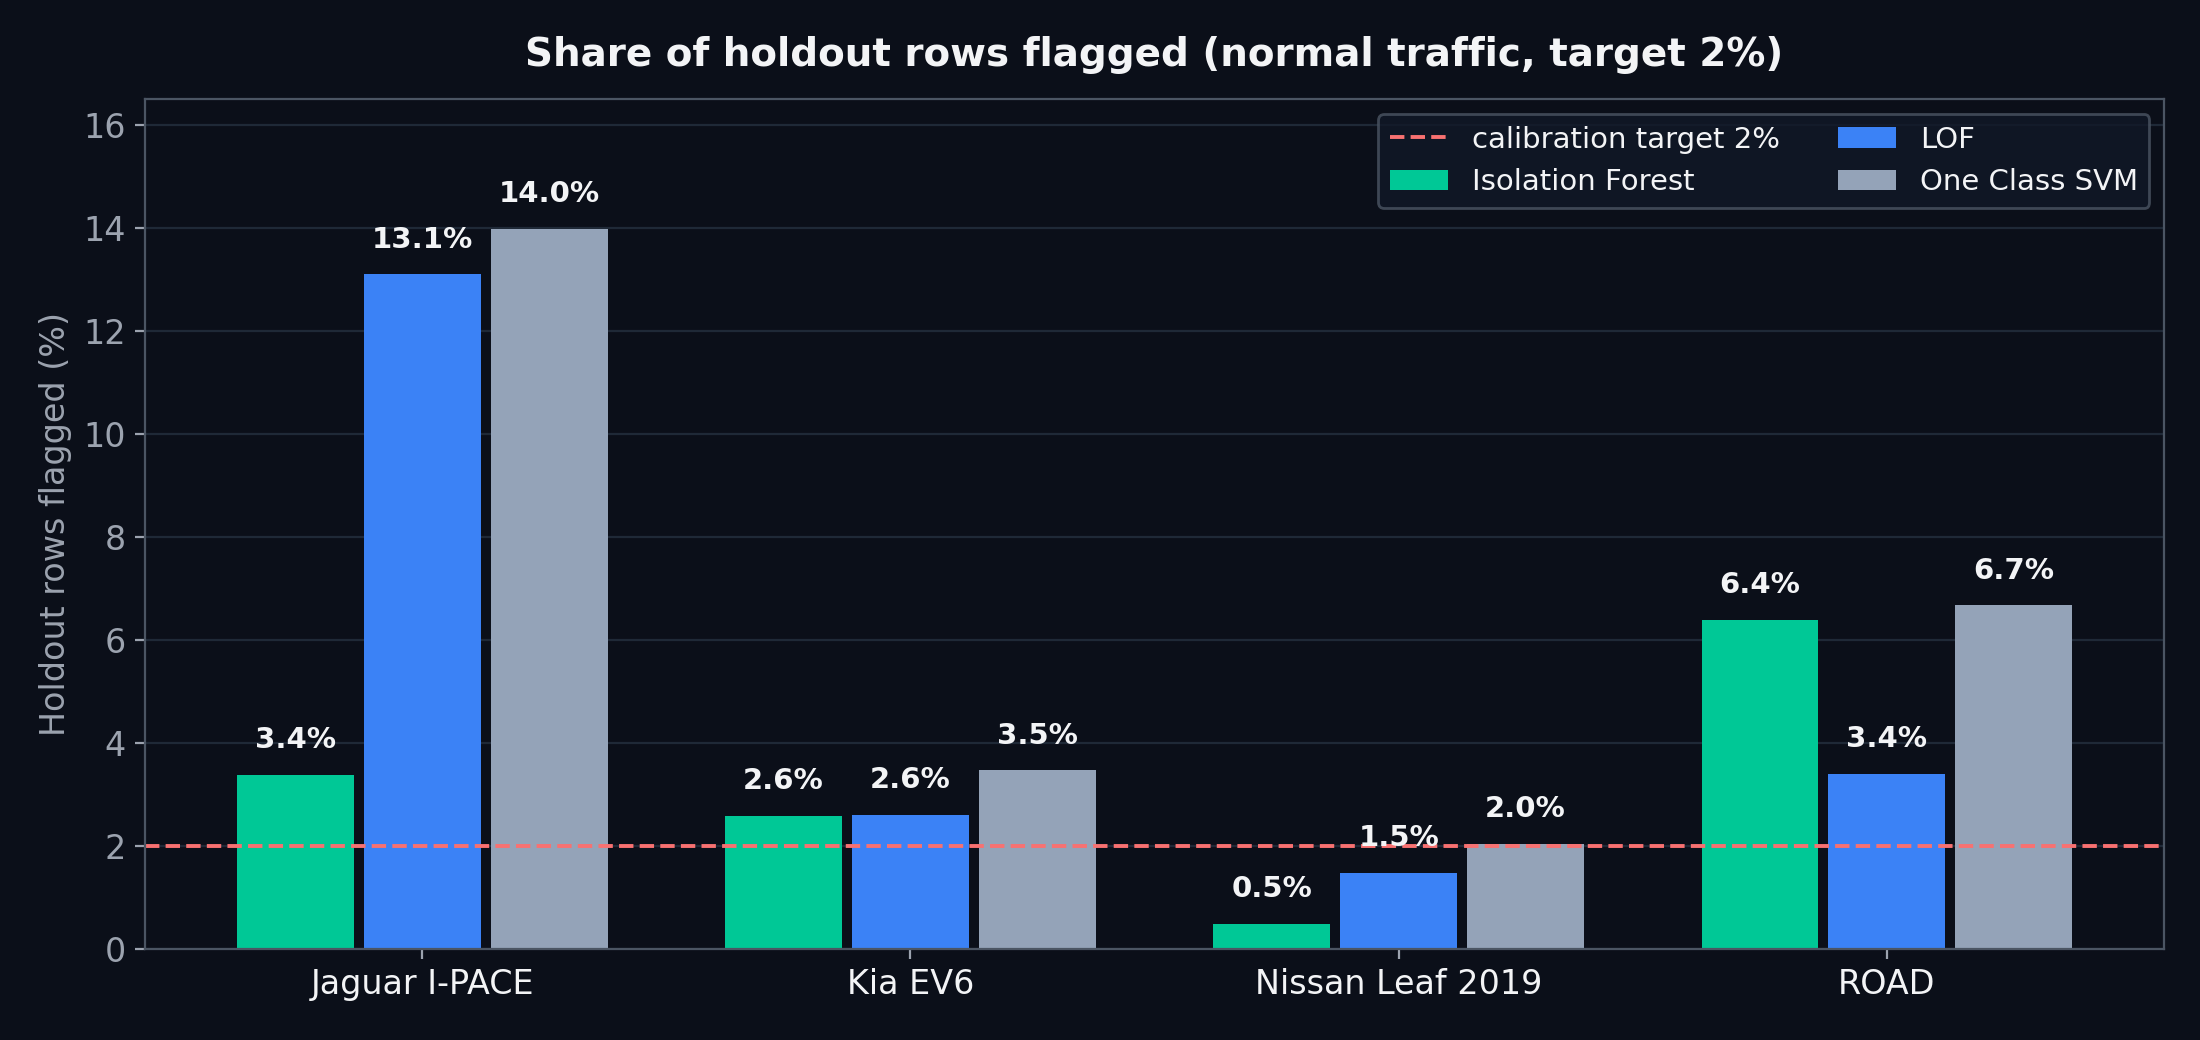
\includegraphics[width=\textwidth]{ml_compare_flagged.png}
\caption[Share of the holdout rows flagged by each algorithm.]{Share of the holdout rows flagged by each algorithm. The holdouts are assumed to be normal traffic, so a flagged row counts as a false alarm.}
\label{fig:ml-compare-flagged}
\end{figure}

This advantage has a price (Figure~\ref{fig:ml-compare-cost}). Isolation Forest is the slowest of the three: 138 seconds of training for the four vehicles against 41 and 17, and about 23 milliseconds to score one frame against 1 and 0.4. This is the model call measured in \Sref{sec:validation-speed}, and the reason the live path does not keep up with fast buses. We kept Isolation Forest because the offline analysis, the main use of the platform, needs few and even false alarms more than speed; LOF would score a live frame more than twenty times faster, at the cost of four times more false alarms on the Jaguar I-PACE.

\begin{figure}[H]
\centering
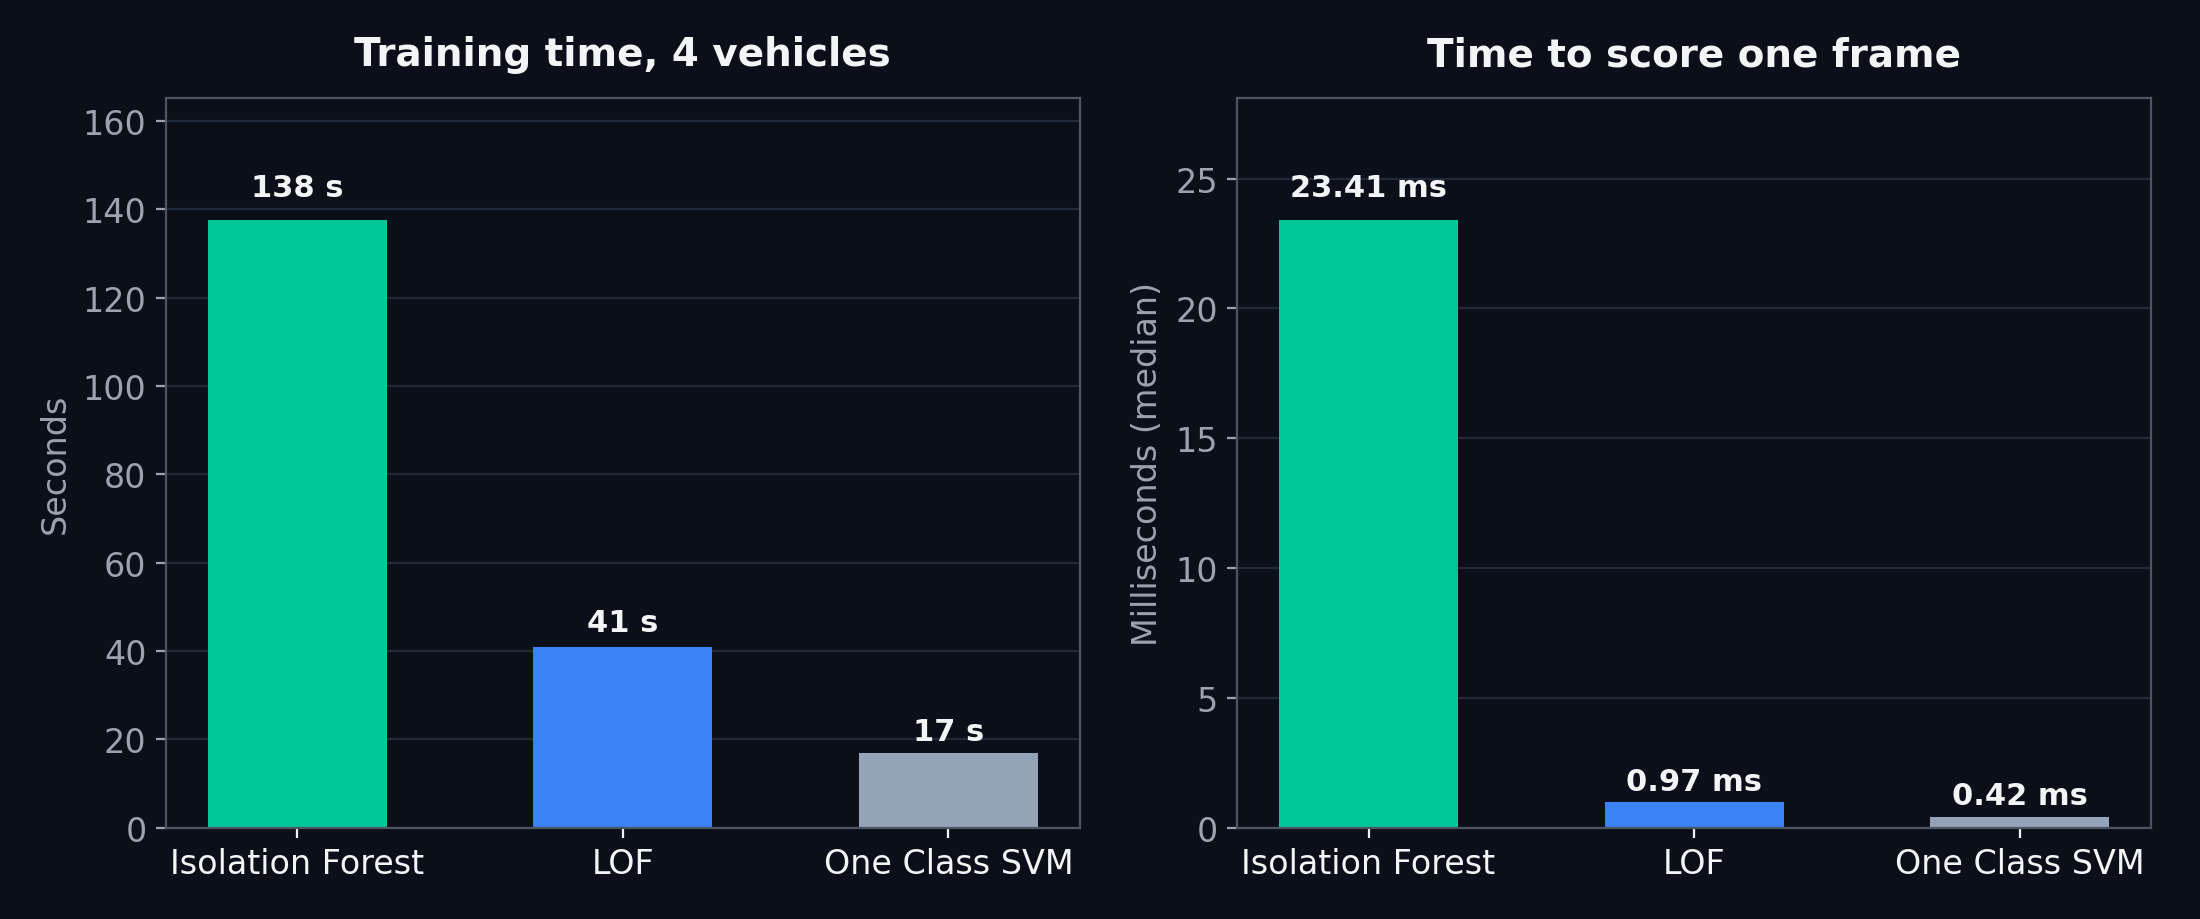
\includegraphics[width=\textwidth]{ml_compare_cost.png}
\caption[Training time and time to score one frame.]{Training time for the four vehicles, and median time to score one frame.}
\label{fig:ml-compare-cost}
\end{figure}

\Needspace{321pt}% keep the text with its float
Figure~\ref{fig:ml-feature-shares} shows what the final forests rely on. The three timing features carry about two thirds of the splits (64\%) and the six payload features the rest: for most identifiers, the sending rhythm is what isolates an unusual frame first.

\begin{figure}[H]
\centering
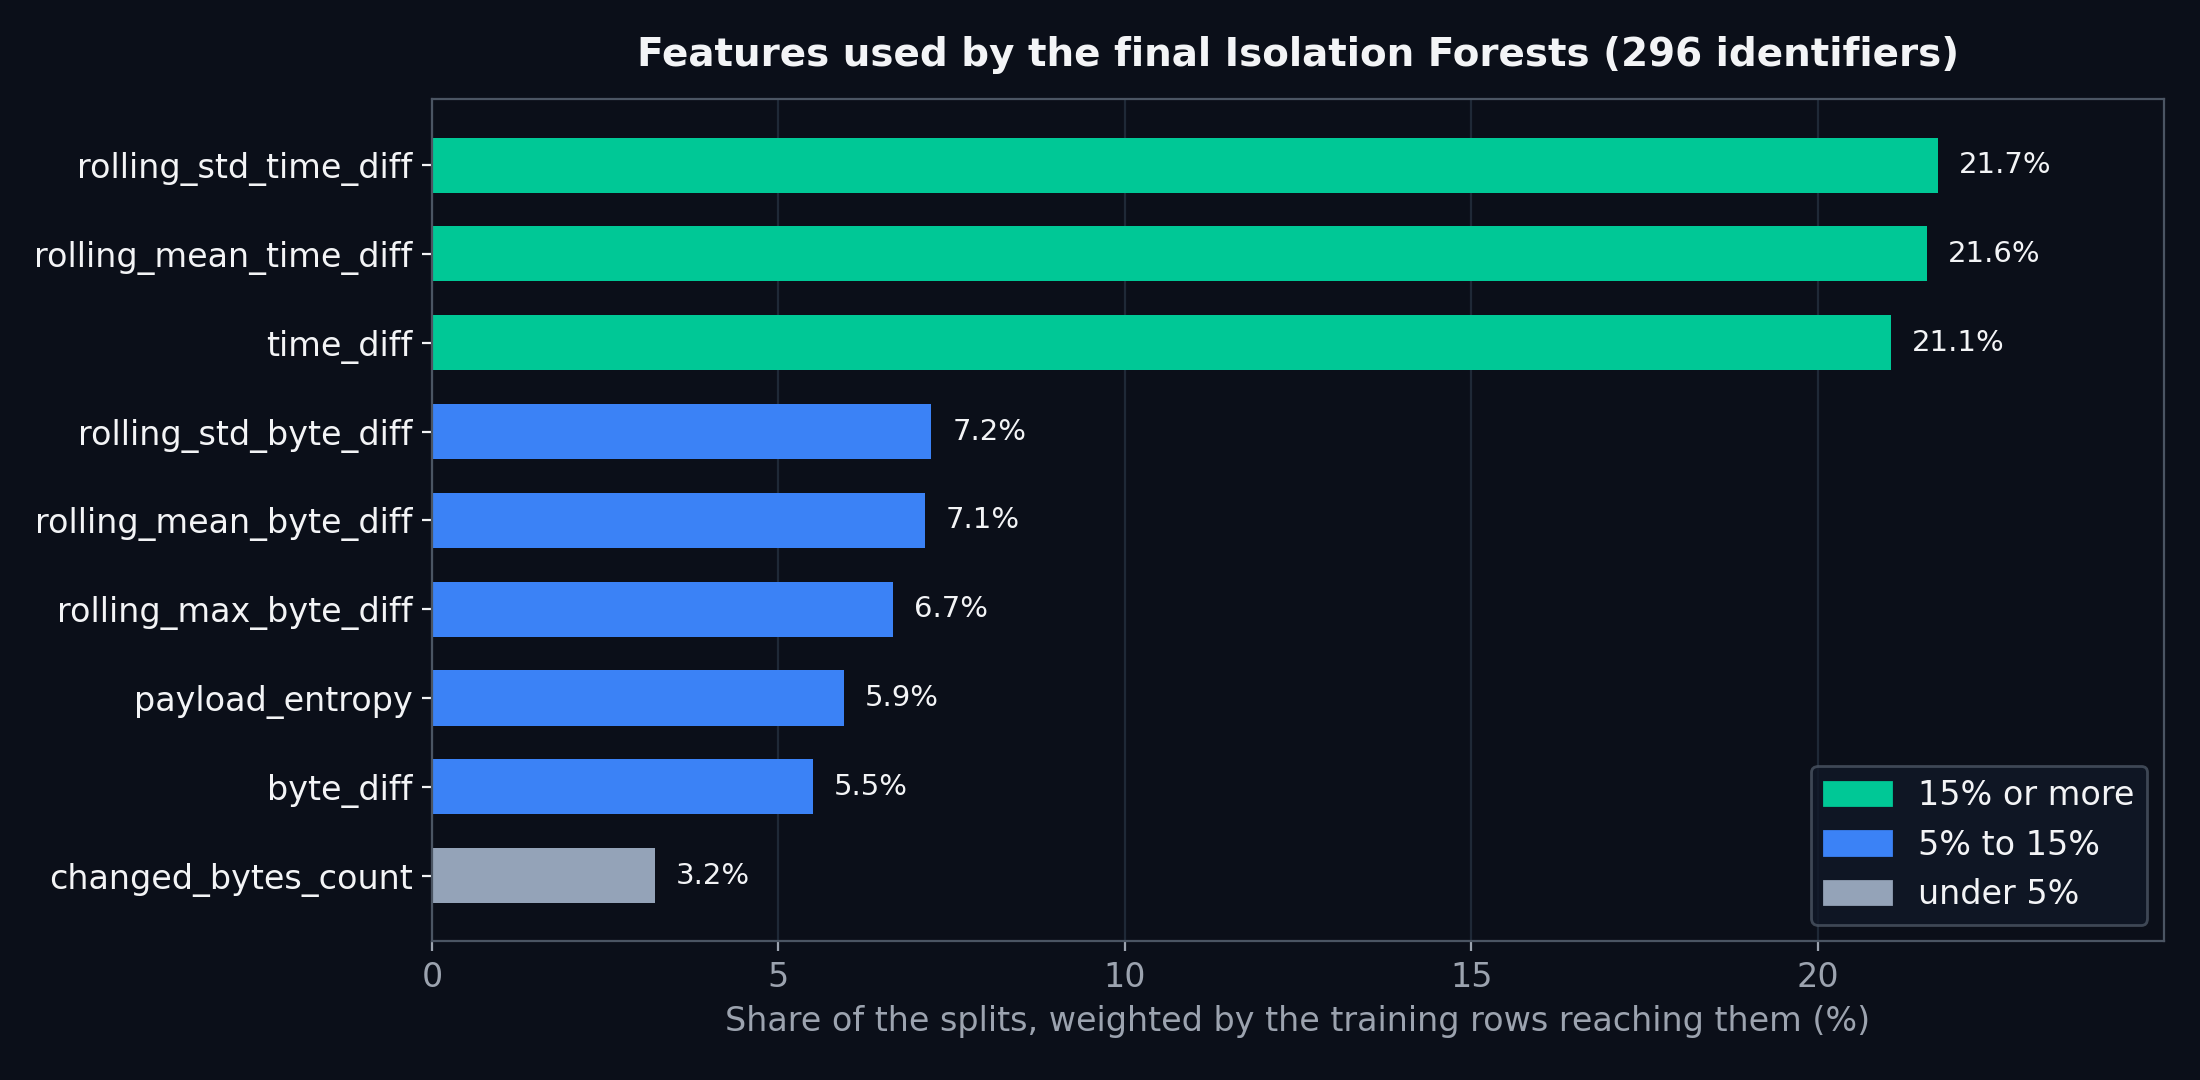
\includegraphics[width=\textwidth]{ml_feature_shares.png}
\caption[Features used by the final Isolation Forests.]{Features used by the final Isolation Forests: share of the splits, weighted by the training rows that reach them, averaged over the 296 identifier models.}
\label{fig:ml-feature-shares}
\end{figure}

\subsection{Assessment}

Four vehicles are in production, with 296 identifier models, each evaluated on a recording it never saw, with flagged rates from 0.60\% to 6.09\% that could each be explained. One model, the MG ZS EV, was held back because its evaluation showed that it could not be trusted. Isolation Forest was confirmed as the algorithm that flags the fewest normal rows, at the cost of a live path limited to slow buses.

\section*{Conclusion}
\addcontentsline{toc}{section}{Conclusion}

The four iterations of the construction phase delivered the first detection pipeline and the client, validated and corrected it on a real recording, added live capture tested on a bench rig, and rebuilt the models so that each one enters production only after an evaluation on unseen data. The next chapter presents the transition phase: the final release, its tests and its deployment.

\chapter{Transition: Final Release and Validation}
\label{chap:transition}

\section{Introduction}

The transition phase delivers the system to its users. This chapter presents the final release use case by use case, the test strategy and its results, the traceability of the requirements, the installation and documentation of the platform, and the scope within which it can be considered stable.

\section{Final application tour}
\label{sec:tour}

The screenshots below show the final release during the analysis of the Jaguar I-PACE holdout recording, a file the Jaguar I-PACE model never saw during its training. The title bar shows the short name of the application, CANvision.

\begin{itemize}
    \item \textbf{Import log:} Every session starts on the Home screen, with the choice between a live session and an offline import (Figure~\ref{fig:screen-home}). The live session stays locked until the backend runs and a USB adapter, such as an Arduino board, is plugged in. Importing a log leads to the choice of the vehicle model, with the status of each model.
\end{itemize}

\begin{figure}[H]
\centering
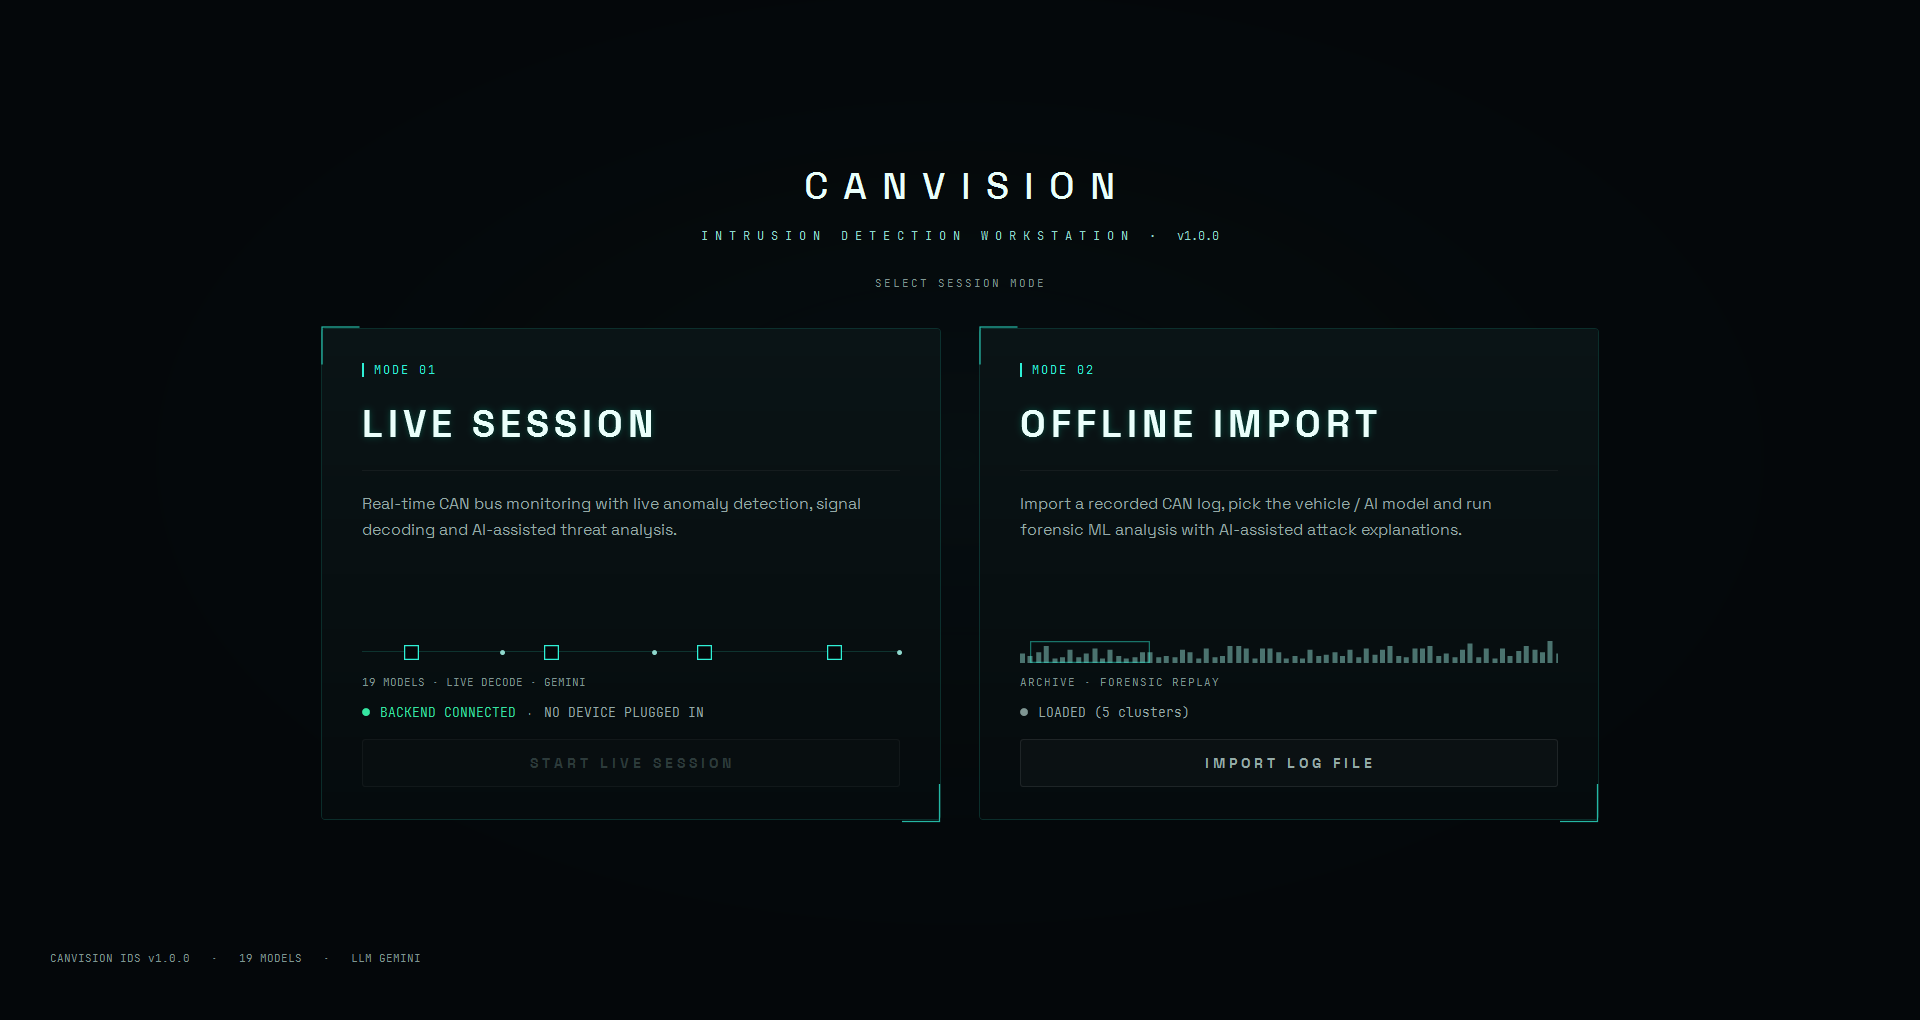
\includegraphics[width=0.72\textwidth]{f01_home.png}
\caption{Home screen: choice between a live session and an offline import.}
\label{fig:screen-home}
\end{figure}

\begin{itemize}
    \item \textbf{Detect anomaly and review the results:} After the analysis, the Dashboard (Figure~\ref{fig:screen-dashboard-final}) shows the highest flagged score, the number of alerts, the share of scored frames that were flagged, the unresolved frames with their reasons, the trend of the scores and the bus monitor. For this file, the application read 50{,}361 frames, scored 40{,}477 and flagged 1{,}249, the 3.09\% of Table~\ref{tab:holdout-results}, with flagged scores from 0.500 to 0.935 and 339 alerts after the merging of bursts.
\end{itemize}

\begin{figure}[H]
\centering
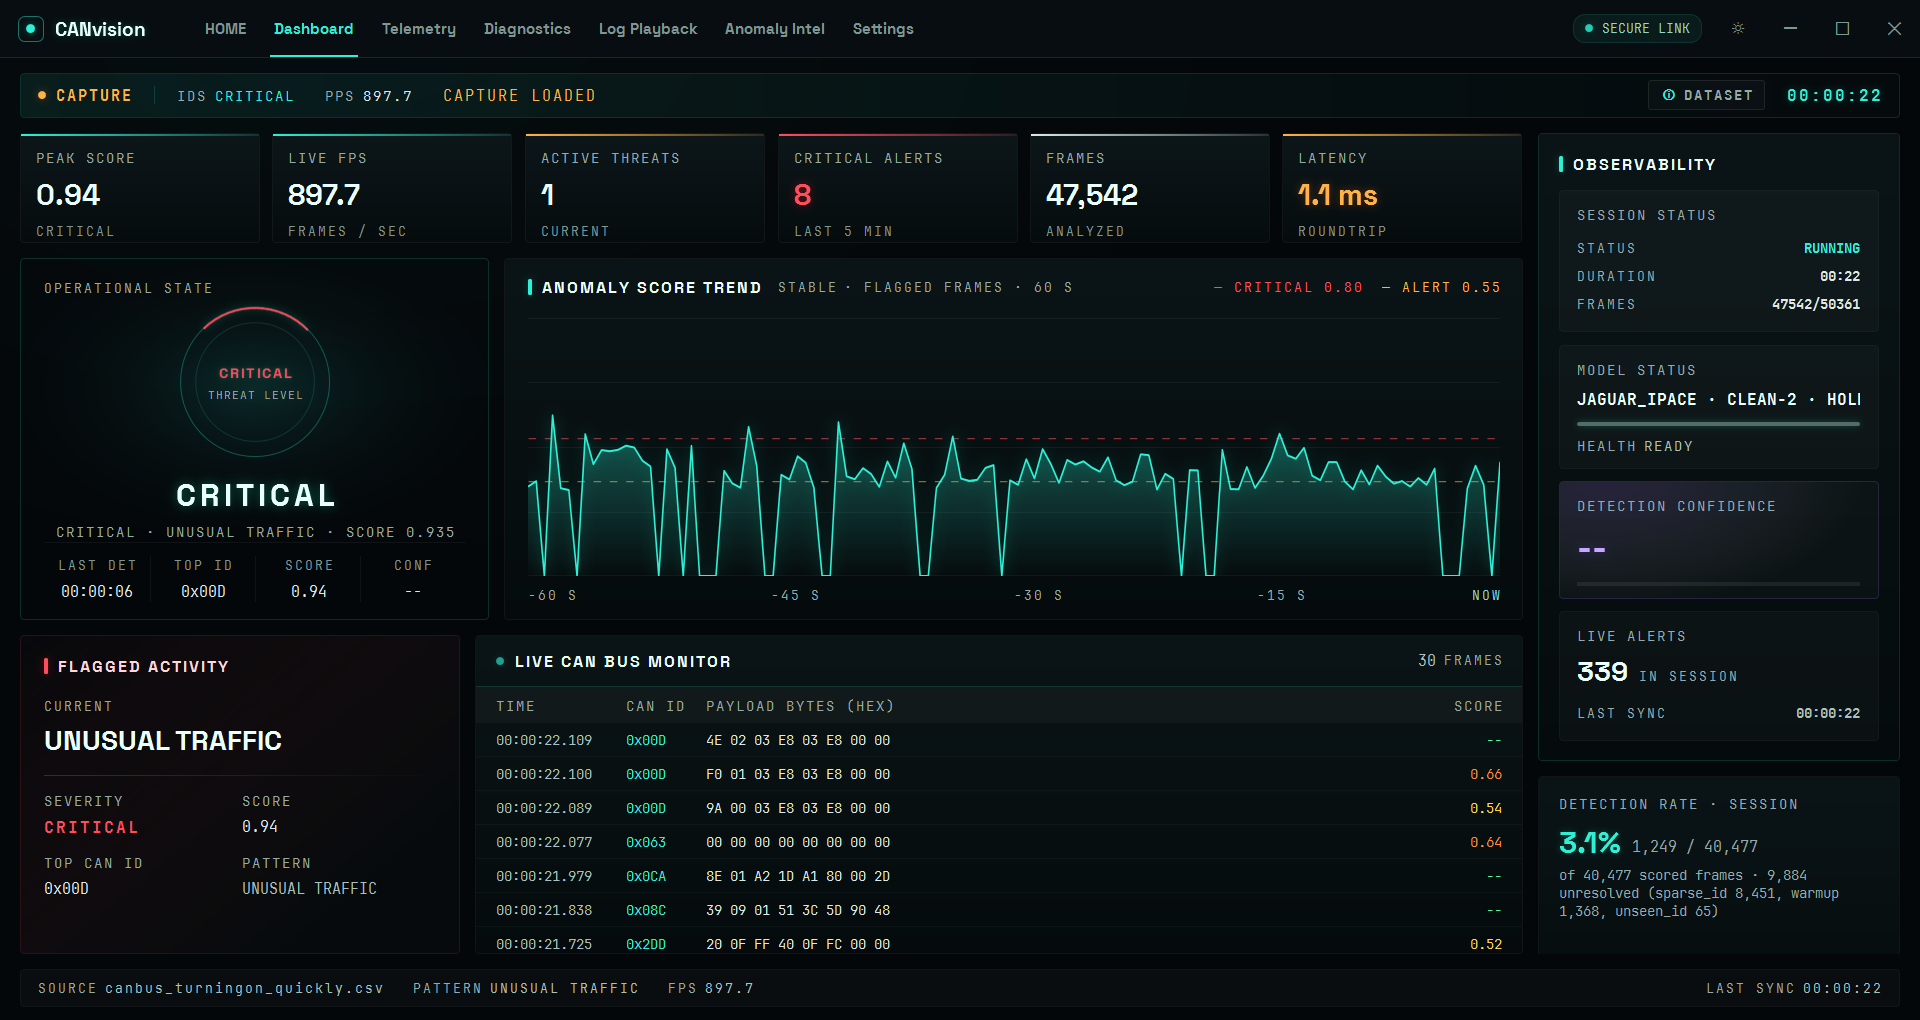
\includegraphics[width=\textwidth]{f02_dashboard.png}
\caption{Dashboard after the analysis of the Jaguar I-PACE holdout recording.}
\label{fig:screen-dashboard-final}
\end{figure}

\begin{itemize}
    \item \textbf{Describe capture:} The Dataset button opens a card that describes the recording in plain words (Figure~\ref{fig:screen-dataset-card}): its number of frames, duration, identifiers and frame rate, and whether the selected model was trained on it, tested on it, or never saw it. Here, it identifies the file as a test recording the model never saw. Without a label file, it states that a flagged frame means ``unusual compared with the training recordings'', not ``confirmed attack''.
\end{itemize}

\begin{figure}[H]
\centering
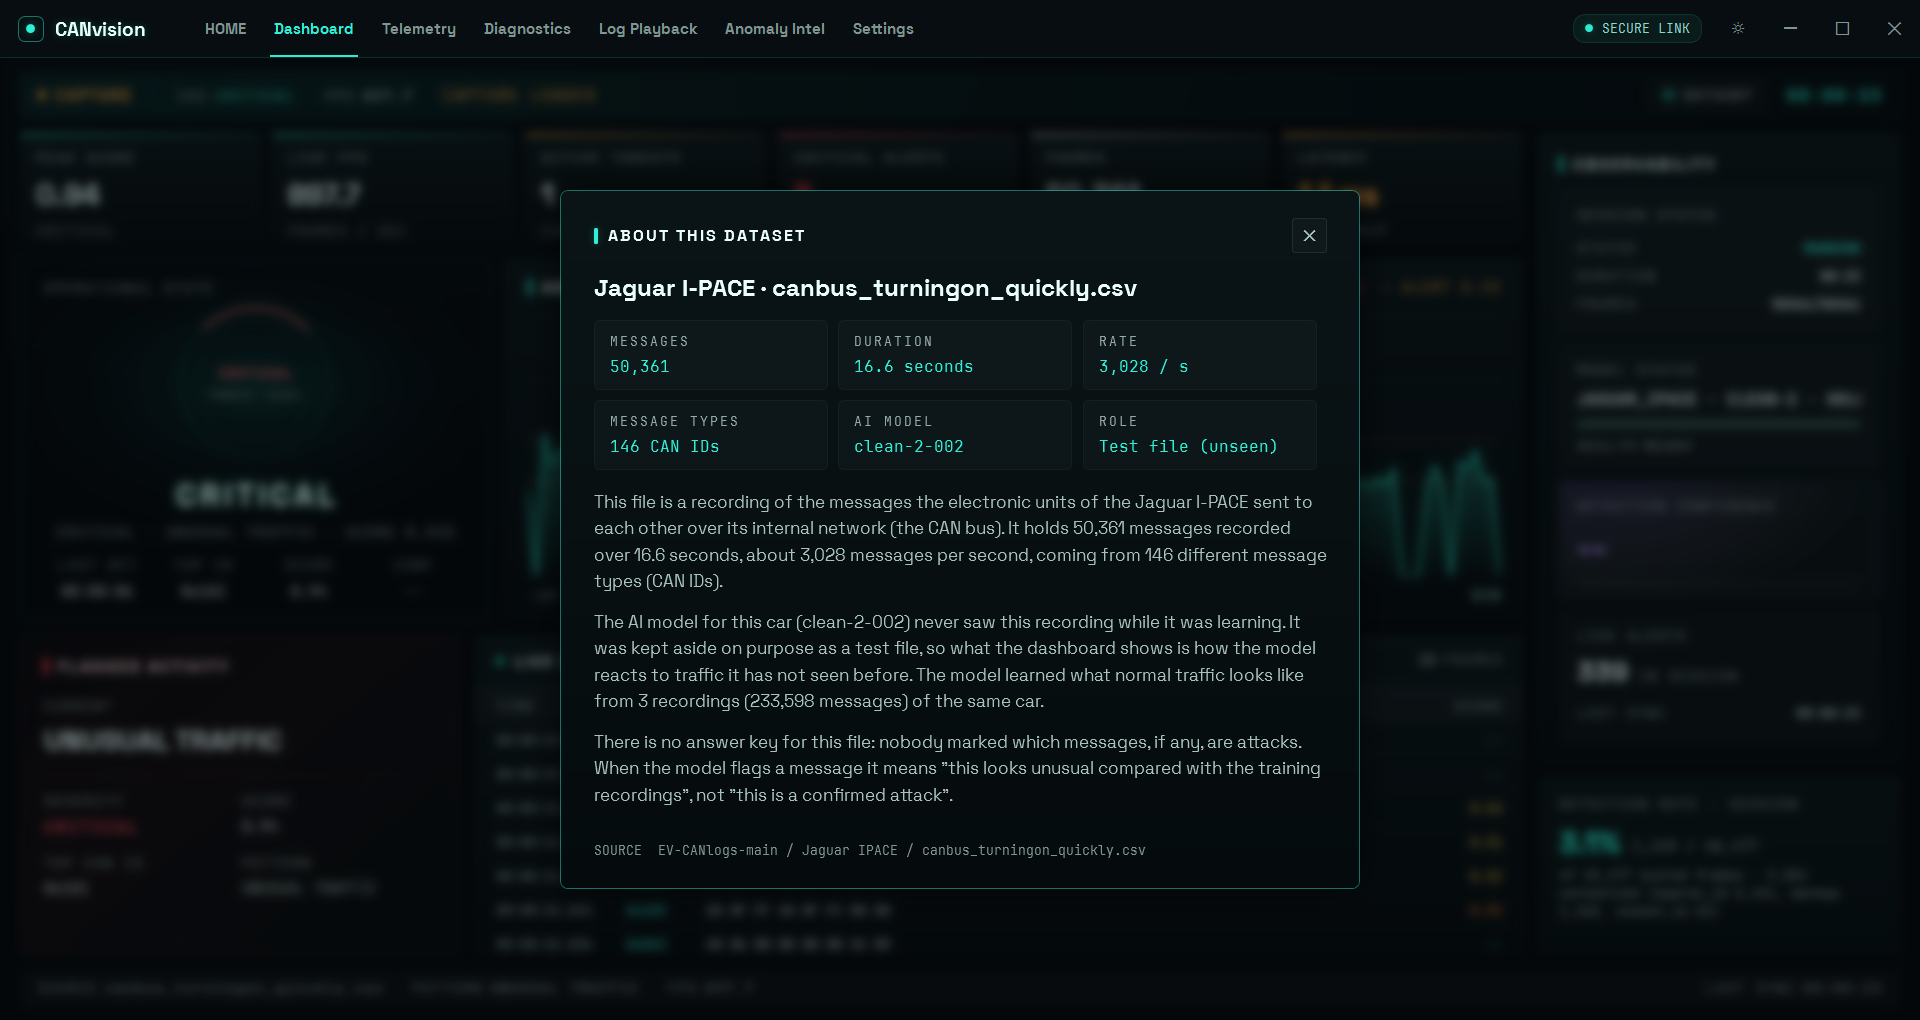
\includegraphics[width=0.9\textwidth]{f02b_dataset_card.png}
\caption{Dataset card of the Jaguar I-PACE holdout recording, open over the Dashboard.}
\label{fig:screen-dataset-card}
\end{figure}

\begin{itemize}
    \item \textbf{Replay log:} The Log Playback screen (Figure~\ref{fig:screen-logplayback}) gives the transport controls and speed, the timeline with the flagged spans, and the detection chart with the threshold of the model.
\end{itemize}

\begin{figure}[H]
\centering
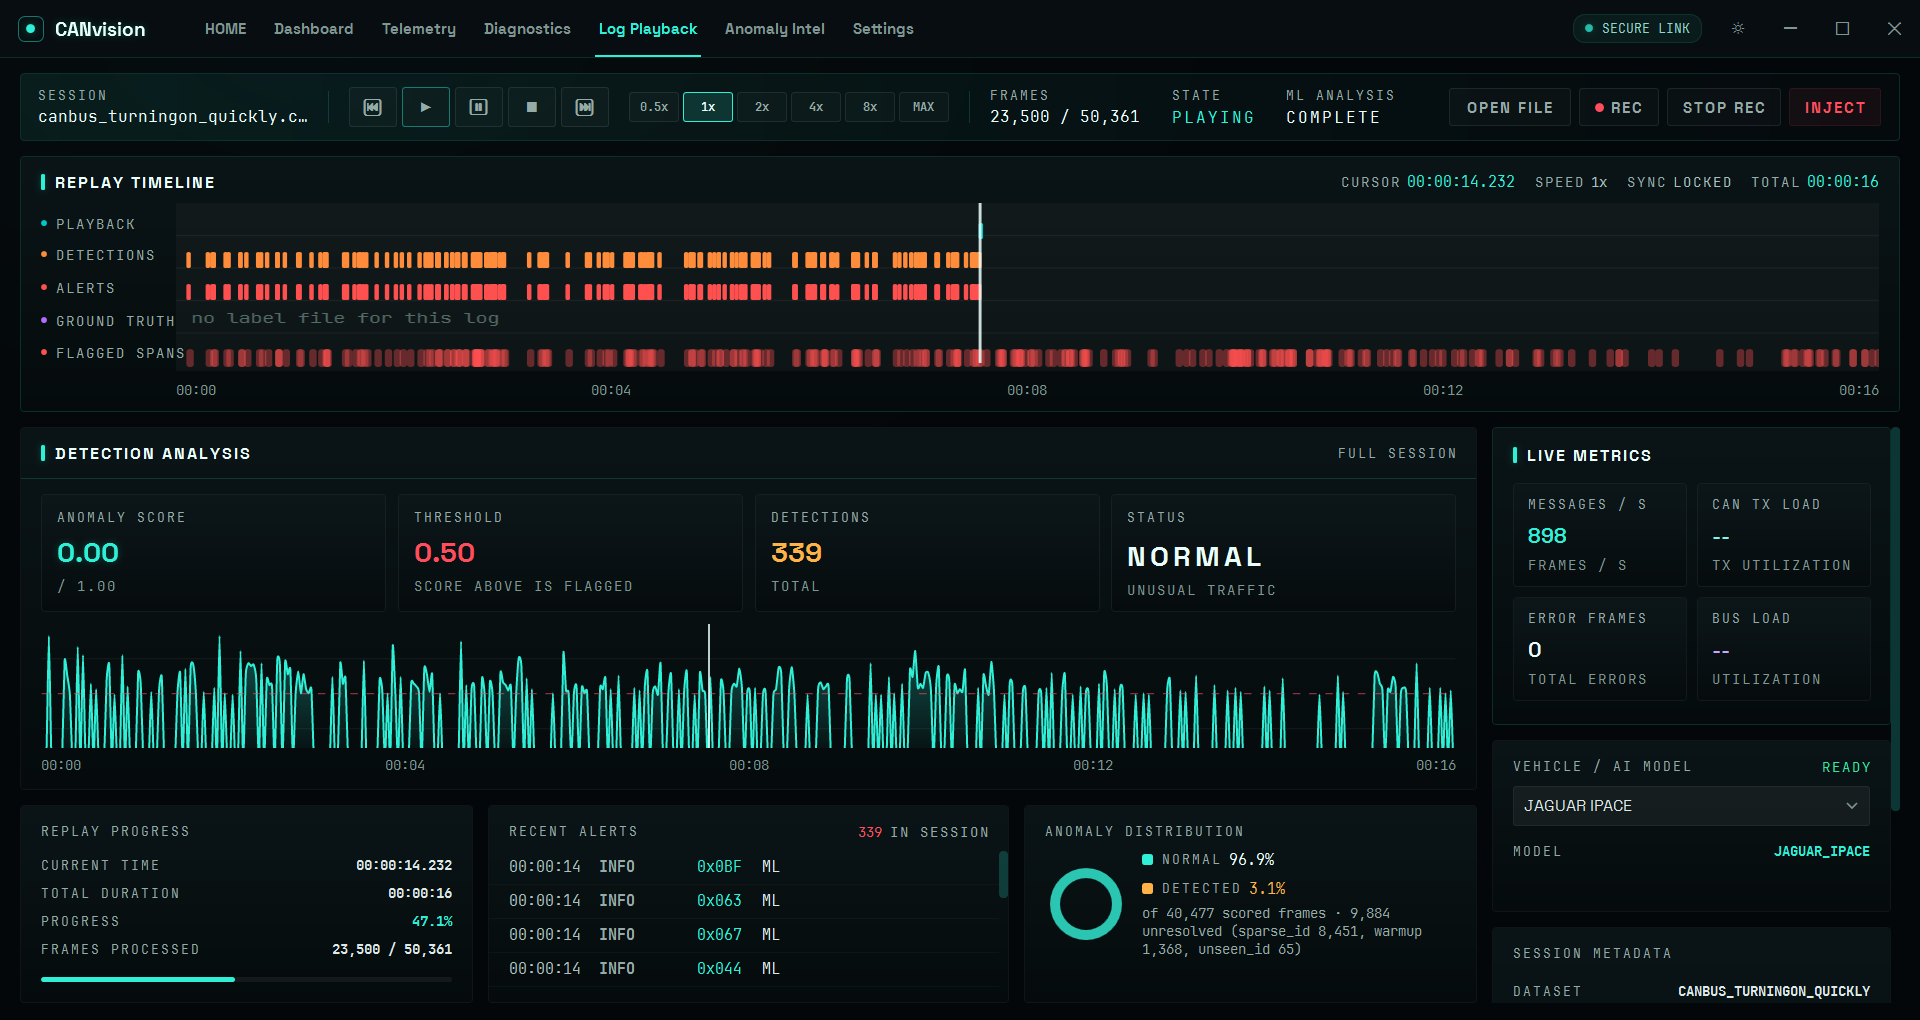
\includegraphics[width=\textwidth]{f07_logplayback.png}
\caption{Log Playback during the replay of the Jaguar I-PACE holdout recording.}
\label{fig:screen-logplayback}
\end{figure}

\Needspace{339pt}% keep the text with its float
\begin{itemize}
    \item \textbf{Review alerts and request an explanation:} Anomaly Intel (Figure~\ref{fig:screen-anomaly-intel}) lists the alerts, shows the signals behind the selected one, and holds the explanation panel. Its alert lists display the offline severities with the labels of Table~\ref{tab:two-paths}.
\end{itemize}

\begin{figure}[H]
\centering
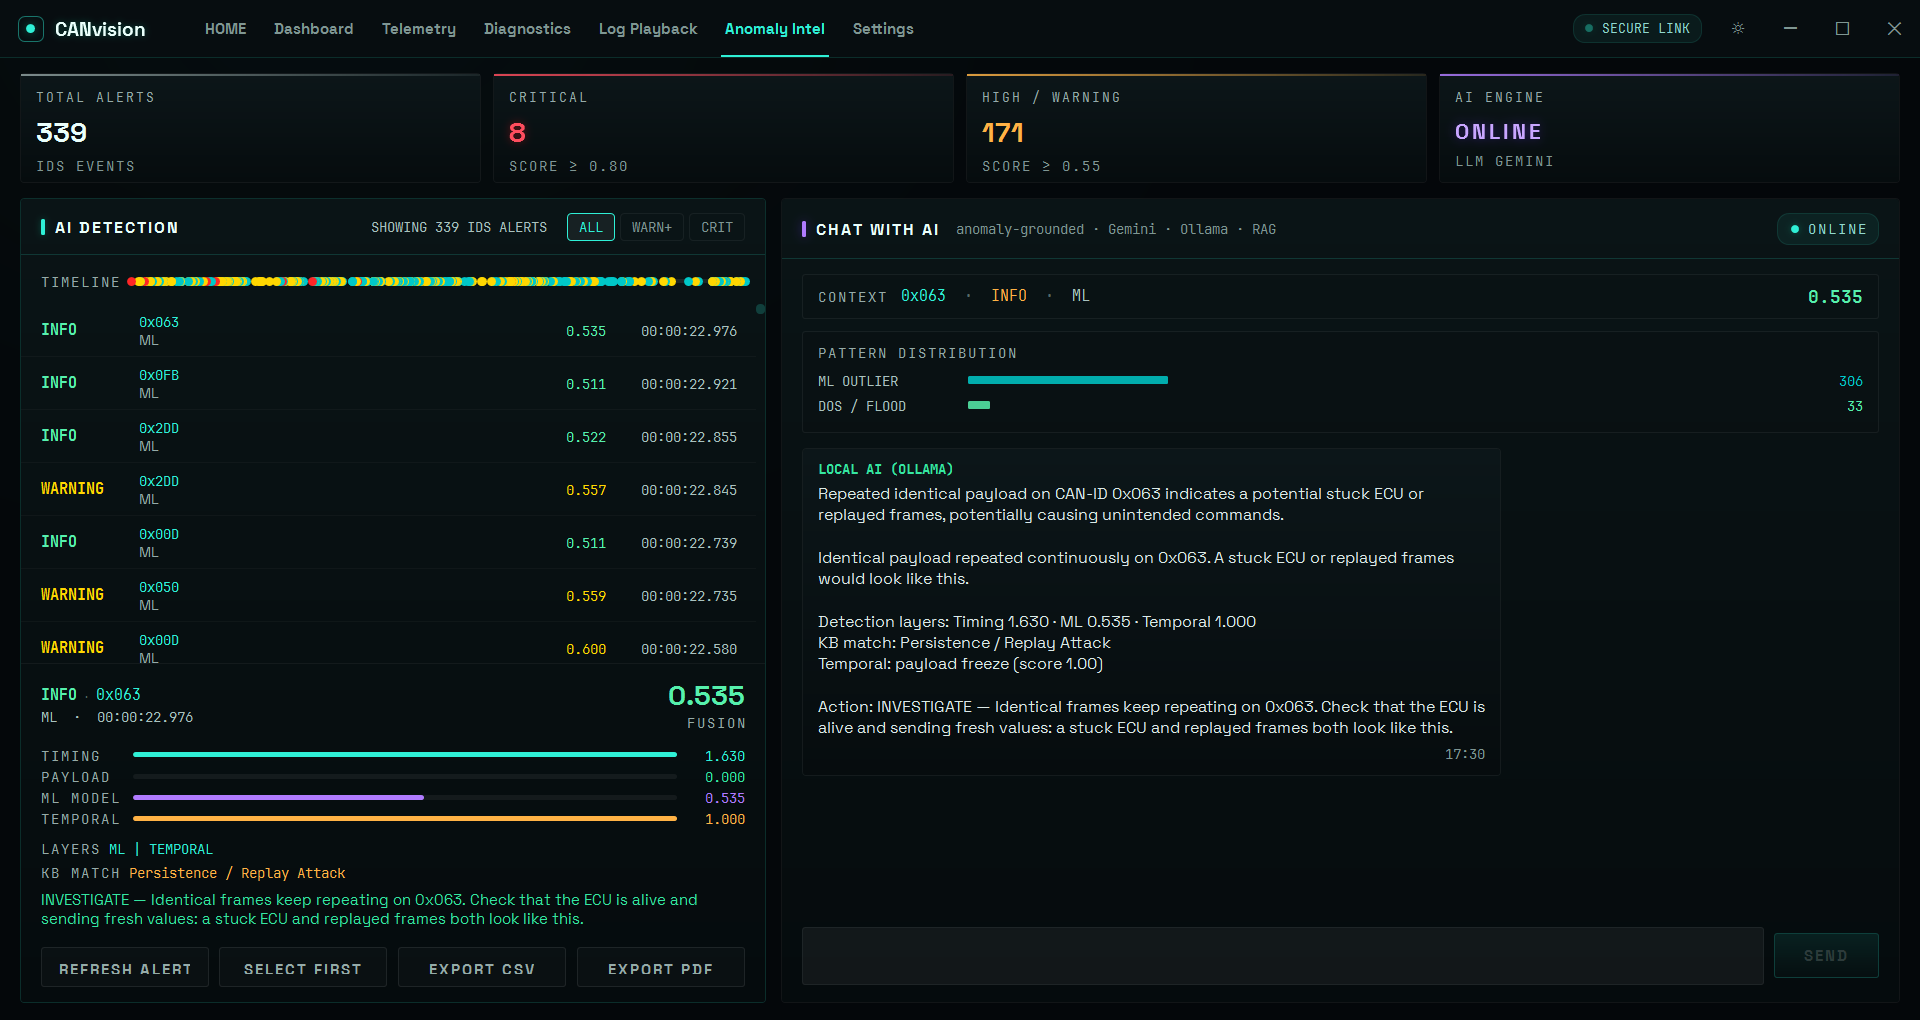
\includegraphics[width=\textwidth]{f08_anomaly_intel.png}
\caption{Anomaly Intel: alert list, signals of the selected alert and explanation panel.}
\label{fig:screen-anomaly-intel}
\end{figure}

\begin{itemize}
    \item \textbf{Export a PDF report:} Anomaly Intel exports the alert list as a PDF report or a \gls{csv} file. The PDF report (Figure~\ref{fig:screen-export-pdf}) gives the session (recording, model and its status, frames analysed, scored, flagged and unresolved), a summary by severity, the identifiers with the most alerts, the alerts in time order, and the explanations requested during the session with the engine that wrote them; for the Jaguar I-PACE analysis it has 13 pages.
\end{itemize}

\begin{figure}[H]
\centering
{\setlength{\fboxsep}{0pt}\setlength{\fboxrule}{0.4pt}\fbox{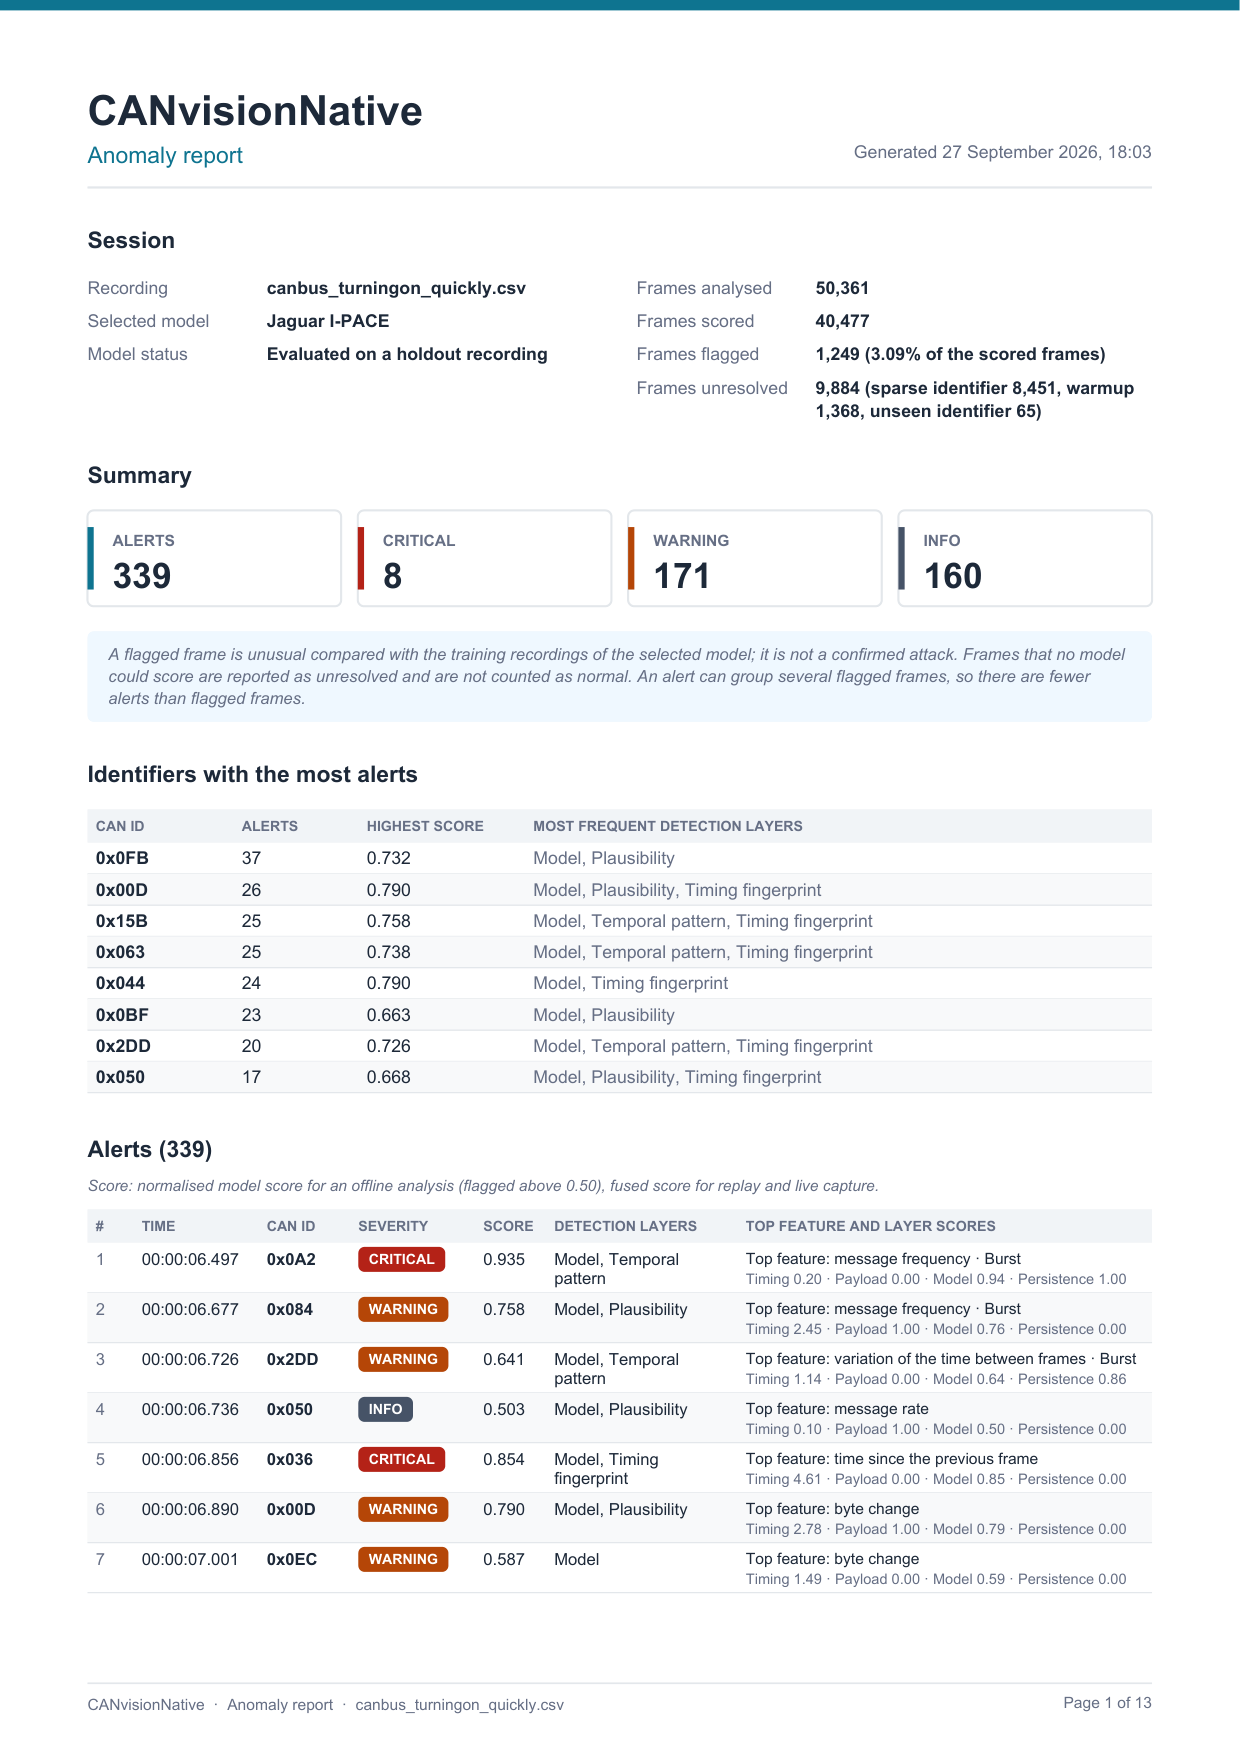
\includegraphics[width=0.62\textwidth]{f10_export_pdf.png}}}
\caption{First page of the PDF report of the Jaguar I-PACE analysis (339 alerts).}
\label{fig:screen-export-pdf}
\end{figure}

\begin{itemize}
    \item \textbf{Export a \gls{csv} file:} The \gls{csv} file (Figure~\ref{fig:screen-export-csv}) has one row per alert, and adds the knowledge base match and the explanation of each alert to the columns of the list.
\end{itemize}

\begin{figure}[H]
\centering
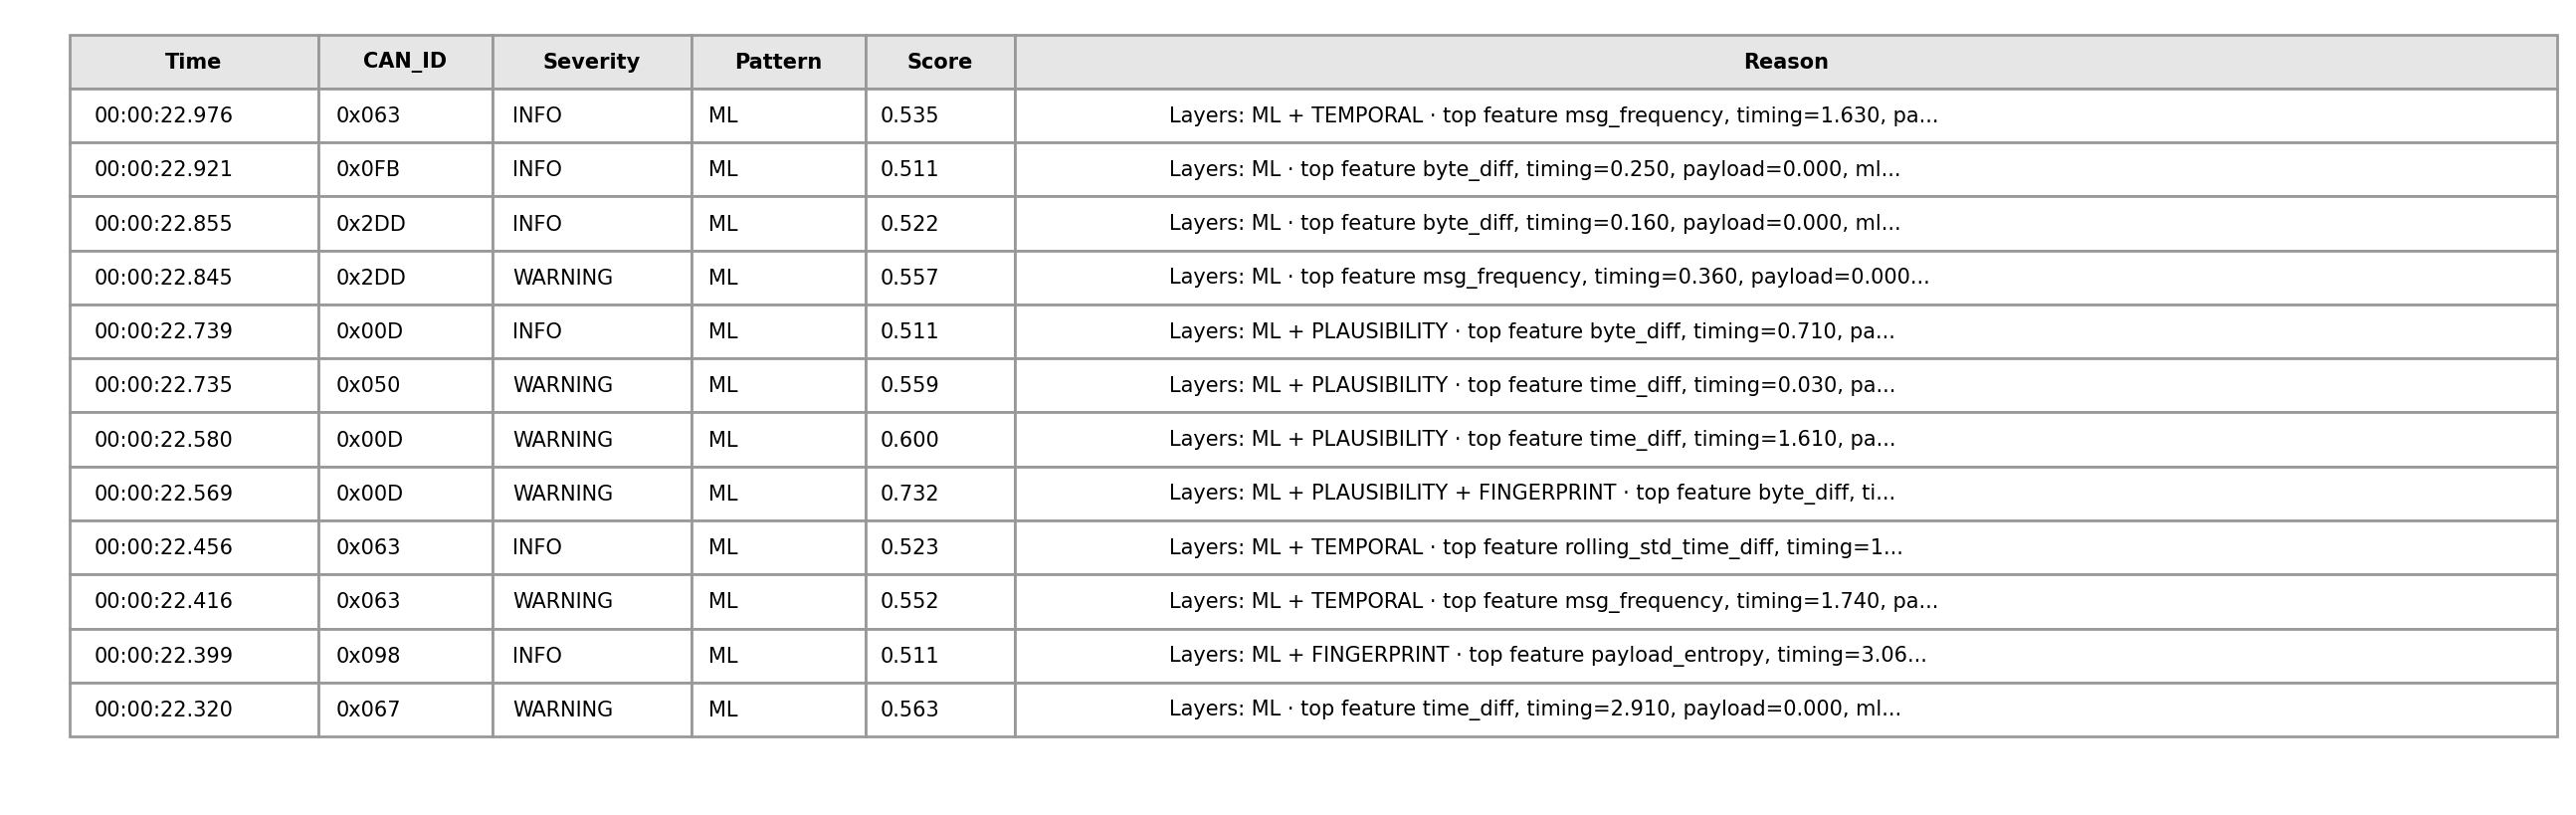
\includegraphics[width=\textwidth]{f09_export_csv.png}
\caption{First rows of the exported \acrshort{csv} file of the same analysis.}
\label{fig:screen-export-csv}
\end{figure}

\begin{itemize}
    \item \textbf{Signals of the capture:} Telemetry (Figure~\ref{fig:screen-telemetry}) shows the signals found in the capture, the live signal monitor and the activity of each identifier. No \gls{dbc} file exists for the Jaguar I-PACE, so the channels are raw payload bytes, labelled as undecoded, as required by FR12. A Diagnostics screen gathers the state of the adapter and the event log of a session.
\end{itemize}

\begin{figure}[H]
\centering
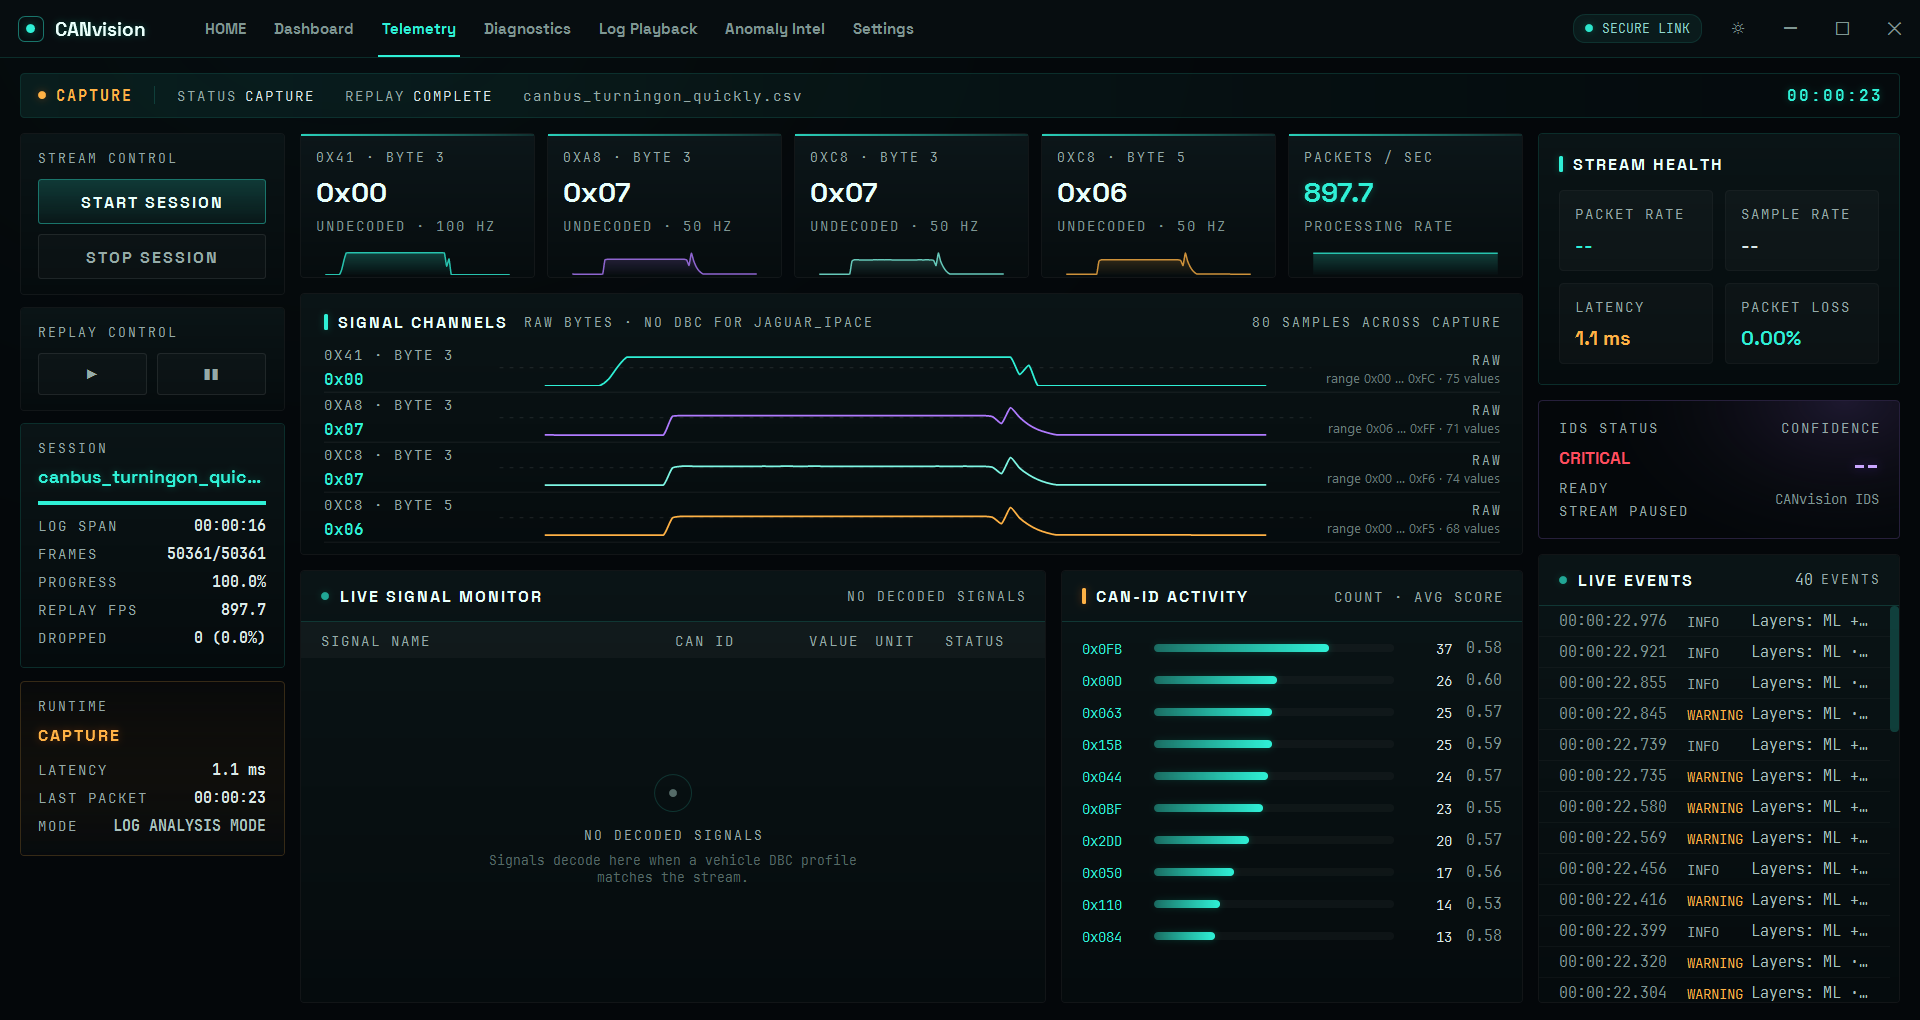
\includegraphics[width=\textwidth]{f03_telemetry.png}
\caption[Telemetry: channels of the Jaguar I-PACE recording.]{Telemetry: channels of the Jaguar I-PACE recording. No \acrshort{dbc} file exists for this vehicle, so the channels are raw payload bytes, marked as undecoded.}
\label{fig:screen-telemetry}
\end{figure}

\begin{itemize}
    \item \textbf{Configure settings:} The Settings screen holds the key of the \gls{llm} provider, the hardware interface (adapter, serial port, bitrate) and an alert threshold, saved locally between sessions. In the current version, this threshold is only stored by the client: it is not sent to the backend, which scores with the values of Table~\ref{tab:two-paths}.
\end{itemize}

\Needspace{690pt}% keep the heading with its float
\section{Test strategy and results}
\label{sec:tests}

\subsection{Test plan}

The same rule applied to every test: a claim had to be backed by reproducible evidence, a defect counted as found only once it could be triggered on demand, and as fixed only once the same test, run again, gave the expected result. Table~\ref{tab:qa-timeline} lists the stages of the validation over the iterations, and Table~\ref{tab:testing-matrix} what each kind of test covered.

\begin{table}[H]
\centering
\footnotesize
\caption{Stages of the validation.}
\label{tab:qa-timeline}
\begin{tabularx}{\textwidth}{|P{4.4cm}|P{2.0cm}|Y|}
\hline
\textbf{Stage} & \textbf{When} & \textbf{Description} \\
\hline
1. Interactive interface audit & Iteration 2 & Exploratory testing of the running application: every screen and every control, actions in the wrong order, destructive actions, resizing and minimising during a replay. \\
\hline
2. Root cause analysis of the alerts & Iteration 2 & Full replay of a one hour Kia EV6 recording, with every alert explained and attributed to a dominant cause. \\
\hline
3. Correction and new validation & Iteration 2 & Each confirmed defect fixed on its own and verified again, then a full run of the corrected pipeline on the same recording. \\
\hline
4. Live capture on the bench rig & Iteration 3 & Frames of the rig read through python-can, then through the hardware layer of the application. \\
\hline
5. Evaluation of the final models & Iteration 4 & Each rebuilt model scored on a complete recording kept out of its training; speed measured; three algorithms compared. \\
\hline
6. End to end test of the release & Transition & The whole application used on a holdout recording, from import to export. \\
\hline
\end{tabularx}
\end{table}

\begin{table}[H]
\centering
\small
\caption{Testing matrix: what was covered, and how.}
\label{tab:testing-matrix}
\begin{tabularx}{\textwidth}{|l|Y|Y|}
\hline
\textbf{Target} & \textbf{Method} & \textbf{Coverage} \\
\hline
Desktop interface & Automation of the running client (clicks, file dialogs, keyboard) and screenshots & Navigation, import, replay controls, actions in the wrong order or repeated \\
\hline
Detection pipeline & Direct calls to the backend \gls{api} and full replays of real recordings & Vehicle selection, scoring, reasons shown to the analyst \\
\hline
Parsers & Small test files per format (\gls{csv}, candump, Vector) and real recordings & Extraction of the frames, byte for byte comparison with a known good output \\
\hline
Final models & Scoring of complete holdout recordings, and checks of each manifest & Flagged rate on new recordings, coverage, consistency of the thresholds \\
\hline
Explanations & Direct \gls{api} calls on two datasets from different vehicles & Correctness per alert, no mixing between sessions or datasets \\
\hline
Live capture & Bench rig, and the virtual bus of python-can in automated tests & Transport of the frames, decoding, alert on an unknown identifier \\
\hline
Export & Manual export and direct inspection of the files & Columns of the \gls{csv} file, rendering and pagination of the PDF \\
\hline
End to end & Full walk through the application (import, analysis, replay, explanation, export) & Integration of every layer, on real recordings \\
\hline
\end{tabularx}
\end{table}

\subsection{Automated tests}

Two automated suites run after every change. The 318 backend tests (pytest) cover the parsers, the manifest checks, the model statuses and refusals, the scoring and the unresolved frames, the threshold calibration, signal discovery, the dataset description, the temporal patterns, the explanation texts and the bench rig profile. The 86 desktop tests (xUnit) cover the import of logs, the \gls{api} contracts, the detection of USB devices, the dataset card, the discovered signals and the PDF report. Both suites pass, and the Release build of the client compiles without warnings.

\subsection{End to end test of the release}
\label{sec:e2e}

Analysing the Jaguar I-PACE holdout file through the application gave the same numbers as the evaluation of Section~\ref{sec:validation-protocol}: 50{,}361 frames, 40{,}477 scored and 1{,}249 flagged (Section~\ref{sec:tour}). This test also revealed display problems, corrected before the screenshots of Section~\ref{sec:tour} were taken. The \gls{csv} exports wrote the scores with the decimal comma of a French Windows installation, which shifted the columns of the file; after the fix, the 339 exported rows all read back with the nine columns of the header. A bus load was shown that was in fact the processing rate of the application divided by twenty. A frequency analysis labelled an identifier sending 0.2 messages per second as a denial of service burst, because its baseline was almost zero. And some explanation texts presented a possible attack as a fact on unlabelled data.

\subsection{Performance}

The offline analysis meets NFR1: the 491{,}969 frames of the Nissan Leaf holdout were analysed in 187 seconds, and the Jaguar I-PACE file in about one minute in the application. The live path processes about 200 to 260 frames per second (Table~\ref{tab:perf-live}), which keeps up with a slow bus such as the one of the Nissan Leaf, but not with buses that carry thousands of frames per second.

\Needspace{385pt}% keep the heading with its float
\section{Requirements traceability}
\label{sec:traceability}

Table~\ref{tab:traceability} links each functional requirement to its implementation and to the evidence that validates it.

\begin{table}[H]
\centering
\footnotesize
\caption{Requirements traceability, from requirement to implementation to validation.}
\label{tab:traceability}
\begin{tabularx}{\textwidth}{|P{1.1cm}|P{6.0cm}|Y|}
\hline
\textbf{Req.} & \textbf{Implemented in} & \textbf{Validated by} \\
\hline
FR1 & Common parser, Section~\ref{sec:impl-parser} & Fix 4, Section~\ref{sec:it2} \\
\hline
FR2 & Vehicle profiles and model selection, Section~\ref{sec:impl-vehicle} & Fix 1, Section~\ref{sec:it2} \\
\hline
FR3 & Replay engine, Section~\ref{sec:impl-replay} & Throughput before and after, Table~\ref{tab:before-after} \\
\hline
FR4 & Detection paths, Section~\ref{sec:design-pipeline}; final models, Section~\ref{sec:impl-feature-eng} & Root cause analysis, Table~\ref{tab:rootcause}; holdout results, Table~\ref{tab:holdout-results} \\
\hline
FR5 & Severity rules, Table~\ref{tab:two-paths} & Severity distribution, Figure~\ref{fig:chart-severity} \\
\hline
FR6 & Explanation engine, Section~\ref{sec:design-ai} & Fix 6, Section~\ref{sec:validation-ai} \\
\hline
FR7 & Exports, Section~\ref{sec:it1} & End to end test, Section~\ref{sec:e2e} \\
\hline
FR8 & Live simulation, Section~\ref{sec:baseline} & Interactive interface audit, Section~\ref{sec:it2} \\
\hline
FR9 & Hardware layer, Section~\ref{sec:impl-hardware} & Bench rig test, Section~\ref{sec:validation-bench}; no vehicle test \\
\hline
FR10 & Session recording, Section~\ref{sec:it1} & Interactive interface audit, Section~\ref{sec:it2} \\
\hline
FR11 & Settings, Section~\ref{sec:tour} & Interactive interface audit, Section~\ref{sec:it2}; the alert threshold is stored but not yet applied \\
\hline
FR12 & Dataset card and signal discovery, Section~\ref{sec:impl-capture} & End to end test, Section~\ref{sec:e2e} \\
\hline
FR13 & Model status and manifest checks, Section~\ref{sec:it4} & Holdout evaluation, Section~\ref{sec:validation-protocol} \\
\hline
\end{tabularx}
\end{table}

Live capture has the weakest evidence: it was tested on a bench rig with synthetic traffic, not on a vehicle.

\section{Deployment and documentation}
\label{sec:deployment}

\subsection{Installation}

The platform is installed on one Windows workstation, as shown in the deployment diagram of Figure~\ref{fig:deployment}. It needs Windows 10 or 11 with .NET Framework 4.8, Python 3.11 or later and Git; a \gls{can} adapter is only needed for live capture. The repository contains a setup guide with the steps below and a troubleshooting section.

\begin{enumerate}
    \item Clone the repository, create a Python virtual environment and install the dependencies of the backend:
\begin{lstlisting}[numbers=none]
python -m venv .venv
.venv\Scripts\activate
pip install -r requirements.txt
\end{lstlisting}
    \item Optionally, give the explanation module a language model: enter a Google Gemini key in the Settings screen of the client, which stores it in the configuration file of the user, or set the variable \code{GOOGLE\_API\_KEY}; or install Ollama and pull a local model, which the backend uses when Gemini is not configured. Without either, the explanations are written by the rule based template.
    \item Start the backend and check that it answers:
\begin{lstlisting}[numbers=none]
python -m uvicorn backend.api.server:app --host 127.0.0.1 --port 8765
curl http://127.0.0.1:8765/health
\end{lstlisting}
    The client also starts the backend by itself when it finds the Python installation.
    \item Start the client, \code{CANvisionNative.exe}. The connection state of the backend is shown in the top right corner of every screen.
\end{enumerate}

\subsection{Model promotion}

New vehicle models are produced and promoted with the commands of the training pipeline (Section~\ref{sec:impl-models}). \code{plan} checks the corpus and prints the split without fitting anything; \code{train} fits a version into the staging folder; \code{validate} checks a staged version; and \code{promote} validates it again and moves it into production, archiving the files it replaces:

\begin{lstlisting}[numbers=none]
python -m backend.ml.training.clean_pipeline plan
python -m backend.ml.training.clean_pipeline train --version <version>
python -m backend.ml.training.clean_pipeline validate --version <version>
python -m backend.ml.training.clean_pipeline promote --version <version>
\end{lstlisting}

A held back vehicle is refused by the promotion step, and the model files in production are versioned with Git LFS.

\subsection{User guide}

Table~\ref{tab:user-guide} gives the main tasks of the analyst and how to perform them.

\begin{table}[H]
\centering
\small
\caption{User guide: main tasks.}
\label{tab:user-guide}
\begin{tabularx}{\textwidth}{|P{3.2cm}|Y|}
\hline
\textbf{Task} & \textbf{How} \\
\hline
Analyse a recording & On Home, import a log file, choose the vehicle model (its status is shown next to it) and run the analysis. The results open on the Dashboard. \\
\hline
Check the dataset & On the Dashboard, open the Dataset card to see the size of the recording and whether the model was trained or tested on it. \\
\hline
Replay a recording & In Log Playback, choose a speed and play; the flagged spans and the alerts appear on the timeline. \\
\hline
Explain an alert & In Anomaly Intel, select an alert; the explanation panel shows the summary, the likely cause, the recommendation and the engine that wrote them. \\
\hline
Export the results & In Anomaly Intel, export the alert list as a PDF report or a \gls{csv} file. \\
\hline
Watch a live bus & Plug in a supported \gls{can} adapter, start a live session on Home, choose the interface, port, bitrate and vehicle model, and connect. \\
\hline
Change the settings & In Settings, set the key of the language model, the hardware interface and the alert threshold, then save. \\
\hline
\end{tabularx}
\end{table}

\section{Stability scope and limitations}
\label{sec:limitations}

Within the scope of this validation, we consider the software stable:

\begin{itemize}
    \item \textbf{All known defects are fixed and verified} with direct evidence.
    \item \textbf{Every model in production was evaluated} on a recording it never saw, and the application shows the status of every model.
    \item \textbf{No silent fallback remains:} Unscored frames are reported with their reason, and a model that may not be used is refused, not replaced.
    \item \textbf{The frame by frame paths share one engine}, and replay and offline analysis share one parser; the offline analysis turns scores into alerts differently (Table~\ref{tab:two-paths}).
    \item \textbf{The pipeline was checked end to end} on real recordings, from import to export.
\end{itemize}

This scope has limits, which we state plainly. It is not a production, safety or security certification, and it does not cover deployment in a vehicle. Live capture was tested only on a bench rig with synthetic traffic, since no compatible vehicle was available, and the run on the physical rig has not been repeated after the last corrections. The final models were evaluated on recordings without attack labels, so we can report flagged rates but no detection rate, precision or recall; we did not evaluate the final models on the labelled attack recordings of public datasets. The live path is too slow for buses above about 260 frames per second. The weights and thresholds of the fused score are fixed configuration values whose effect was not evaluated separately, and the alert threshold shown in the Settings screen is stored but not yet applied to scoring. The coverage of some vehicles is incomplete: on the Jaguar I-PACE, about a fifth of the frames cannot be scored, mostly because they belong to identifiers too rare to have a model. Each vehicle was evaluated on one holdout recording, which says more about that recording than about every driving situation. Finally, the explanations may cite a similar past case, and this history is kept across sessions on purpose, so an analyst who compares two unrelated vehicles may see a past case from the other vehicle.

\section{Conclusion}

The transition phase delivered a release whose screens cover every use case, checked by automated tests and by an end to end test on a recording the models never saw. Every functional requirement is traced to its implementation and its evidence, the platform comes with an installation procedure, a model promotion procedure and a user guide, and its limits are measured and stated.

\chapter*{General Conclusion}
\markboth{\MakeUppercase{General Conclusion}}{\MakeUppercase{General Conclusion}}
\addcontentsline{toc}{chapter}{General Conclusion}

In this report, we presented CANvisionNative, a diagnostic and validation platform for the \gls{can} traffic of Battery Management Systems, built through the four phases of the Unified Process, from its inception to its transition.

We reached the objectives set in Chapter~\ref{chap:framework}, with one exception stated below. The project delivered a Windows desktop client and a Python backend that accept recorded logs, a live simulator and live capture from a \gls{can} adapter. Replay, simulation and live capture share one runtime engine, and the offline analysis of a recording uses the same features and models with its own alert rules. Each vehicle has its own models, one Isolation Forest per \gls{can} identifier, with a threshold calibrated on its training data and a manifest that records how it was built. The four models in production (Jaguar I-PACE, Kia EV6, Nissan Leaf 2019 and the ambient traffic of the ROAD dataset) were trained on 3{,}436{,}061 frames and evaluated on 1{,}130{,}500 frames of recordings they had never seen. An explanation module, separate from detection, describes each alert in plain language. The pipeline was validated on real recordings, and every defect we found was corrected and verified. The exception is live capture: it works on a bench rig of two Arduino boards, but we could not test it on a vehicle, because none was available.

For \gls{can} validation work, CANvisionNative gathers in one tool steps that a BMS engineer usually spreads over several: importing a log in its original format, replaying it, decoding it when a \gls{dbc} file exists, seeing which frames depart from the usual behaviour of their identifier, and reading why. Replay lets the same recording be run again after a change and the results be compared; live monitoring gives a view of the bus when an adapter is connected; the anomaly detection points at the identifiers worth checking first; the explanation turns a score into a text that names the dominant signal and what to check; and the exports keep a trace of the session. The platform reports anomalies, not attacks: it shows which frames it could not judge, the status of each model, and which signals are not decoded.

Besides the client and the backend, the project delivered four vehicle models evaluated on holdout recordings, each with its manifest; a training and promotion pipeline that refuses a model failing its evaluation, as for the MG ZS EV; a bench rig with its firmware and vehicle profile; test suites of 318 backend and 86 desktop tests; and an installation procedure, a model promotion procedure and a user guide. It also produced a method of validation. On the first pipeline, every one of the 15{,}945 alerts of a one hour Kia EV6 recording was attributed to the layer that dominated it before anything was corrected. This led to six silent defects, and correcting them reduced the alerts by a quarter and removed the saturation of the model score, without touching the detection threshold.

Looking back, each principle of the Unified Process left a mark on the project. Because the work was driven by the use cases, each iteration addressed named use cases, and the end to end test of the release walked through all of them on one recording; two of the six defects of the second iteration, the polling timer and the stale explanation, were only found when a use case was followed through the client rather than through the backend alone. Because the work was centred on the architecture, the baseline of the elaboration phase, one runtime engine for replay, simulation and live capture, paid off twice: in the third iteration, live capture only needed its transport to be built and tested, and in the fourth, every vehicle model was replaced without changing the \gls{api} or the screens, apart from the display of the status of each model. Because the work was iterative, the plan could change when the evidence asked for it: the second iteration was meant to validate the first pipeline, and its findings showed that the design of the models itself was fragile, which turned the fourth iteration into a complete rebuild of the models.

The risks of the initial list (Table~\ref{tab:risks}) also proved useful, since several of them materialised and the planned mitigations held. No vehicle was available (R1), and the shared engine and the bench rig allowed live capture to be tested anyway. The wrong model was indeed applied to a vehicle (R3, Fix 1), formats were read differently by different paths (R7, Fix 4), and an explanation could belong to another alert (R8, Fix 6); all three were found and corrected in the second iteration. A model did not generalise to its test recording (R4), and the evaluation step held it back. The live path is too slow for busy buses (R5), and this limit is measured and stated. The first pipeline did raise too many alerts (R6), 16.3\% of the frames, a rate the corrections and the rebuild brought down without touching the threshold. Only the risk on the language model (R2) never materialised, since the chain of providers always produced an explanation.

The main lesson of this work is that the most costly defects were the silent ones: none of them crashed, and each one only appeared when what the system reported was compared with a fact known independently, such as a vehicle being driven or a file being valid. A holdout is only meaningful when the split is made by recording and not by frame, and a flagged rate on unlabelled data is not a detection rate. Working with real logs showed how much the data format matters, from the channel groups of an \gls{mf4} file to the diagnostic polling that shapes the timing of a recording, and the bench rig showed that a single malformed line on a serial link can matter as much as the detection code. Above all, a detection system is only as trustworthy as the evidence behind each of its numbers.

This work also has limits, detailed in Section~\ref{sec:limitations}. Live capture was tested on a bench rig, not on a vehicle. The final models were evaluated on recordings without attack labels, so we report flagged rates, from 0.60\% to 6.09\%, and not a detection rate, a precision or a recall. The live path scores about 200 to 260 frames per second, enough for a slow bus but not for buses that carry thousands of frames per second. Finally, each vehicle was evaluated on one holdout recording, and some vehicles have many identifiers too rare to get a model.

These limits point to the next steps. The first is to validate live capture on a real vehicle, which would close milestone M2. The second is to evaluate the final models on recordings with labelled attacks, such as those of the ROAD dataset, to measure what they detect as well as what they flag. The live path should then be made fast enough for busy buses, for example by scoring several frames at once or by using fewer trees, with each change measured on the holdout recordings. More recordings per vehicle would give a holdout to the vehicles that have none today and a model to more of the rare identifiers.

\cleardoublepage


% ============================================================
% BACK MATTER
% ============================================================
\printbibliography[heading=bibintoc,title={Bibliography}]

% the abstracts, in English and in French, come after the bibliography
\cleardoublepage
\chapter*{Abstract}
\markboth{\MakeUppercase{Abstract}}{\MakeUppercase{Abstract}}
\addcontentsline{toc}{chapter}{Abstract}

Modern vehicles, and electric vehicles in particular, rely on the \gls{can} bus to let their electronic control units exchange data. The \gls{can} protocol was designed for reliability on a closed bus, not for security: it has no authentication and no encryption. In a Battery Management System (BMS), where the \gls{can} traffic carries safety critical values such as cell voltages, state of charge and temperatures, engineers need more than a passive log of the frames.

This report presents \textbf{CANvisionNative}, a diagnostic and validation platform for the \gls{can} traffic of Battery Management Systems, developed at Capgemini Engineering within a work and study program, alongside a full time position as a quality assurance tester of battery management software for BMW Group. The platform combines a Windows desktop client, built with \gls{wpf} and the \gls{mvvm} pattern, with a Python backend that exposes a \gls{rest} \gls{api} built on FastAPI. It imports recorded logs in the common formats, namely \gls{csv}, \gls{mf4}, candump, Vector and PCAN, replays them, and can also receive live traffic from a simulator or from a \gls{can} adapter. Each vehicle has its own machine learning models: one Isolation Forest per \gls{can} identifier, trained on normal traffic, with a threshold calibrated on its training data. The model scores are complemented by timing, payload and persistence checks. An explanation module then describes an alert in plain language, with a language model when one is available and a rule based text otherwise; it does not take part in detection.

The project followed the Unified Process, with four construction iterations. In the second, we explained all 15{,}945 alerts produced by the first pipeline on a one hour Kia EV6 recording and corrected six silent defects, which reduced the alerts by a quarter without changing the detection threshold. In the fourth, we rebuilt the models with a stricter pipeline in which every model records how it was built and enters production only after an evaluation on a complete recording kept out of its training. The four models in production, trained on 3.4 million frames, flag between 0.60\% and 6.09\% of the frames of their test recordings, and a fifth model was held back because its evaluation showed that it could not be trusted. Since the test recordings carry no attack labels, we report these flagged rates and not detection rates. Live capture, delivered in the third iteration, was tested on a bench rig of two Arduino boards but not on a vehicle, and live scoring keeps up only with slow buses, of about 200 frames per second or less.

\vspace{0.5cm}
\noindent\textbf{Keywords:} Controller Area Network, Unified Process, Battery Management System, CAN diagnostics, electric vehicle, anomaly detection, Isolation Forest, holdout evaluation, explainability.

\cleardoublepage

\selectlanguage{french}
\chapter*{Résumé}
\markboth{\MakeUppercase{Résumé}}{\MakeUppercase{Résumé}}
\addcontentsline{toc}{chapter}{Résumé}

Les véhicules modernes, et en particulier les véhicules électriques, reposent sur le bus \gls{can} (Controller Area Network) pour permettre à leurs calculateurs d'échanger des données. Le protocole \gls{can} a été conçu pour la fiabilité sur un bus fermé, et non pour la sécurité : il ne prévoit ni authentification ni chiffrement. Dans un système de gestion de batterie (BMS), où le trafic \gls{can} transporte des valeurs critiques comme la tension des cellules, l'état de charge et la température, les ingénieurs ont besoin de plus qu'un simple enregistrement des trames.

Ce rapport présente \textbf{CANvisionNative}, une plateforme de diagnostic et d'aide à la validation du trafic \gls{can} des systèmes de gestion de batterie, réalisée chez Capgemini Engineering dans le cadre d'un programme d'alternance, en parallèle d'un poste à plein temps de testeur qualité des logiciels de gestion de batterie pour le groupe BMW. La plateforme associe un client de bureau Windows, développé en \gls{wpf} selon le patron \gls{mvvm}, à un backend Python qui expose une \gls{api} \gls{rest} construite avec FastAPI. Elle importe les journaux enregistrés dans les formats courants (\gls{csv}, \gls{mf4}, candump, Vector et PCAN), les rejoue, et peut aussi recevoir un trafic en direct depuis un simulateur ou un adaptateur \gls{can}. Chaque véhicule dispose de ses propres modèles d'apprentissage automatique : une Isolation Forest par identifiant \gls{can}, entraînée sur du trafic normal, avec un seuil calibré sur ses données d'entraînement. Les scores des modèles sont complétés par des contrôles de temporisation, de contenu et de persistance. Un module d'explication décrit ensuite une alerte en langage naturel, avec un modèle de langage lorsqu'il est disponible et un texte à base de règles sinon ; il ne participe pas à la détection.

Le projet a suivi le Processus Unifié, avec quatre itérations de construction. Au cours de la deuxième, nous avons expliqué les 15~945 alertes produites par le premier pipeline sur un enregistrement d'une heure d'une Kia EV6 et corrigé six défauts silencieux, ce qui a réduit les alertes d'un quart sans modifier le seuil de détection. Au cours de la quatrième, nous avons reconstruit les modèles avec une chaîne plus stricte : chaque modèle n'entre en production qu'après une évaluation sur un enregistrement complet exclu de son entraînement. Les quatre modèles en production, entraînés sur 3,4 millions de trames, signalent entre 0,60~\% et 6,09~\% des trames de leurs enregistrements de test, et un cinquième modèle a été écarté car son évaluation a montré qu'il n'était pas fiable. Ces enregistrements ne portant aucune étiquette d'attaque, nous rapportons ces taux de signalement et non des taux de détection. La capture en direct, réalisée lors de la troisième itération, a été testée sur un banc d'essai de deux cartes Arduino, mais pas sur un véhicule, et l'évaluation en direct ne suit que les bus lents, d'environ 200 trames par seconde au plus.

\enlargethispage{3\baselineskip}
\vspace{0.3cm}
\noindent\textbf{Mots-clés :} bus CAN, Processus Unifié, système de gestion de batterie, diagnostic CAN, véhicule électrique, détection d'anomalies, Isolation Forest, évaluation sur données exclues, explicabilité.

\selectlanguage{english}
\cleardoublepage


% ============================================================
% Back cover — official ESPRIT artwork
% (thesis/images/cover_back_bg.jpg, extracted from the filled
% official template). No overlay text: the school name and
% contact details are already part of this artwork.
% ============================================================
\clearpage
\begin{titlepage}
\newgeometry{margin=0cm}
\thispagestyle{empty}

\begin{tikzpicture}[remember picture, overlay]
\node[anchor=north west, inner sep=0pt] at (current page.north west) {
\includegraphics[width=21cm,height=29.7cm]{cover_back_bg.jpg}};
\end{tikzpicture}

\end{titlepage}
\restoregeometry


\end{document}
